% !TeX encoding = windows-1250
% !TeX encoding = windows-1250
% preamble for the RiTeh thesis template

\documentclass[botnum,a4paper,11,oneside,final]{tex_aux/rithesis}
%\usepackage[latin1]{inputenc}
%\usepackage[T1]{fontenc}
%\usepackage[english]{babel}
%%%%%%% adjustment for croatian
\usepackage[croatian]{babel}
\usepackage[cp1250]{inputenc}	% this ensures croatian special letters are correctly printed with Windows
%\usepackage[utf8]{inputenc}		% allegedly this will produc Croatian special letter correctly in Linux
%::::::::::::::::::::::::::::::::::::::::::::::::::::::::::::::::::::::::::::
\usepackage{comment}
\usepackage{enumitem}  % za reguliranje vertikalnoga razmaka izmedju stavki u listi
%\setlist{noitemsep} % or \setlist{nolistsep} to cancel all separations
\setlist[itemize]{itemsep=0pt, topsep=4pt, partopsep=0pt, parsep=1ex}
\setlist[enumerate]{itemsep=0pt, topsep=4pt, partopsep=0pt, parsep=1ex}
\setlist[description]{itemsep=0pt, topsep=4pt, partopsep=0pt, parsep=1ex}
%\setlist[enumerate,1]{leftmargin=1cm}
%\setlist[enumerate,2]{leftmargin=1.5cm}
%::::::::::::::::::::::::::::::::::::::::::::::::::::::::::::::::::::::::::::
\usepackage{datetime}  % automatic months, years, days
\renewcommand{\MONTH}{% renew
  \ifcase\the\month
  \or sije�anj% 1
  \or velja�a% 2
  \or o�ujak% 3
  \or travanj% 4
  \or svibanj% 5
  \or lipanj% 6
  \or srpanj% 7
  \or kolovoz% 8
  \or rujan% 9
  \or listopad% 10
  \or studeni% 11
  \or prosinac% 12
  \fi}
%%::::::::::::::::::::::::::::::::::::::::::::::::::::::::::::::::::::::::::::
%\usepackage{setspace}
%\usepackage{lipsum,lineno}
\usepackage[pangram]{blindtext}
\usepackage{ragged2e}   % poravnavanje teksta
\usepackage{graphicx}	% this enables import of graphics
\usepackage[labelsep=space,format=hang]{caption}  % adjusts caption style
\usepackage{subfig}	% this enables use of subfigures
\usepackage{amsmath}
\usepackage{amssymb}
%\usepackage{fancyhdr}
\usepackage{amsfonts}
%\usepackage{amsthm}
%\usepackage{pdfsync}
% This package is used to tell TeXShop where things are in the PDF file.
% Command-click at any spot in the PDF and it will jump to the corresponding
% location in the source file.
\usepackage{epsfig}		% to use eps figures; maybe not necessary to use here with Mac
\usepackage{epstopdf}	% this automatically converts any eps-figure into a pdf-figure
\usepackage[section]{placeins} % da slika ne upada u sljedeci section

\hyphenation{sko-ko-vi-toj}

\DeclareGraphicsRule{.tif}{png}{.png}{`convert #1 `dirname #1`/`basename #1 .tif`.png}	% this converts any tif-figure into a png-figure (Mac directly supports pdf, jpg, png, and mps formats, but additionally can use tif and eps when they are automatically converted in png, and pdf, respectively, using the above two packages
\DeclareGraphicsExtensions{.pdf,.jpeg,.jpg,.png}  % ekstenzije koje ne treba pisati uz ime slike
\graphicspath{{slike/}}   % mjesto gdje su smjestene slike

%\usepackage{makeidx}	% this enables creation of index
%\usepackage{showidx}
%\makeindex			% this makes index automatically, based on author's entries

%\usepackage{eufrak}
%\usepackage[mathcal]{euscript}
\usepackage{psfrag}
%\usepackage{url} 
\usepackage{pdfcomment}
\usepackage{hyperref}
\hypersetup{
breaklinks,
colorlinks=true,
linkcolor=black,
citecolor=black,
filecolor=black,
urlcolor=black
}

\setcounter{topnumber}{1} \setcounter{bottomnumber}{1}

\newcommand{\navod}[1]{``#1''}

\usepackage{glossaries}
\setacronymstyle{long-short}
\makeglossaries

\usepackage{amsthm}
\theoremstyle{definition}
\newtheorem{definition}{Definicija}[section]

\usepackage{todonotes}
\usepackage{cancel}
\usepackage{ulem}
\usepackage{upgreek}
\usepackage{amssymb}
\usepackage{float}
\usepackage[numbers]{natbib}
\usepackage{notoccite}
\usepackage{makecell}

% pomocu \includeonly moze se kompajlirati samo odredjeno poglavlje, da se skrati vrijeme kompajliranja, dok se ne isprave pogreske u tom poglavlju npr.:

%\includeonly{Poglavlje_1}


\begin{document}

\frontmatter   % - ne dirati

% upisati naziv studija
\degreesubject{Diplomski studij ra�unarstva} % upisati odgovarajuci naziv studija

% upisati vrstu rada
\documenttype{Diplomski rad}  % Zavrsni rad ili Diplomski rad

\title{Metodologija za usporedbu kontekstualiziranih \\ polazi�no-odredi�nih matrica}   % upisati specificni naslov rada

\date{\MONTH~\the\year.}   % ne dirati - mjesec i godina �e se upisati sami

\author{Vjera Turk}  % upisati svoje ime i prezime
\jmbag{0069064924}  % upisati vlastiti JMBAG
\maketitle		% ne dirati

%\makecopyright

% Okruzenje za pisanje posvete. Maknuti komentare ukoliko se �eli napisati posvetu.
%\begin{dedication}
%	Ovo je posveta nekome
%\end{dedication}

\mentor{izv.prof.dr.sc.~Renato Filjar}   % zamijeniti podacima o svojem mentoru
\maketitleabstract

% kreira mjesto za umetnuti stranicu s opisom zadatka - ne dirati
\begin{assignmentpage}
\end{assignmentpage}

% kreira mjesto za umetnuti stranicu s izjavom o samostalnoj izradbi zadatka - ne dirati
\begin{honestystatementpage}
	% !TeX encoding = windows-1250


{ \large 
\vspace{15pt}
% prilagodite ovu izjavu s obzirom na potrebni rod imenice (izradio ili izradila)
%::::::::::::::::::::::::::::::::::::::::::::::::::::::::::::::::::::::::::::::::
Izjavljujem da sam samostalno izradila ovaj rad. \vspace{7cm} \\ 

%::::::::::::::::::::::::::::::::::::::::::::::::::::::::::::::::::::::::::::::::
% ovo ispod nema potrebe dirati!
%:::::::::::::::::::::::::::::::::::::::::::::::::::::::::::::::::::::::::::::::::::
\noindent Rijeka, \MONTH~\thisyear.   
\hspace{5.5cm}
	\verb|_______________|  % pomo�u duzine ove crte regulirati potrebnu sirinu crte za potpis

\begin{flushright}
	\vspace{-15pt}
	Ime Prezime 
	\verb|      |   % pomocu praznih mjesta unutar | | crta, regulirati poravnjanje duzine imena i prezimena s gornjom crtom za potpis
\end{flushright}
%:::::::::::::::::::::::::::::::::::::::::::::::::::::::::::::::::::::::::::::::::::

} % \large
\end{honestystatementpage}

% Okruzenje za pisanje zahvale
\begin{acknowledgments} % staviti znak komentara ukoliko se ne stavlja tekst zahvale
	\vspace{5pt}

\begin{flushleft}
\noindent Zahvaljujem xxxxxx na podr�ci tijekom pisanja ovoga rada i korisnim raspravama i savjetima. Zahvaljujem xxxxx na podr�ku tijekom studiranja.
\end{flushleft}  
\end{acknowledgments}

% kreiranje popisa sadrzaja, slika i tabela - ni�ta ne dirati
\tableofcontents
\listoffigures
\listoftables

\mainmatter		% ne dirati

% Ovdje pomo�u include funkcije ucitavati kreirana poglavlja. Poglavljima dajte logicna imena s obzirom na sadrzaj prikazan u njima (bez razmaka u imenu).
%\chapter{Kako koristiti paket za pisanje zavr�noga rada u \LaTeX-u}
Ovo su uvodne napomene za kori�tenje predlo�ka za pisanje zavr�noga ili diplomskoga rada studenata Tehni�koga fakulteta u Rijeci. Prije kori�tenja paketa, pro�itajte ovaj tekst jer �e vam dati nu�ne uvodne informacije, znatno vam olak�ati i ubrzati ure�ivanje teksta nakon toga, pri �emu �e vas i voditi kroz uporabu ovoga paketa na prakti�an na�in.

Paket je pripremljen tako da student �to prije mo�e pisati vlastiti tekst u ve� pripremljenom predlo�ku koji �e, uz minimalno u�enje sintakse \LaTeX-a, studentu olak�ati urediti svoj rad. U paketu su uklju�ene potrebne upute i sintakti�ke strukture koje bi trebale udovoljiti potrebama ve�ine studenta, a dodatne informacije postoje u dvama priru�nicima koji su uklju�eni u ovom paketu te, naravno, na raznim web stranicama na internetu koje su posve�ene \LaTeX-u (vidi u nastavku).

{\color{red} POZOR: paket treba biti prekopiran negdje na disk ne mijenjaju�i originalnu strukturu mapa (foldera) i ne mijenjaju�i nazive datoteka koje su u mapi \emph{tex\_aux}!}


\section{Opis sadr�aja paketa}
\vspace{-2ex}
Paket se sastoji od:
\begin{itemize}
 \item datoteke \href{run:UPUTE.pdf}{{\color{blue} UPUTE.pdf}} koja sadr�i postupak instalacije potrebnih alata na ra�unalo te kori�tenja paketa. \emph{UPUTE} su bazirane na Windows OS, a korisnici drugih OS-ova si na nazna�enim web lokacijama samo trebaju na�i instalacije za njihov OS.
 %
 \item datoteke \verb|JMBAG_Ime_Prezime.tex| koja je sredi�nja datoteka koja povezuje sve cjeline i kompajliranjem koje se dobije izlazni \verb|JMBAG_Ime_Prezime.pdf| dokument (naravno, tijekom rada, upisat �ete svoj specifi�ni JMBAG i ime i prezime).\\ U ovoj se datoteci inicijalno nalaze i upute za kori�tenje paketa kao i primjeri osnovne uporabe naj�e��ih sintakti�kih struktura u \LaTeX-u koje bi trebale biti dovoljne ve�ini studenata za pisanje rada.
 %
 \item mape \verb|tex_aux| u kojoj su \emph{interne datoteke} koje definiraju stilove, formate i sl.\ koji slu�e u slaganju izlaznoga formata. \textbf{Student/ica s njima ne treba \emph{ni�ta} raditi}, ali one trebaju biti u \verb|tex_aux| mapi pod glavnom mapom zavr�noga rada, kao �to je postavljeno u ovom paketu.
 %
 \item mape \emph{slike} u koju student treba pohraniti sve slike koje �e koristiti u radu. Ime mape se ne smije preimenovati bez boljega poznavanja sintakse \LaTeX-a jer ovaj paket da bi ispravno radio o�ekuje ba� takvo ime mape!
 %
 \item datoteke \verb|sintaksa_cestih_struktura.tex| koja ne sudjeluje izravno u kompajliranju pdf dokumenta, nego slu�i kao repozitorij u kojemu su sadr�ane naj�e��e potrebne sintakti�ke strukture koje su spremne za kopiranje u va� tekst uz minimalnu prilagodbu parametara (npr.\ opis slike, ime datoteke specifi�ne slike koju se ubacuje i proizvoljni ID te slike za kasnije referenciranje).
 %
 \item mape \href{run:prirucnici}{{\color{blue}prirucnici}} u kojoj se nalazi nekoliko najpopularnijih priru�nika za uporabu \LaTeX-a. 
\end{itemize}
%%%%%%%%%%%%%%%%%%%%%%%%%%%%%%%%%%%%%%%%%%%%%%%%%%%%%%%%%%%%%%%

\section{�ime se opremiti za pisanje rada}
Da bi se rad napisao pomo�u \LaTeX-a (a to vrijedi svake lipe!), najprije je na ra�unalo potrebno instalirati:
\begin{enumerate}
	\item obavezno: \LaTeX{} software 
	\item obavezno: editor za ure�ivanje teksta 
	\item neobavezno, ali korisno: softver za opis literature. (Premda dodatni softver nije nu�an jer se popis literature mo�e obraditi i ru�no (no to je manje sofisticirano kod uvr�tavanja referenca), sugeriram instalaciju softvera koji pomo�u intuitivnih su�elja korisniku omogu�ava opis pojedine kori�tene literature (kao mala baza podataka), a potom se pojedina jedinica literature jednostavno ubacuje u tekst, a popis literature se na kraju automatski formira (vi�e o tome pro�itajte u nastavku).
\end{enumerate}

\subsection{Instalacija \LaTeX-a}
\begin{enumerate}
	\item odite na sredi�nji \LaTeX{} portal \cite{latex_project}: \url{http://www.latex-project.org/}
	\item kliknite na poveznicu \href{http://www.latex-project.org/ftp.html}{Getting LaTeX} i potom uo�ite i povucite instalaciju koja odgovara va�em OS-u (npr.\ proTeXt za Windows, MacTeX za Mac, TeX Live za Linux). Pozor: instalacijski paket je velik i mo�e du�e potrajati �ak i na brzoj vezi---dajte si dovoljno vremena za obaviti download.
	\item Instalirajte \LaTeX{} slijede�i upute koje su prilo�ene za odabranu instalaciju (npr.\ proTeXt za Windowse daje kratki pdf s uputama koje vas vode kroz instalaciju korak po korak).
\end{enumerate}

\subsection{Instalacija editora teksta}
Instalirajte editor koji je pogodan za pisanje \LaTeX{} koda. \textbf{Za Windows OS, toplo preporu�am}  \href{http://www.texstudio.org}{{\color{blue} TeXstudio}} \cite{texstudio} jer je bogat opcijama, ugodan za rad i stabilan, a instalacije postoje i za Linux i Mac OS. TeXstudio se zasebno povu�e i instalira na ra�unalo, a neke editore teksta koji ve� do�u u paketu za instalaciju LaTeXa mo�ete ignorirati (npr.\ za Windows je do nedavno bio popularan \emph{TeXnicCenter} i dolazi ve� upakiran u proTeXt-u (a mo�da �ete na�i i \emph{TeXworks}), za Mac je kvalitetan \emph{TeXShop} koji sada tako�er dolazi u paketu s MacTeX-om). 

\label{encoding1} {\color{red} POZOR: Premda �e ovo biti jo� napomenuto na stranici~\pageref{encoding2}, prije samoga po�etka pisanja va�ega rada, �to prije �elim napomenuti sljede�i va�ni detalj: za svaki va� tekst koji pi�ete u editoru teksta, uvjerite se da je kodna stranica postavljena na \navod{windows-1250}, �to je klju�no da bi se u izlaznom pdf-u ispravno ispisivali hrvatski dijakriti�ki znakovi! U TeXstudiu, aktualnu kodnu stranicu se mo�e vidjeti i promijeniti preko maloga izbornika u doljnjem desnom kutu glavnoga prozora, gdje se nalazi opcija ``Encoding''. Ukoliko tu ne pi�e ``windows-1250'', kliknite na izbornik, odaberite opciju ``More Encodings'' pa u potom otvorenom su�elju odaberite kodnu stranicu ``windows-1250 / CP 1250'' i potvrdu sa ``Change To''.}

\subsection{Instalacija programa za opis kori�tene literature}
\emph{Ponavljamo: Kori�tenje BiBTeX programa za opis literature \textbf{nije} neophodno, ali jest korisno. U datoteci po imenu \href{run:Literatura.tex}{{\color{blue}Literatura.tex}}, koja je uklju�ena u ovaj paket, ve� su namje�tene postavke kao da �e se literatura opisati pomo�u BiBTeX programa (npr.\ JabRef-a) i ne treba ni�ta mijenjati, ali ispod toga se mo�e prona�i i upute i za drugi--ru�ni-- na�in (p)opisivanja literature.}

Kao bibtex program za opis literature, preporu�am \href{http://www.jabref.org}{{\color{blue} JabRef}} program \cite{jabref}. To je legalno besplatno dostupni program za Windows OS (ali postoji i za Mac, a i platformski neovisna instalacija) koji nam omogu�ava opisivanje literature na lak na�in pomo�u intuitivnih su�elja, a kao rezultat kreira \emph{BibTeX} datoteku \emph{Literatura.bib} (gdje je (\emph{Literatura} naziv koji korisnik treba dodijeliti pri pohrani JabRef datoteke na disk u slu�aju ovoga predlo�ka, da bi paket funkcionirao) u kojoj je literatura opisana na na�in koji \LaTeX{} razumije. 

Uo�ite da ako ne koristite JabRef, ve� se odlu�ite za ru�ni unos literature, �to se isprva doima jednostavnijim, tada �e vam redoslijed referenca u popisu literature odgovarati to�no redoslijedu koji ste naveli u tom popisu --- dakle morate paziti da redoslijed formirate onim redom kojim pozivate reference u va�em tekstu (�to kod nekog kasnije ubacivanja dodatne reference unutar ve� postoje�ega redoslijeda tra�i brigu da ju se ubaci na odgovaraju�e mjesto u popisu literature), a tako�er trebate paziti i na formatiranje teksta svake reference! 

Za razliku od toga, kori�tenjem JabRef-a, izbjegavate ru�no formiranje popisa literature i ne trebate brinuti o redoslijedu referenca, ve� samo pomo�u JabRefa trebate unijeti sve jedinice literature koju �ete navesti, a \LaTeX{} �e vam automatski formirati listu referenca onim redoslijedom kojim reference bude pozivali u tekstu!

Nakon �to kompajlirate projekt, stvorit �e vam se pomo�na datoteka imena \href{run:JMBAG_Ime_Prezime.bbl}{{\color{blue}JMBAG\_Ime\_Prezime.bbl}} u kojoj �e jedinice literature tijekom kompilacije biti formatirane i odatle se ubacuju u kona�nu verziju teksta. Stoga, \textbf{ukoliko ima ikakvih detalja koje u opisu literature treba prilagoditi, a ne mo�ete automatskim putem}, uvijek vam kao ``zadnja crta obrane'' ostaje otvoriti \verb|bbl| datoteku i tamo ru�no napraviti izmjene. Potom ponovo kompajlirajte projekt i te �e se promjene vidjeti u pdf-u tj.\ ru�no unijete promjene ne�e biti poni�tene sve dok ne obri�ete cijelu datoteku.

Umjesto da rukom pi�ete cijelu bibliografiju, vremenski vam je vjerojatno u�inko\-vitije popis literature generirate uporabom JabRef-a, a potom ako i�ta jo� treba prilagoditi, onda samo to napraviti ru�no u \verb|bbl| datoteci.


\subsubsection{Osnovna uporaba JabRef programa}
Upoznajte se s najva�nijim opcijama u \emph{JabRef}-u:
\begin{itemize}
	\item uo�ite ikonu (pod znakom ``+'' i tekstom \emph{New BibTeX Entry}) za unos nove jedinice literature (npr. knjige, �lanka, web portala i sl.)
	%
	\item kada kliknete za unos nove stavke literature, uo�ite kakvi se sve tipovi literature nude za odabir. Odabirom opcije koja odgovara naslovu koji �elite unijeti, otvorit �e vam se novi prozor s poljima u koja se mo�e unijeti informacije o literaturi. Za odabrani tip literature samo su neka polja obavezna (nalaze se pod karticom (eng.\ \emph{tabom}) \emph{Required fields}), dok se pod drugim karticama mo�e i ne mora unijeti dodatne informacije. U slu�aju na�ih zavr�nih/diplomskih radova, bit �e znatan udjeli literature koja je na internetu pa za formatiranje iste, pro�itajte upute i napomene u nastavku ove sekcije.
	%
	\item kada je vi�e autora, njihova imena se u JabRefu polju za unos autora razdvajaju pisanjem klju�ne rije�i \verb|and| (a ne razmakom, zarezom ili to�ka-zarezom!)
	%
	\item U popisu literature se ne�e uvijek pojam prepisati onako kako ste ga vi zapisali u JabRefu! To je posljedica stilova koji su definirani u \verb|bst| datoteci (ne zamarajte se time sada jer je za naprednu razinu \LaTeX-a). No, ako neki pojam ba� ne ispadne suvislo napisan u popisu literature ili ba� �elite forsirati odre�eni na�in zapisa (�esto slu�aj kada se rije� s velikim slovima ne interpretira onako kako �elite), tada to�no odre�eni zapis mo�ete forsirati na na�in da \verb|{tu rije� ili frazu stavite unutar viti�astih zagrada}|
	%
	\item prije nego pohranite pojedinu stavku pomo�u \emph{Ctrl+S}, \textbf{morate svakoj jedinici literature dodijeliti jedinstveni identifikator}, tzv.\ \emph{Bibtexkey}, �to je jedno od polja koja su obavezna za unos. Mo�ete ru�no upisati neki proizvoljni string, ali pogodnije je generirati ga automatski.\\ Za to u�initi me�u ikonama na vrhu imate ikonu koja izgleda kao (�arobni) �tapi� sa zvjezdicama oko njega, klikom na kojega \emph{JabRef} automatski dodijeli jedinstveni BibTeX \emph{klju�} za tu bibliografsku jedinicu. Pomo�u toga klju�a se poslije bilo kada i bilo gdje u pisanju va�ega rada mo�ete pozvati na tu referencu, a \LaTeX{} �e sve ostalo obaviti za vas tj.\ dodijeliti joj odgovaraju�i broj u tekstu i s tim brojem uvrstiti u popis literature.
	%
	\item korisnik ima mogu�nost i promijeniti uzorak po kojem se kreira struktura automatski generiranoga jedinstvenoga BibTeX klju�a tako da se otvori opcija izbornika \emph{Options $>>$ Preferences $>>$ BibTeX key generator}, gdje je na vrhu prozora prikazan \emph{default} uzorak, npr. \verb|[auth]:[year]| �to zna�i da se klju� kreira na bazi \verb|prezime(autora):godina(rada)|. To se sada mo�e urediti po nekom novom uzorku, no ovako definirani uzorak u biti zadovoljava, a ako igdje ima potrebe za dodatnim razlikovanjem, mo�e se na automatski generiranom klju�u jo� ru�no napraviti korekcija dodavanjem nekog znaka na kraju, kao npr.\ dodavanjem \verb|_a| i sl. (Klikom na karticu \emph{BibTeX source} mo�ete vidjeti kako �e unos va�ih podataka zapravo biti zapisan u va�oj \emph{Literatura.bib} datoteci koja �e se formirati od svih bibliografskih jedinica koje unesete.)
	%
	%
	\item Za \emph{ime} va�e bibliografske datoteke kod pohrane na disk obavezno upi�ite  \emph{Literatura} jer to ime o�ekuje ovaj paket. Pozor: Datoteka \emph{Literatura.bib}, koju ste tako kreirali, mora se nalaziti unutar mape ovoga paketa da bi sve ispravno radilo! U paketu je za primjer ve� kreirana jedna datoteka istoga imena koju za vje�bu student mo�e i otvoriti u \emph{JabRef}-u, ali to su samo pokazne bibliografske jedinice unesene kao primjer, koje student treba u kona�nici zamijeniti svojim bibliografskim jedinicama.
	%
	\item Za ``elektroni�ke'' izvore literature (tj.\ sve �to ste kao informaciju na�li na webu), JabRef nudi tip literature pod nazivom ``Electronic'' (vidi Sl.~\ref{fig:jabref}). U njemu pod karticom (eng.\ tabom) \emph{Optional fields} pod poljem \verb|Title| mo�ete upisati ime web stranice (autor, tvrtka i sl.), pod poljem \verb|url| mo�ete upisati URL adresu te web stranice, a pod poljem \verb|Note| upisati datum kada ste posjetili tu web stranicu (npr.\ \emph{srpanj 2016.} ili \emph{3.~rujna~2016.}). Rezultat toga �e u pdf-u biti da je sve napisano redoslijedom koji je predvi�en u Uputama RiTeha za pisanje diplomskog rada \cite{riteh_upute}, \emph{osim �to u ovom Predlo�ku do sada nisam uspio rije�iti ubacivanje zareza izme�u URL adrese i datuma posjeta toj URL adresi}, koji bi ta dva podatka odvojio, pa je tu potrebna mala ru�na \emph{prilagodba na jedan od ovih dvaju na�ina}:
	\begin{enumerate}[label=\textbf{\roman*)}]
		\item kod unosa datuma u polje \verb|Note| (u su�elju JabRef-a), upi�ite datum na sljede�i na�in: \verb|{, <datum>}|, gdje je \verb|<datum>| va� specifi�ni datum, dok �e \emph{zarez} iza prve zagrade izvr�iti razdvajanje URL adrese i datuma, a \textbf{viti�aste zagrade} osigurati da se to ba� tako to�no prenese u pdf-dokument (uklju�uju�i i da se mjesec napi�e malim po�etnim slovom, �to ina�e ne bi bio slu�aj). (Za neke druge tipove referenca kao npr.\ tip \emph{manual}, zarez vam prije datuma ne�e trebati jer �e naziv literature zavr�iti zarezom.) U Jabrefu vam i ina�e vrijedi da kada �elite forsirati da se pojam ba� to�no u popisu literature zapi�e onako kao ste htjeli, onda se pojam stavi unutar viti�astih zagrada \verb|{kao u ovom primjeru}|.
		\item ako u polju \verb|Note| ne upi�ete datum na prethodno opisani na�in, onda vam u pdf dokumentu ne�e biti upisan zarez izme�u URL adrese i datuma koji ste unijeli, a tako�er �e i mjesec biti napisan velikim po�etnim slovom (�to nije stra�no, ali je manje po�eljno). To mo�ete \emph{ru�no} prilagoditi tako da otvorite \verb|.bbl| datoteku i pomo�u \emph{Find/Replace} operacije sve nazive mjeseca zamijenite na na�in da po�inju malim po�etnim slovom (�to nije te�ko kada vam je ve�ina datuma u popisu literature navedena u istom mjesecu), ali zareze �ete svakako morati ubacivati ru�no u svaku pojedinu stavku literature jer ne�e biti nekog predlo�ka kojim biste to rije�ili automatski pomo�u \emph{Find/Replace} operacije. Na kraju opet kompajlirajte projekt. S obzirom na navedeno, prvi na�in je vremenski �tedljiviji!
	\end{enumerate}
\end{itemize}

%%%%%%%%%%%%%%%%%%%%%%%%%%%%%%%%%%%%%%%%%%%%%%%%%%%


\chapter{Primjeri naj�e��ih sintakti�kih struktura}
Prije stvarnoga po�etka pisanja svoga rada, upoznajte se s osnovnim sintakti�kim strukturama koje �e vam trebati tijekom pisanja rada.

U nastavku su opisane naj�e��e sintakti�ke strukture (dio njih mo�ete na�i i u datoteci \emph{Intro.tex}), a dodatne slo�enije strukture su pohranjene u datoteci \href{run:sintaksa_cestih_struktura.tex}{{\color{blue}sintaksa\_cestih\_struktura.tex}} koja je sastavni dio glave mape ovoga paketa. 

\section{Postavljanje naslova poglavlja i sekcija}
\begin{itemize}
	\item \verb|\chapter{Naslov poglavlja}|: za definiranje naslova poglavlja
	\item \verb|\section{Naslov sekcije}|: za definiranje naslova sekcije unutar poglavlja
	\item \verb|\subsection{Naslov podsekcije}|: za definiranje naslova podsekcije
\end{itemize}


\section{Reference na literaturu} \label{sec:RefLit}
Za referencu na pojedini kori�teni izvor informacije (tj.\ jedinicu literature), koristimo naredbu \\
\verb|\cite{bibtexkey}|, gdje je \emph{bibtexkey} jedinstveni klju� kojim prethodno ozna�imo tu jedinicu literature. \verb|Bibtexkey| mo�emo definirati na jedan od sljede�ih na�ina:
\begin{description}
	\item[I)] ako popis literature definiramo izravno u datoteci \href{run:Literatura.tex}{{\color{blue}Literatura.tex}} (opcija (I) u datoteci), onda ispred svake stavke literature treba definirati i jedinstveni \verb|bibtexkey| pomo�u naredbe \verb|\bibitem{bibtexkey}| (vidi predlo�ak u datoteci)
	\item[II)] ako literaturu opisujemo pomo�u JabRef datoteke \emph{Literatura.bib} (opcija (II) u datoteci), onda se tamo uz svaku stavku definira \verb|bibtexkey| (bude na dnu JabRef obrasca za upis pojedine jedinice literature)
\end{description}
%
Npr.\ ako negdje u tekstu napi�emo \verb|\cite{latex_wiki}|, gdje je \verb|latex_wiki| prethodno definirani \emph{bibtexkey}, tada �e se u tekstu u uglatoj zagradi pokazati broj  te bibliografske jedinice pod kojim se nalazi u popisu literature (Bibliografiji) na kraju rada (u ovom primjeru, to je broj \cite{latex_wiki}).


\section{Referenca na sekciju, sliku, tabelu ili stranicu} \label{sec:RefText}

Za referenciranje na pojedine dijelove teksta unutar rada, koristimo
{\color{red} \verb|\label{ID}|} i {\color{red} \verb|\ref{ID}|} na na�in da se \verb|\label{ID}| postavi uz dio teksta koji �elimo ozna�iti internom oznakom i poslije �emo se u tekstu na to referencirati, a \verb|\ref{ID}| upotrijebimo na mjestu s kojega se referenciramo na dio teksta koji je ranije ozna�en pomo�u \verb|\label{ID}|.

Ako se �elimo referencirati na specifi�nu sliku ili tabelu ili sekciju ili jednad�bu u tekstu, tada unutar bloka toga sadr�aja stavimo oznaku \verb|\label{prefiks:ID_objekta}| gdje je \emph{objekt} slika ili tablica ili sekcija teksta ili jednad�ba, a na �eljenom mjestu u tekstu se na to referiramo pomo�u \verb|\ref{prefiks:ID_objekta}| (u slu�aju referenciranja jednad�be, bolji oblik naredbe je {\color{red} \verb|\eqref{prefiks:ID_objekta}|}).

\verb|ID_objekta| je proizvoljni string (bez razmaka) koji dodijelimo objektu od interesa, a radi preglednijega ure�ivanja teksta, uobi�ajeno je u \LaTeX-u za pojedine tipove oznaka staviti i odgovaraju�i \emph{prefiks}, kao npr.\ \emph{sec} za oznaku sekcije, \emph{fig} za oznaku slike, \emph{tab} za oznaku tabele, \emph{eq} za oznaku jednad�be i sl. (Tako bi za sliku kojoj dodijelimo $ID=prva$ bilo \verb|\label{fig:prva}|, za tablicu \verb|\label{tab:prva}|, za sekciju \verb|\label{sec:prva}|, a za jednad�bu \verb|\label{eq:prva}|.)

Za referencirati se na \emph{stranicu} u tekstu gdje se nalazi ne�to na �to se �elite osvrnuti, koristi naredba {\color{red} \verb|\pageref{prefiks:ID_objekta}|}. Za njenu primjenu se tako�er prethodno treba ozna�iti �eljeni tekst pomo�u naredbe \verb|\label|.

Tako npr.\ mo�emo staviti da je primjer kreiranja tabele \emph{prva} opisan na stranici~\verb|\pageref{tab:prva}|, �to �e za rezultat imati tekst u kojem pi�e ``da je primjer kreiranja tabele \emph{prva} opisan na stranici~\pageref{tab:prva}'' (jer se u tekstu ta tabela nakon kompajliranja npr.\ na�e na stranici 12). Kako god se tekst smanjivao ili pove�avao i navedena tablica mijenjala broj stranice na kojoj se u kona�nici nalazi, mi ne moramo o tome brinuti jer \LaTeX{} brine o tome i na kraju napi�e to�ni broj stranice! (To je jo� jedna o pogodnosti zbog �ega se ljudi i odlu�e, uz ne�to po�etnoga truda, za kori�tenje \LaTeX-a!).



\section{Poveznica na neki dokument ili URL adresu}
Naredbe \verb|\url| i \verb|\href| slu�e za kreiranje poveznice na neku URL adresu ili neki dokument na disku.

{\color{red}\verb|\url{adresa}|} �e otisnuti URL adresu to�no onako kako je \emph{adresa} navedena unutar zagrada.

{\color{red}\verb|\href{akcija:destinacija}{opis}|} �e na papiru/ekranu ispisati tekst \emph{opis} koji je naveden u drugoj zagradi, i izvr�iti \emph{akciju} prema \emph{destinaciji} koja je navedena u prvoj zagradi. 
\emph{Akcija} mo�e npr.\ glasiti \emph{run} ili \emph{mailto}, gdje �e prvi oblik otvoriti mapu ili datoteku staza koje je navedena kao \emph{destinacija}, a drugi oblik pokrenuti pisanje emaila prema email adresi koja je navedena kao \emph{destinacija}.

Ne pretjerujte ipak s uporabom ovih struktura, odnosno uop�e ne morate to koristiti u radu, nego za vanjske reference koristiti samo \verb|\cite{bibtexkey}| naredbu, a za unutra�nje reference (na dijelove teksta) kombinaciju naredbi \verb|\label{ID}| i \verb|\ref{ID}| kako je to opisano u Sekciji~\ref{sec:RefText}. 


\section{Ubacivanje slike}
Sliku mo�emo ubaciti pomo�u sljede�ega bloka naredbi:
\begin{verbatim}
\begin{figure}[!htbp]
	\begin{center}
 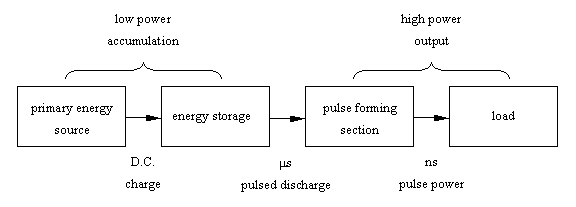
\includegraphics[height=4cm,width=8cm,keepaspectratio=true]{HPMsystem}
 \caption{Primjer ubacivanja slike.}
 \label{fig:prva}
	\end{center}
\end{figure}
\end{verbatim}
Uo�ite uporabu naredbe \verb|\label| unutar bloka. Na nju se potom u tekstu mo�emo referencirati pisanjem npr.\ \verb|Na Slici~\ref{fig:prva}| �ime \LaTeX{} u tekst uvrsti pripadaju�i broj slike, kao npr.\ ``Na Slici~\ref{fig:prva} prikazana je osnovna shema HPM sustava.''
Znak \verb|~| iza rije�i Slici osigurava to�no jedan znak razmaka, �to poma�e ukoliko je rije� Slika na kraju retka, da ne razdvoji rije� Slika i pripadaju�i broj slike.

\begin{figure}[!htbp]
	\begin{center}
 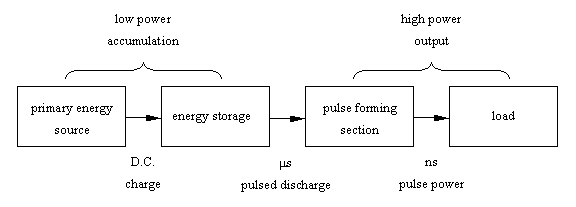
\includegraphics[height=4cm,width=8cm,keepaspectratio=true]{HPMsystem}
 \caption{Primjer ubacivanja slike.}
 \label{fig:prva}
	\end{center}
\end{figure}

Uo�ite i na�in prilago�avanja veli�ine slike. Parametri slike \emph{width} i \emph{height} odre�uju maksimalne dopu�tene dimenzije pri �emu se primarno po�tuje manju navedenu dimenziju, a \emph{keepaspectratio} osigurava zadr�avanje odnosa dimenzija slike, odnosno sprje�ava deformaciju slike, nakon proizvoljno unesenih veli�ina.

Uo�ite da sve oznake tj.\ \emph{labeli} ne smiju imati razmak u imenu. To vrijedi i op�enito, a ne samo za slike.

Tako�er, uo�ite da nije potrebno pisati ekstenziju slike jer to je ure�eno u postavkama glavnoga dokumenta pa time �tedi trud. Ekstenzije koje se mo�e izostaviti su: \emph{jpg}, \emph{jpeg}, \emph{png} i \emph{pdf}.

Shema prikazana na Slici~\ref{fig:prva} �e biti kori�tena i za potrebe idu�ih primjera, a {\color{blue} u mapi na va�em disku ju obri�ite nakon �to po�nete pohranjivati vlastite slike vezane uz va� rad}.


\section{Ubacivanje podslika}
Ponekada se jedna slika sastoji od dvije ili vi�e podslika kojima �elimo opisati neku cjelinu. Slika �e dobiti pripadni broj, a podslike slova (a), (b) itd.
To se mo�e posti�i sljede�om strukturom:
\begin{verbatim}
\begin{figure}[!htpb]
 \begin{center}
  \subfloat[Blok shema HPM sustava.]{\label{fig:HPM}
   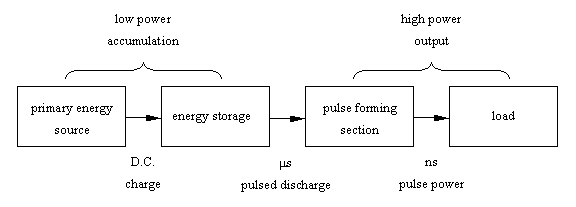
\includegraphics[height=5cm,width=10cm,keepaspectratio=true]{HPMsystem}}\\ 
	    %\hspace{10pt}
   \subfloat[JabRef su�elje za unos ``elektroni�ke'' reference.]
   {\label{fig:jabref}
   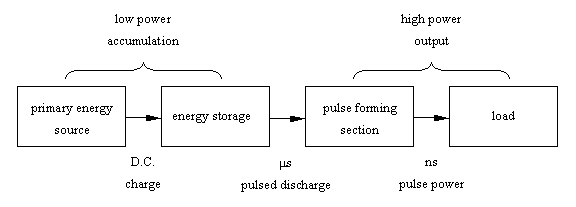
\includegraphics[height=7cm,keepaspectratio=true]{HPMsystem}}
\caption{Primjer ubacivanja vi�e podslika. Ovo je opis cijele slike.}
\label{fig:dvije_podslike}
  \end{center}
\end{figure}
\end{verbatim}
�to �e uvrstiti ono �to se vidi na Slici~\ref{fig:dvije_podslike}, koja se sastoji od dviju podslika.
Podslika~\ref{fig:HPM} pokazuje shemu HPM sustava, a podslika~\ref{fig:jabref} su�elje JabRef programa za unos bibliografskih jedinica.

\begin{figure}[!htpb]
	  \begin{center}
	   \subfloat[Blok shema HPM sustava.]{\label{fig:HPM} 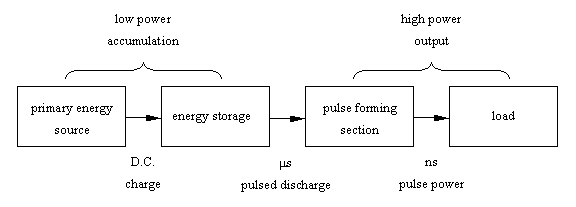
\includegraphics[height=5cm,width=10cm,keepaspectratio=true]{HPMsystem}} \\ %\hspace{10pt}
	   \subfloat[JabRef su�elje za unos ``elektroni�ke'' reference.]{\label{fig:jabref} 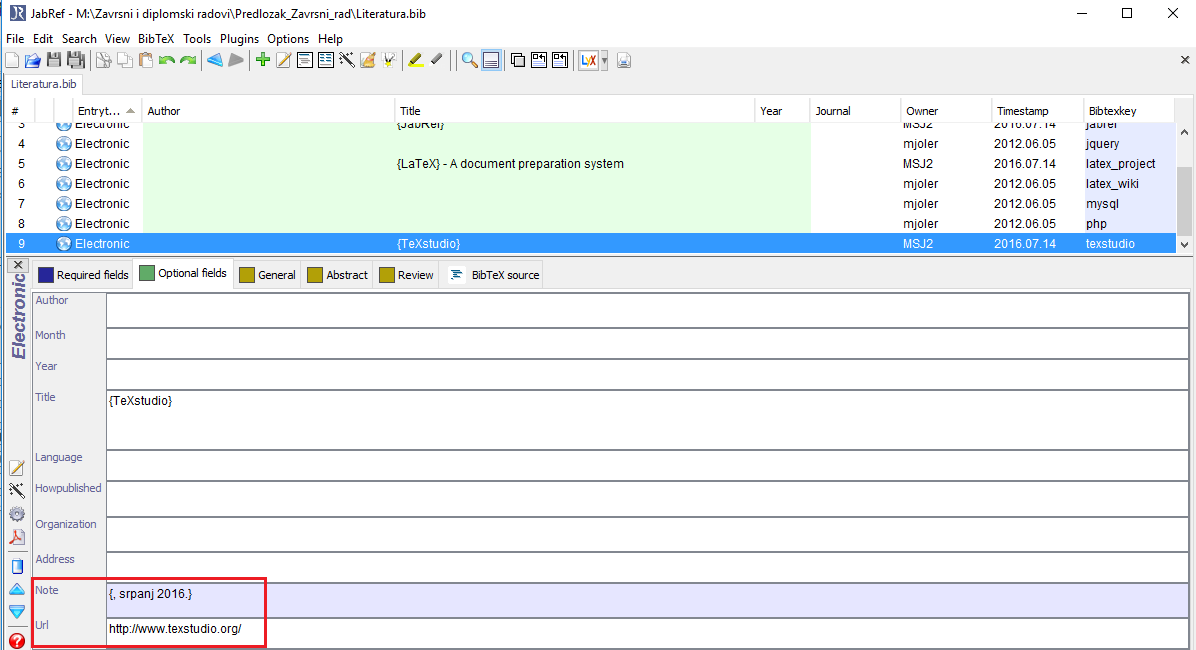
\includegraphics[height=7cm,keepaspectratio=true]{jabref}}
\caption{Primjer ubacivanja vi�e podslika. Ovo je opis cijele slike.}
\label{fig:dvije_podslike}
	  \end{center}
\end{figure}



\section{Ubacivanje tabele} 
Vi�e detalja o kreiranju tabela pro�itajte u literaturi, a sljede�i blok vam omogu�ava kreiranje jednostavne tabele, kao �to je prikazano u Tabeli~\ref{tab:prva}.
\begin{verbatim}
\begin{table}[!htbp]
\renewcommand{\arraystretch}{1.2}
\caption{Ovo je primjer izrade tabele.}
\centering
\begin{tabular}{|c|c|c|}
\hline
variabla & vrijednost 1 & vrijednost 2  \\ [0.5ex]
\hline \hline  
A & 5 & 3 \\ [0.5ex] % razmak do iducega retka
B & 4 & 2 \\ [0.5ex]
\hline
\end{tabular}
\label{tab:prva}
\end{table}
\end{verbatim}

\begin{table}[!htbp]
\renewcommand{\arraystretch}{1.2}
\caption{Ovo je primjer izrade tabele.}
\centering
\begin{tabular}{|c|c|c|}
\hline
variabla & vrijednost 1 & vrijednost 2  \\ [0.5ex]
\hline \hline 
A & 5 & 3 \\ [0.5ex] % razmak do iducega retka
B & 4 & 2 \\ [0.5ex]
\hline
\end{tabular}
\label{tab:prva}
\end{table}
%
Podaci koji su u stupcima se u tabeli razdvajaju znakom \&. Novi redak se na kraju aktualnoga retka formira znakom \verb|\\|. Broj stupaca se definira iza \emph{tabular} time �to se navedu slova koja ozna�avaju poravnavanje teksta u svakom stupcu, a broj slova zna�i broj stupaca koji �e biti kreiran u tabeli. Vertikalni razmak izme�u redaka u tabeli mo�ete za cijelu tabelu prilagoditi uporabom sljede�e sintakse prije strukture za tabelu:\\
\verb| \renewcommand{\arraystretch}{1.2} | gdje broj u zagradi na kraju (ovdje je 1.2) prilagodite sukladno va�oj preferenciji. Mo�e se prilagoditi i razmak za svaki pojedini redak (uo�ite \verb|[0.5ex]| na kraju redaka), ali to je manje od interesa jer tipi�no �elimo da svi retci imaju jednaki razmak jedni od drugih.

Sli�no mo�ete u�initi i za razmak izme�u stupaca tabele navo�enjem sljede�e sintakse prije bloka tabele:\\
\verb| \renewcommand{\tabcolsep}{0.3cm} |.



\section{Uporaba kratica u tekstu. Automatsko generiranje popisa kratica.}  \label{sec:kratice}
Listu kratica definirajte u datoteci \verb|Kratice.tex| (vidjeti predlo�ak unutar datoteke). U redovitom tekstu, kraticu  mo�ete ubaciti kori�tenjem naredbe \verb|\gls{ID_kratice}| gdje je \verb|ID_kraticE| identifikator kratice kako je definiran u datoteci \emph{Kratice.tex}. Pri prvoj uporabi naredbe \verb|\gls|, ispisat �e se najprije puni naziv pojma pa u zagradi kratica, a kod svake sljede�e uporabe, ispisat �e se samo kratica. Na primjer, kada (nakon prethodnog deklariranja u datoteci \verb|Kratice.tex|) upotrijebite \verb|\gls{gsm}| prvi puta, u tekstu �e se ispisati \gls{gsm}, a kada upotrijebite \verb|\gls{gsm}| drugi puta i dalje, u tekstu �e se ispisati samo \gls{gsm} (usporedi s definicijom kratice u datoteci \verb|Kratice.tex|). 
 
{\color{red} Listu kratica generirate sljede�im postupkom:} \label{generiranje_liste_kratica}
\begin{enumerate}
	\item Pokrenite kompilaciju cijeloga teksta jedanputa (to �e generirati neke datoteke koje su potrebne za daljnju obradu, specifi�no one s ekstenzijama .ist i .glo).
	\item Otvorite \emph{Command Prompt} aplikaciju na va�em ra�unalu i postavite se u radnu mapu gdje su vam datoteke za diplomski rad. 
	\item Potom pokrenite \emph{makeindex} rutinu (ona �e tipi�no biti ve� prisutna na va�em ra�unalu) upisuju�i sljede�u sintaksu: \\
	\verb|makeindex   -s myDoc.ist  -o myDoc.gls   myDoc.glo| \\
	gdje naziv datoteke \emph{myDoc} treba zamijeniti nazivom va�e glavne .tex datoteke, (npr. \verb|JMBAG_Ime_Prezime.tex|).
	\item Pokrenite \LaTeX{} jo� jednom ili dva puta, ako treba, dok se u uvodu pdf dokumenta ne pojavi lista kratica (pod naslovom \emph{Pojmovnik}).	
\end{enumerate}

Mo�da isprva zvu�i slo�eno, ali zapravo nije (bar ne uz ovako precizne upute!). Svaki puta kada dodate nove definicije kratica, potrebno je ponoviti ovaj postupak da bi se a�urirale odgovaraju�e datoteke i uredno prikazala potpuna lista u pdf-u (a i izbjegle poruke o pogre�kama tijekom kompajliranja teksta). 

Nije te�ko nakon �to prvi puta pro�ete ovaj postupak i omogu�ava vam u tekstu biti dosljedan u uporabi odre�ene kratice. Da izbjegnete �u�enje, va�no je jo� re�i da �e se ovim postupkom automatski stvoriti tek lista kratica koje ste u tekstu upotrijebili uporabom sintakse \verb|\gls|, a ne na temelju liste definicija koje ste naveli u datoteci \verb|Kratice.tex|. Zato, ako nijednom u tekstu ne upotrijebite sintaksu \verb|\gls|, ne�e biti ispisan ni popis kratica tj.\ \emph{Pojmovnik}. {\color{blue} Kako \LaTeX{} na kraju uvijek nagradi trud koji je ulo�en u savladavanje njegove sintakse, pogodnost ovakvoga automatskoga kreiranja Pojmovnika je i to �to uz svaki kraticu \LaTeX{} automatski ispi�e i brojeve stranica na kojima se doti�na kratica pojavljuje!} U elektroni�kom pdf dokumentu, brojevi stranica su ujedno i hiper-veze na te stranice pa se tako mo�e odmah sko�iti na stranicu gdje je pojedina kratica upotrijebljena.

Ukoliko vam se prethodno opisani postupak �ini preslo�enim, popis kratica mo�ete napraviti i ru�no, isto pomo�u datoteke Kratice.tex, u kojoj tako�er postoji kratki predlo�ak i za takav pristup. Za to je onda u osnovnoj datoteci \verb|JMBAG_Ima_Prezime.tex| potrebno deaktivirati liniju koda koja po�inje sa \verb|\printglossary|, a aktivirati blok koji po�inje sa \verb|\begin{glossary}| i zavr�ava sa \verb|end{glossary}|.



\section{Nagla�avanje teksta}
\subsection{Navodnici}
Za navodnike s lijeve strane fraze (otvaranje navodnika) koristi se 2x jednostruki navodnik koji se na tipkovnici nalazi lijevo od broja 1, a za navodnike s desne strane fraze (zatvaranje navodnika), koristi se 2x jednostruki navodnik koji se na tipkovnici nalazi na tipki \emph{�}, �to proizvede npr.\ ``abc''.

{\color{blue} Alternativno, u ovom paketu je pripremljena i naredba {\color{red} \verb|\navod{abc}|} gdje je \emph{abc} tekst koji se stavlja izme�u navodnika, tj.\ \navod{abc}.}

\subsection{Kosa i podebljana slova}
Nagla�avanje neke rije�i ili fraze pomo�u kosih (italic) slova mo�emo dobiti uporabom naredbe {\color{red} \verb|\emph{abc}|} ili pomo�u  {\color{red}\verb|\textit{abc}|} gdje je \emph{abc} neki tekst koji se �eli naglasiti.

\textbf{Podebljana slova} mo�emo posti�i uporabom naredbe {\color{red} \verb|\textbf{abc}|} gdje je \textit{abc} neki tekst koji �elimo podebljati.

\section{Verbatim: okru�enje za doslovni tekst}
Verbatim okru�enje omogu�ava ispis teksta u izvornom obliku, bez da ga \LaTeX{} tuma�i po svojiim sintakti�kim pravilima. To je pogodno kada se na stranicu  npr.\ �eli kopirati dio programskoga koda iz nekog jezika i kada �elimo zadr�ati sve izvorne znakove u nekoj frazi, bez da \LaTeX{} po�ne javljati pogre�ke kod kompajliranja, �to bi se moglo pojaviti kada se ne bi koristilo \emph{verbatim okru�enje}, po�to bi neke znakove interpretirao kao pogre�ke u sintaksi.

Postoji kra�i i du�i oblik verbatima. Kra�i slu�i za kra�u frazu od jedne ili par rije�i, a du�i za vi�e redaka.

\noindent Kra�i oblik verbatima ima sintaksu: \verb+\verb|neka fraza|+

\noindent Du�i oblik verbatima ima sintaksu:\\
\verb|\begin{verbatim}| \\
\verb|neki tekst| \\
\verb|\end{verbatim}| \\


\section{Kreiranje jedne jednad�be ili serije jednad�ba}

\subsection{Kreiranje jedne jednad�be}
Jednad�ba se napi�e u posebnom matemati�kom modu koji se kreira pomo�u bloka:
\begin{verbatim}
	\begin{equation}
		 A = B + C   \label{eq:prva}
	\end{equation}
\end{verbatim}
�to �e dati sljede�i izgled:
\begin{equation}
	 A = B + C   \label{eq:prva}
\end{equation}
Da bi se na nju referenciralo, na �eljenom mjestu u tekstu upi�emo \verb|\eqref{eq:prva}|, �ime �e se uvrstiti njezin pripadni (automatski generirani) broj, a za potpuniji smisao mo�emo npr.\ napisati \verb| Jednad�ba~\eqref{eq:prva}|, rezultat �ega je da �e u tekstu pisati Jednad�ba~\eqref{eq:prva}. 
Ako ju se ne �eli numerirati, onda se nakon rije�i \emph{begin} stavi zvjezdica, tj.\ \verb|begin*{equation}|.

\subsection{Kreiranje grupe jednad�ba}
Grupa jednad�ba se kreira uporabom \emph{subequations} sintakse. Na primjer, sljede�i blok �e definirati dvije podjednad�be u grupi, gdje �e svaka biti numerirana istim brojem, a razlikovati slovom iza broja.
\begin{verbatim}
	\begin{subequations}
		\begin{align}
		        A &= B + C  	\label{subeq:prva} \\
		        D &= F + G		\label{subeq:druga}
		\end{align}
	\label{subeq:obje}
	\end{subequations}
\end{verbatim}

To �e u izlaznom dokumentu rezultirati sljede�im izgledom:
\begin{subequations}
\begin{align}
        A &= B + C  	\label{subeq:prva} \\
        D &= F + G		\label{subeq:druga}
\end{align}
\label{subeq:obje}
\end{subequations}
U \eqref{subeq:prva} je prikazano dobivanje vrijednosti $A$, a u \eqref{subeq:druga} je prikazano dobivanje vrijednosti $D$. Jednad�ba~\eqref{subeq:obje} je \emph{�uveni studentov zakon}!



\section{Liste}
Liste su �este forme u tekstu kojima se na pregledni na�in nabrajaju neke stavke. Stavke obi�no navodimo ili s to�kama na po�etku, s brojevima ili sa slovima. U \LaTeX-u su upravo ta tri stila unaprijed definirana, a mogu�e su i slo�enije definicije stilova i kombinacije lista.

\subsection{Lista s to�kama}
Lista s to�kama se postigne blokom
\begin{verbatim}
\begin{itemize}
    \item prva nenumerirana stavka
    \item druga nenumerirana stavka
\end{itemize}
\end{verbatim}
�to na ekranu proizvede:
\begin{itemize}
% \setlength\itemsep{1ex}   % za lokalnu prilagodbu
	\item prva nenumerirana stavka
	\item druga nenumerirana stavka
\end{itemize}

\subsection{Lista s brojevima}
Numerirana lista s brojevima se postigne blokom
\begin{verbatim}
\begin{enumerate}[itemsep=1ex, topsep=4pt, partopsep=0pt]
     \item prva numerirana stavka
     \item druga numerirana stavka
\end{enumerate}
\end{verbatim}
U uglatoj zagradi su tri parametra kojima se to�no mo�e kontrolirati vertikalni razmak izme�u stavki u listi (\emph{itemsep}), razmak izme�u prethodnoga teksta i prve stavke u listi (\emph{topsep}) i dodatni prostor izme�u liste i prethodnoga paragrafa kada lista zapo�inje novi paragraf (\emph{partopsep}), ali te parametre \textbf{ne morate navoditi} tj.\ tu uglatu zagradu ne morate pisati. Tada �e se primijeniti vrijednosti parametara koje su definirane za cijeli dokument, a ove parametre se mo�e upotrijebiti tek da u nekom pojedinom slu�aju prilagodite razmake.
Za osjetiti efekte ovih parametara, najbolje se malo sam poigrati razli�itim vrijednostima parametara i vidjeti posljedice toga na listu (pri tome se uz brojeve kao prikladne jedinice za razmak mogu koristiti \emph{pt}, \emph{ex} ili \emph{em}).

\subsection{Proizvoljno ozna�ena lista}
Takva se lista mo�e posti�i u sklopu op�enitije forme koja omogu�uje proizvoljni opis ispred pojedine stavke, pomo�u sljede�ega bloka:
\begin{verbatim}
\begin{description}
     \item[a)] prva opisna stavka
     \item[b)] druga opisna stavka
\end{description}
\end{verbatim}
�to na ekranu proizvede:
\begin{description}%[itemsep=1ex, topsep=4pt, partopsep=0pt] za lokalnu prilagodbu
	\item[a)] prva opisna stavka
	\item[b)] druga opisna stavka \\
\end{description}
%
Kod ove strukture, u uglatu zagradu iza naredbe \verb|\item|, navodi se proizvoljna oznaka kojom se �eli na neki na�in ``numerirati'' listu.
%:::::::::::::::::::::::::::::::::::::::::::::::::::
\chapter{Dodatne informacije}
\section{Primjeri uporabe sintakti�kih struktura}
\begin{enumerate}
	\item Za uvid u kontekstualnu primjenu raznih sintakti�kih struktura, mo�ete otvoriti datoteku \href{run:Intro.tex}{{\color{blue}Intro.tex}}, unutar koje su napisane i ove upute. 
	\item Primjere slo�enijih sintakti�kih struktura, kao �to su ubacivanje slike, tabele ili jednad�be, mo�ete na�i u datoteci \href{run:sintaksa_cestih_struktura.tex}{{\color{blue}sintaksa\_cestih\_struktura.tex}} koja je dio paketa. Odabrane se strukture mo�e kopirati i zalijepiti u va� tekst, uz minimalne prilagodbe kao �to su naziv slike, veli�ina slike, opis i ID slike, a analogno i za tabele i jednad�be.
	\item Kona�no, za vi�e detalja o bilo �emu, potra�ite informacije u dvama priru�nicima koji su prilo�eni u mapi \href{run:prirucnici}{{\color{blue}prirucnici}} ili na webu, gdje se, me�u obiljem drugih informacija, nalaze i korisne wiki stranice \cite{latex_wiki,tex_exchange} o \LaTeX-u pomo�u kojih se obi�no brzo prona�e upute i zadovoljavaju�e rje�enje kakvom sintaksom se mo�e urediti �eljeni dio teksta.
\end{enumerate}

\section{Savjeti za lak�e ure�ivanje teksta}
Vjerujem da vam ovaj dokument mo�e uvelike pomo�i u pripremi teksta va�ega zavr�nog/diplomskog rada i omogu�iti da glavninu vremena tro�ite na sadr�aj rada, a manje na formatiranje rada jer to �e za vas sada obaviti \LaTeX{}! 

No, korektnosti radi, potrebno je napomenuti i sljede�e: \LaTeX{} je vrlo osjetljiv na pogre�ke u sintaksi naredbi (da, ba� kao �to su i programski jezici) pa vas mo�e povremeno ugnjaviti javljanjem pogre�ke koju nikako ne uspijevate uo�iti gdje je. Iskustvo kojim se izbjegava ta nelagoda jest sljede�e:
\begin{itemize}
	\item svako poglavlje napi�ite u novoj datoteci (da biste koli�inu teksta razdvojili na preglednije i manje cjeline) koju imenujte prikladnim imenom (bez razmaka u imenu). Potom te datoteke samo pozivajte iz glavnoga dokumenta \verb|JMBAG_Ime_Prezime.tex| pomo�u naredbe \verb|\include{ime_datoteke}|. Takav je pristup upravo i kori�ten u pripremi ovoga paketa.
	%
	\item {\color{red} budite koncentrirani dok pi�ete \LaTeX{} naredbe, poglavito zagrade, posebne znakove i matemati�ki tekst gdje se zahtijeva uporaba znaka \$!}
	%
	\item kompajlirajte tekst prije nego se skupi puno teksta jer tako �ete imati manje teksta za prekontrolirati u slu�aju pogre�ke. Tako�er vam za provjeru tek manjega dijela dokumenta mo�e pomo�i paket \verb|\usepackage{syntonly}| i naredba \verb|syntaxonly|, a isto tako i naredba \verb|\includeonly{ime_datoteke}| kojom �ete kompajlirati samo tu navedenu datoteku, �ime  ispred ``ne�eljenih'' datoteka ne morate stavljati znak ``komentara'' (\%).
	%
	\item ako niste sigurni ho�e li vam raditi neka naredba nakon pisanja, radije tekst kompajlirajte odmah po pisanju te naredbe---da vidite �to �ete dobiti i rije�ite dvojbu, nego da �ekate da se skupi jo� dubioznih mjesta u tekstu, kada �e nakon kompajliranja biti te�e detektirati koja linija teksta zapravo izaziva probleme (\LaTeX-ov prozor s porukama �esto nije odve� precizan u lociranju i opisu pogre�aka, ovisno o editoru teksta koji koristite).
\end{itemize}


\section{Zavr�ne napomene}
Ovime zaklju�ujemo uvodne upute koje �e najve�em broju studenata biti dovoljne (ili barem dovoljna osnova) za uspje�no pisanje zavr�nog odnosno diplomskog rada.

Prije nego prije�ete na kreiranje vlastitoga sadr�aja u�inite jo� sljede�e akcije kojima �ete deaktivirati dio paketa koji �e biti nepotreban:
\begin{enumerate}
	\item u mapi \href{run:slike}{{\color{blue}slike}}, obri�ite datoteke \verb|HPMsystem.png| i \verb|jabref.png| jer su one slu�ile tek za ilustracije u ovim Uputama.
	%
	\item u glavnoj datoteci  \href{run:JMBAG\_Ime\_Prezime.tex}{{\color{blue}JMBAG\_Ime\_Prezime.tex}} stavite znak komentara ``\%'' ispred linije \verb|\chapter{Kako koristiti paket za pisanje zavr�noga rada u \LaTeX-u}
Ovo su uvodne napomene za kori�tenje predlo�ka za pisanje zavr�noga ili diplomskoga rada studenata Tehni�koga fakulteta u Rijeci. Prije kori�tenja paketa, pro�itajte ovaj tekst jer �e vam dati nu�ne uvodne informacije, znatno vam olak�ati i ubrzati ure�ivanje teksta nakon toga, pri �emu �e vas i voditi kroz uporabu ovoga paketa na prakti�an na�in.

Paket je pripremljen tako da student �to prije mo�e pisati vlastiti tekst u ve� pripremljenom predlo�ku koji �e, uz minimalno u�enje sintakse \LaTeX-a, studentu olak�ati urediti svoj rad. U paketu su uklju�ene potrebne upute i sintakti�ke strukture koje bi trebale udovoljiti potrebama ve�ine studenta, a dodatne informacije postoje u dvama priru�nicima koji su uklju�eni u ovom paketu te, naravno, na raznim web stranicama na internetu koje su posve�ene \LaTeX-u (vidi u nastavku).

{\color{red} POZOR: paket treba biti prekopiran negdje na disk ne mijenjaju�i originalnu strukturu mapa (foldera) i ne mijenjaju�i nazive datoteka koje su u mapi \emph{tex\_aux}!}


\section{Opis sadr�aja paketa}
\vspace{-2ex}
Paket se sastoji od:
\begin{itemize}
 \item datoteke \href{run:UPUTE.pdf}{{\color{blue} UPUTE.pdf}} koja sadr�i postupak instalacije potrebnih alata na ra�unalo te kori�tenja paketa. \emph{UPUTE} su bazirane na Windows OS, a korisnici drugih OS-ova si na nazna�enim web lokacijama samo trebaju na�i instalacije za njihov OS.
 %
 \item datoteke \verb|JMBAG_Ime_Prezime.tex| koja je sredi�nja datoteka koja povezuje sve cjeline i kompajliranjem koje se dobije izlazni \verb|JMBAG_Ime_Prezime.pdf| dokument (naravno, tijekom rada, upisat �ete svoj specifi�ni JMBAG i ime i prezime).\\ U ovoj se datoteci inicijalno nalaze i upute za kori�tenje paketa kao i primjeri osnovne uporabe naj�e��ih sintakti�kih struktura u \LaTeX-u koje bi trebale biti dovoljne ve�ini studenata za pisanje rada.
 %
 \item mape \verb|tex_aux| u kojoj su \emph{interne datoteke} koje definiraju stilove, formate i sl.\ koji slu�e u slaganju izlaznoga formata. \textbf{Student/ica s njima ne treba \emph{ni�ta} raditi}, ali one trebaju biti u \verb|tex_aux| mapi pod glavnom mapom zavr�noga rada, kao �to je postavljeno u ovom paketu.
 %
 \item mape \emph{slike} u koju student treba pohraniti sve slike koje �e koristiti u radu. Ime mape se ne smije preimenovati bez boljega poznavanja sintakse \LaTeX-a jer ovaj paket da bi ispravno radio o�ekuje ba� takvo ime mape!
 %
 \item datoteke \verb|sintaksa_cestih_struktura.tex| koja ne sudjeluje izravno u kompajliranju pdf dokumenta, nego slu�i kao repozitorij u kojemu su sadr�ane naj�e��e potrebne sintakti�ke strukture koje su spremne za kopiranje u va� tekst uz minimalnu prilagodbu parametara (npr.\ opis slike, ime datoteke specifi�ne slike koju se ubacuje i proizvoljni ID te slike za kasnije referenciranje).
 %
 \item mape \href{run:prirucnici}{{\color{blue}prirucnici}} u kojoj se nalazi nekoliko najpopularnijih priru�nika za uporabu \LaTeX-a. 
\end{itemize}
%%%%%%%%%%%%%%%%%%%%%%%%%%%%%%%%%%%%%%%%%%%%%%%%%%%%%%%%%%%%%%%

\section{�ime se opremiti za pisanje rada}
Da bi se rad napisao pomo�u \LaTeX-a (a to vrijedi svake lipe!), najprije je na ra�unalo potrebno instalirati:
\begin{enumerate}
	\item obavezno: \LaTeX{} software 
	\item obavezno: editor za ure�ivanje teksta 
	\item neobavezno, ali korisno: softver za opis literature. (Premda dodatni softver nije nu�an jer se popis literature mo�e obraditi i ru�no (no to je manje sofisticirano kod uvr�tavanja referenca), sugeriram instalaciju softvera koji pomo�u intuitivnih su�elja korisniku omogu�ava opis pojedine kori�tene literature (kao mala baza podataka), a potom se pojedina jedinica literature jednostavno ubacuje u tekst, a popis literature se na kraju automatski formira (vi�e o tome pro�itajte u nastavku).
\end{enumerate}

\subsection{Instalacija \LaTeX-a}
\begin{enumerate}
	\item odite na sredi�nji \LaTeX{} portal \cite{latex_project}: \url{http://www.latex-project.org/}
	\item kliknite na poveznicu \href{http://www.latex-project.org/ftp.html}{Getting LaTeX} i potom uo�ite i povucite instalaciju koja odgovara va�em OS-u (npr.\ proTeXt za Windows, MacTeX za Mac, TeX Live za Linux). Pozor: instalacijski paket je velik i mo�e du�e potrajati �ak i na brzoj vezi---dajte si dovoljno vremena za obaviti download.
	\item Instalirajte \LaTeX{} slijede�i upute koje su prilo�ene za odabranu instalaciju (npr.\ proTeXt za Windowse daje kratki pdf s uputama koje vas vode kroz instalaciju korak po korak).
\end{enumerate}

\subsection{Instalacija editora teksta}
Instalirajte editor koji je pogodan za pisanje \LaTeX{} koda. \textbf{Za Windows OS, toplo preporu�am}  \href{http://www.texstudio.org}{{\color{blue} TeXstudio}} \cite{texstudio} jer je bogat opcijama, ugodan za rad i stabilan, a instalacije postoje i za Linux i Mac OS. TeXstudio se zasebno povu�e i instalira na ra�unalo, a neke editore teksta koji ve� do�u u paketu za instalaciju LaTeXa mo�ete ignorirati (npr.\ za Windows je do nedavno bio popularan \emph{TeXnicCenter} i dolazi ve� upakiran u proTeXt-u (a mo�da �ete na�i i \emph{TeXworks}), za Mac je kvalitetan \emph{TeXShop} koji sada tako�er dolazi u paketu s MacTeX-om). 

\label{encoding1} {\color{red} POZOR: Premda �e ovo biti jo� napomenuto na stranici~\pageref{encoding2}, prije samoga po�etka pisanja va�ega rada, �to prije �elim napomenuti sljede�i va�ni detalj: za svaki va� tekst koji pi�ete u editoru teksta, uvjerite se da je kodna stranica postavljena na \navod{windows-1250}, �to je klju�no da bi se u izlaznom pdf-u ispravno ispisivali hrvatski dijakriti�ki znakovi! U TeXstudiu, aktualnu kodnu stranicu se mo�e vidjeti i promijeniti preko maloga izbornika u doljnjem desnom kutu glavnoga prozora, gdje se nalazi opcija ``Encoding''. Ukoliko tu ne pi�e ``windows-1250'', kliknite na izbornik, odaberite opciju ``More Encodings'' pa u potom otvorenom su�elju odaberite kodnu stranicu ``windows-1250 / CP 1250'' i potvrdu sa ``Change To''.}

\subsection{Instalacija programa za opis kori�tene literature}
\emph{Ponavljamo: Kori�tenje BiBTeX programa za opis literature \textbf{nije} neophodno, ali jest korisno. U datoteci po imenu \href{run:Literatura.tex}{{\color{blue}Literatura.tex}}, koja je uklju�ena u ovaj paket, ve� su namje�tene postavke kao da �e se literatura opisati pomo�u BiBTeX programa (npr.\ JabRef-a) i ne treba ni�ta mijenjati, ali ispod toga se mo�e prona�i i upute i za drugi--ru�ni-- na�in (p)opisivanja literature.}

Kao bibtex program za opis literature, preporu�am \href{http://www.jabref.org}{{\color{blue} JabRef}} program \cite{jabref}. To je legalno besplatno dostupni program za Windows OS (ali postoji i za Mac, a i platformski neovisna instalacija) koji nam omogu�ava opisivanje literature na lak na�in pomo�u intuitivnih su�elja, a kao rezultat kreira \emph{BibTeX} datoteku \emph{Literatura.bib} (gdje je (\emph{Literatura} naziv koji korisnik treba dodijeliti pri pohrani JabRef datoteke na disk u slu�aju ovoga predlo�ka, da bi paket funkcionirao) u kojoj je literatura opisana na na�in koji \LaTeX{} razumije. 

Uo�ite da ako ne koristite JabRef, ve� se odlu�ite za ru�ni unos literature, �to se isprva doima jednostavnijim, tada �e vam redoslijed referenca u popisu literature odgovarati to�no redoslijedu koji ste naveli u tom popisu --- dakle morate paziti da redoslijed formirate onim redom kojim pozivate reference u va�em tekstu (�to kod nekog kasnije ubacivanja dodatne reference unutar ve� postoje�ega redoslijeda tra�i brigu da ju se ubaci na odgovaraju�e mjesto u popisu literature), a tako�er trebate paziti i na formatiranje teksta svake reference! 

Za razliku od toga, kori�tenjem JabRef-a, izbjegavate ru�no formiranje popisa literature i ne trebate brinuti o redoslijedu referenca, ve� samo pomo�u JabRefa trebate unijeti sve jedinice literature koju �ete navesti, a \LaTeX{} �e vam automatski formirati listu referenca onim redoslijedom kojim reference bude pozivali u tekstu!

Nakon �to kompajlirate projekt, stvorit �e vam se pomo�na datoteka imena \href{run:JMBAG_Ime_Prezime.bbl}{{\color{blue}JMBAG\_Ime\_Prezime.bbl}} u kojoj �e jedinice literature tijekom kompilacije biti formatirane i odatle se ubacuju u kona�nu verziju teksta. Stoga, \textbf{ukoliko ima ikakvih detalja koje u opisu literature treba prilagoditi, a ne mo�ete automatskim putem}, uvijek vam kao ``zadnja crta obrane'' ostaje otvoriti \verb|bbl| datoteku i tamo ru�no napraviti izmjene. Potom ponovo kompajlirajte projekt i te �e se promjene vidjeti u pdf-u tj.\ ru�no unijete promjene ne�e biti poni�tene sve dok ne obri�ete cijelu datoteku.

Umjesto da rukom pi�ete cijelu bibliografiju, vremenski vam je vjerojatno u�inko\-vitije popis literature generirate uporabom JabRef-a, a potom ako i�ta jo� treba prilagoditi, onda samo to napraviti ru�no u \verb|bbl| datoteci.


\subsubsection{Osnovna uporaba JabRef programa}
Upoznajte se s najva�nijim opcijama u \emph{JabRef}-u:
\begin{itemize}
	\item uo�ite ikonu (pod znakom ``+'' i tekstom \emph{New BibTeX Entry}) za unos nove jedinice literature (npr. knjige, �lanka, web portala i sl.)
	%
	\item kada kliknete za unos nove stavke literature, uo�ite kakvi se sve tipovi literature nude za odabir. Odabirom opcije koja odgovara naslovu koji �elite unijeti, otvorit �e vam se novi prozor s poljima u koja se mo�e unijeti informacije o literaturi. Za odabrani tip literature samo su neka polja obavezna (nalaze se pod karticom (eng.\ \emph{tabom}) \emph{Required fields}), dok se pod drugim karticama mo�e i ne mora unijeti dodatne informacije. U slu�aju na�ih zavr�nih/diplomskih radova, bit �e znatan udjeli literature koja je na internetu pa za formatiranje iste, pro�itajte upute i napomene u nastavku ove sekcije.
	%
	\item kada je vi�e autora, njihova imena se u JabRefu polju za unos autora razdvajaju pisanjem klju�ne rije�i \verb|and| (a ne razmakom, zarezom ili to�ka-zarezom!)
	%
	\item U popisu literature se ne�e uvijek pojam prepisati onako kako ste ga vi zapisali u JabRefu! To je posljedica stilova koji su definirani u \verb|bst| datoteci (ne zamarajte se time sada jer je za naprednu razinu \LaTeX-a). No, ako neki pojam ba� ne ispadne suvislo napisan u popisu literature ili ba� �elite forsirati odre�eni na�in zapisa (�esto slu�aj kada se rije� s velikim slovima ne interpretira onako kako �elite), tada to�no odre�eni zapis mo�ete forsirati na na�in da \verb|{tu rije� ili frazu stavite unutar viti�astih zagrada}|
	%
	\item prije nego pohranite pojedinu stavku pomo�u \emph{Ctrl+S}, \textbf{morate svakoj jedinici literature dodijeliti jedinstveni identifikator}, tzv.\ \emph{Bibtexkey}, �to je jedno od polja koja su obavezna za unos. Mo�ete ru�no upisati neki proizvoljni string, ali pogodnije je generirati ga automatski.\\ Za to u�initi me�u ikonama na vrhu imate ikonu koja izgleda kao (�arobni) �tapi� sa zvjezdicama oko njega, klikom na kojega \emph{JabRef} automatski dodijeli jedinstveni BibTeX \emph{klju�} za tu bibliografsku jedinicu. Pomo�u toga klju�a se poslije bilo kada i bilo gdje u pisanju va�ega rada mo�ete pozvati na tu referencu, a \LaTeX{} �e sve ostalo obaviti za vas tj.\ dodijeliti joj odgovaraju�i broj u tekstu i s tim brojem uvrstiti u popis literature.
	%
	\item korisnik ima mogu�nost i promijeniti uzorak po kojem se kreira struktura automatski generiranoga jedinstvenoga BibTeX klju�a tako da se otvori opcija izbornika \emph{Options $>>$ Preferences $>>$ BibTeX key generator}, gdje je na vrhu prozora prikazan \emph{default} uzorak, npr. \verb|[auth]:[year]| �to zna�i da se klju� kreira na bazi \verb|prezime(autora):godina(rada)|. To se sada mo�e urediti po nekom novom uzorku, no ovako definirani uzorak u biti zadovoljava, a ako igdje ima potrebe za dodatnim razlikovanjem, mo�e se na automatski generiranom klju�u jo� ru�no napraviti korekcija dodavanjem nekog znaka na kraju, kao npr.\ dodavanjem \verb|_a| i sl. (Klikom na karticu \emph{BibTeX source} mo�ete vidjeti kako �e unos va�ih podataka zapravo biti zapisan u va�oj \emph{Literatura.bib} datoteci koja �e se formirati od svih bibliografskih jedinica koje unesete.)
	%
	%
	\item Za \emph{ime} va�e bibliografske datoteke kod pohrane na disk obavezno upi�ite  \emph{Literatura} jer to ime o�ekuje ovaj paket. Pozor: Datoteka \emph{Literatura.bib}, koju ste tako kreirali, mora se nalaziti unutar mape ovoga paketa da bi sve ispravno radilo! U paketu je za primjer ve� kreirana jedna datoteka istoga imena koju za vje�bu student mo�e i otvoriti u \emph{JabRef}-u, ali to su samo pokazne bibliografske jedinice unesene kao primjer, koje student treba u kona�nici zamijeniti svojim bibliografskim jedinicama.
	%
	\item Za ``elektroni�ke'' izvore literature (tj.\ sve �to ste kao informaciju na�li na webu), JabRef nudi tip literature pod nazivom ``Electronic'' (vidi Sl.~\ref{fig:jabref}). U njemu pod karticom (eng.\ tabom) \emph{Optional fields} pod poljem \verb|Title| mo�ete upisati ime web stranice (autor, tvrtka i sl.), pod poljem \verb|url| mo�ete upisati URL adresu te web stranice, a pod poljem \verb|Note| upisati datum kada ste posjetili tu web stranicu (npr.\ \emph{srpanj 2016.} ili \emph{3.~rujna~2016.}). Rezultat toga �e u pdf-u biti da je sve napisano redoslijedom koji je predvi�en u Uputama RiTeha za pisanje diplomskog rada \cite{riteh_upute}, \emph{osim �to u ovom Predlo�ku do sada nisam uspio rije�iti ubacivanje zareza izme�u URL adrese i datuma posjeta toj URL adresi}, koji bi ta dva podatka odvojio, pa je tu potrebna mala ru�na \emph{prilagodba na jedan od ovih dvaju na�ina}:
	\begin{enumerate}[label=\textbf{\roman*)}]
		\item kod unosa datuma u polje \verb|Note| (u su�elju JabRef-a), upi�ite datum na sljede�i na�in: \verb|{, <datum>}|, gdje je \verb|<datum>| va� specifi�ni datum, dok �e \emph{zarez} iza prve zagrade izvr�iti razdvajanje URL adrese i datuma, a \textbf{viti�aste zagrade} osigurati da se to ba� tako to�no prenese u pdf-dokument (uklju�uju�i i da se mjesec napi�e malim po�etnim slovom, �to ina�e ne bi bio slu�aj). (Za neke druge tipove referenca kao npr.\ tip \emph{manual}, zarez vam prije datuma ne�e trebati jer �e naziv literature zavr�iti zarezom.) U Jabrefu vam i ina�e vrijedi da kada �elite forsirati da se pojam ba� to�no u popisu literature zapi�e onako kao ste htjeli, onda se pojam stavi unutar viti�astih zagrada \verb|{kao u ovom primjeru}|.
		\item ako u polju \verb|Note| ne upi�ete datum na prethodno opisani na�in, onda vam u pdf dokumentu ne�e biti upisan zarez izme�u URL adrese i datuma koji ste unijeli, a tako�er �e i mjesec biti napisan velikim po�etnim slovom (�to nije stra�no, ali je manje po�eljno). To mo�ete \emph{ru�no} prilagoditi tako da otvorite \verb|.bbl| datoteku i pomo�u \emph{Find/Replace} operacije sve nazive mjeseca zamijenite na na�in da po�inju malim po�etnim slovom (�to nije te�ko kada vam je ve�ina datuma u popisu literature navedena u istom mjesecu), ali zareze �ete svakako morati ubacivati ru�no u svaku pojedinu stavku literature jer ne�e biti nekog predlo�ka kojim biste to rije�ili automatski pomo�u \emph{Find/Replace} operacije. Na kraju opet kompajlirajte projekt. S obzirom na navedeno, prvi na�in je vremenski �tedljiviji!
	\end{enumerate}
\end{itemize}

%%%%%%%%%%%%%%%%%%%%%%%%%%%%%%%%%%%%%%%%%%%%%%%%%%%


\chapter{Primjeri naj�e��ih sintakti�kih struktura}
Prije stvarnoga po�etka pisanja svoga rada, upoznajte se s osnovnim sintakti�kim strukturama koje �e vam trebati tijekom pisanja rada.

U nastavku su opisane naj�e��e sintakti�ke strukture (dio njih mo�ete na�i i u datoteci \emph{Intro.tex}), a dodatne slo�enije strukture su pohranjene u datoteci \href{run:sintaksa_cestih_struktura.tex}{{\color{blue}sintaksa\_cestih\_struktura.tex}} koja je sastavni dio glave mape ovoga paketa. 

\section{Postavljanje naslova poglavlja i sekcija}
\begin{itemize}
	\item \verb|\chapter{Naslov poglavlja}|: za definiranje naslova poglavlja
	\item \verb|\section{Naslov sekcije}|: za definiranje naslova sekcije unutar poglavlja
	\item \verb|\subsection{Naslov podsekcije}|: za definiranje naslova podsekcije
\end{itemize}


\section{Reference na literaturu} \label{sec:RefLit}
Za referencu na pojedini kori�teni izvor informacije (tj.\ jedinicu literature), koristimo naredbu \\
\verb|\cite{bibtexkey}|, gdje je \emph{bibtexkey} jedinstveni klju� kojim prethodno ozna�imo tu jedinicu literature. \verb|Bibtexkey| mo�emo definirati na jedan od sljede�ih na�ina:
\begin{description}
	\item[I)] ako popis literature definiramo izravno u datoteci \href{run:Literatura.tex}{{\color{blue}Literatura.tex}} (opcija (I) u datoteci), onda ispred svake stavke literature treba definirati i jedinstveni \verb|bibtexkey| pomo�u naredbe \verb|\bibitem{bibtexkey}| (vidi predlo�ak u datoteci)
	\item[II)] ako literaturu opisujemo pomo�u JabRef datoteke \emph{Literatura.bib} (opcija (II) u datoteci), onda se tamo uz svaku stavku definira \verb|bibtexkey| (bude na dnu JabRef obrasca za upis pojedine jedinice literature)
\end{description}
%
Npr.\ ako negdje u tekstu napi�emo \verb|\cite{latex_wiki}|, gdje je \verb|latex_wiki| prethodno definirani \emph{bibtexkey}, tada �e se u tekstu u uglatoj zagradi pokazati broj  te bibliografske jedinice pod kojim se nalazi u popisu literature (Bibliografiji) na kraju rada (u ovom primjeru, to je broj \cite{latex_wiki}).


\section{Referenca na sekciju, sliku, tabelu ili stranicu} \label{sec:RefText}

Za referenciranje na pojedine dijelove teksta unutar rada, koristimo
{\color{red} \verb|\label{ID}|} i {\color{red} \verb|\ref{ID}|} na na�in da se \verb|\label{ID}| postavi uz dio teksta koji �elimo ozna�iti internom oznakom i poslije �emo se u tekstu na to referencirati, a \verb|\ref{ID}| upotrijebimo na mjestu s kojega se referenciramo na dio teksta koji je ranije ozna�en pomo�u \verb|\label{ID}|.

Ako se �elimo referencirati na specifi�nu sliku ili tabelu ili sekciju ili jednad�bu u tekstu, tada unutar bloka toga sadr�aja stavimo oznaku \verb|\label{prefiks:ID_objekta}| gdje je \emph{objekt} slika ili tablica ili sekcija teksta ili jednad�ba, a na �eljenom mjestu u tekstu se na to referiramo pomo�u \verb|\ref{prefiks:ID_objekta}| (u slu�aju referenciranja jednad�be, bolji oblik naredbe je {\color{red} \verb|\eqref{prefiks:ID_objekta}|}).

\verb|ID_objekta| je proizvoljni string (bez razmaka) koji dodijelimo objektu od interesa, a radi preglednijega ure�ivanja teksta, uobi�ajeno je u \LaTeX-u za pojedine tipove oznaka staviti i odgovaraju�i \emph{prefiks}, kao npr.\ \emph{sec} za oznaku sekcije, \emph{fig} za oznaku slike, \emph{tab} za oznaku tabele, \emph{eq} za oznaku jednad�be i sl. (Tako bi za sliku kojoj dodijelimo $ID=prva$ bilo \verb|\label{fig:prva}|, za tablicu \verb|\label{tab:prva}|, za sekciju \verb|\label{sec:prva}|, a za jednad�bu \verb|\label{eq:prva}|.)

Za referencirati se na \emph{stranicu} u tekstu gdje se nalazi ne�to na �to se �elite osvrnuti, koristi naredba {\color{red} \verb|\pageref{prefiks:ID_objekta}|}. Za njenu primjenu se tako�er prethodno treba ozna�iti �eljeni tekst pomo�u naredbe \verb|\label|.

Tako npr.\ mo�emo staviti da je primjer kreiranja tabele \emph{prva} opisan na stranici~\verb|\pageref{tab:prva}|, �to �e za rezultat imati tekst u kojem pi�e ``da je primjer kreiranja tabele \emph{prva} opisan na stranici~\pageref{tab:prva}'' (jer se u tekstu ta tabela nakon kompajliranja npr.\ na�e na stranici 12). Kako god se tekst smanjivao ili pove�avao i navedena tablica mijenjala broj stranice na kojoj se u kona�nici nalazi, mi ne moramo o tome brinuti jer \LaTeX{} brine o tome i na kraju napi�e to�ni broj stranice! (To je jo� jedna o pogodnosti zbog �ega se ljudi i odlu�e, uz ne�to po�etnoga truda, za kori�tenje \LaTeX-a!).



\section{Poveznica na neki dokument ili URL adresu}
Naredbe \verb|\url| i \verb|\href| slu�e za kreiranje poveznice na neku URL adresu ili neki dokument na disku.

{\color{red}\verb|\url{adresa}|} �e otisnuti URL adresu to�no onako kako je \emph{adresa} navedena unutar zagrada.

{\color{red}\verb|\href{akcija:destinacija}{opis}|} �e na papiru/ekranu ispisati tekst \emph{opis} koji je naveden u drugoj zagradi, i izvr�iti \emph{akciju} prema \emph{destinaciji} koja je navedena u prvoj zagradi. 
\emph{Akcija} mo�e npr.\ glasiti \emph{run} ili \emph{mailto}, gdje �e prvi oblik otvoriti mapu ili datoteku staza koje je navedena kao \emph{destinacija}, a drugi oblik pokrenuti pisanje emaila prema email adresi koja je navedena kao \emph{destinacija}.

Ne pretjerujte ipak s uporabom ovih struktura, odnosno uop�e ne morate to koristiti u radu, nego za vanjske reference koristiti samo \verb|\cite{bibtexkey}| naredbu, a za unutra�nje reference (na dijelove teksta) kombinaciju naredbi \verb|\label{ID}| i \verb|\ref{ID}| kako je to opisano u Sekciji~\ref{sec:RefText}. 


\section{Ubacivanje slike}
Sliku mo�emo ubaciti pomo�u sljede�ega bloka naredbi:
\begin{verbatim}
\begin{figure}[!htbp]
	\begin{center}
 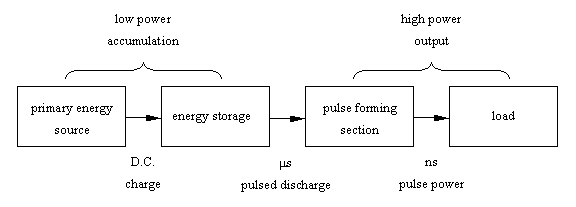
\includegraphics[height=4cm,width=8cm,keepaspectratio=true]{HPMsystem}
 \caption{Primjer ubacivanja slike.}
 \label{fig:prva}
	\end{center}
\end{figure}
\end{verbatim}
Uo�ite uporabu naredbe \verb|\label| unutar bloka. Na nju se potom u tekstu mo�emo referencirati pisanjem npr.\ \verb|Na Slici~\ref{fig:prva}| �ime \LaTeX{} u tekst uvrsti pripadaju�i broj slike, kao npr.\ ``Na Slici~\ref{fig:prva} prikazana je osnovna shema HPM sustava.''
Znak \verb|~| iza rije�i Slici osigurava to�no jedan znak razmaka, �to poma�e ukoliko je rije� Slika na kraju retka, da ne razdvoji rije� Slika i pripadaju�i broj slike.

\begin{figure}[!htbp]
	\begin{center}
 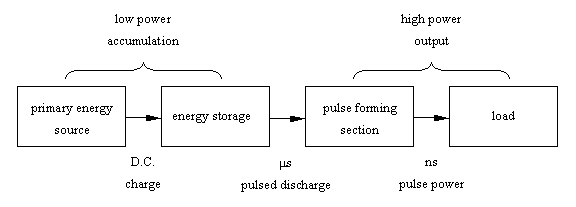
\includegraphics[height=4cm,width=8cm,keepaspectratio=true]{HPMsystem}
 \caption{Primjer ubacivanja slike.}
 \label{fig:prva}
	\end{center}
\end{figure}

Uo�ite i na�in prilago�avanja veli�ine slike. Parametri slike \emph{width} i \emph{height} odre�uju maksimalne dopu�tene dimenzije pri �emu se primarno po�tuje manju navedenu dimenziju, a \emph{keepaspectratio} osigurava zadr�avanje odnosa dimenzija slike, odnosno sprje�ava deformaciju slike, nakon proizvoljno unesenih veli�ina.

Uo�ite da sve oznake tj.\ \emph{labeli} ne smiju imati razmak u imenu. To vrijedi i op�enito, a ne samo za slike.

Tako�er, uo�ite da nije potrebno pisati ekstenziju slike jer to je ure�eno u postavkama glavnoga dokumenta pa time �tedi trud. Ekstenzije koje se mo�e izostaviti su: \emph{jpg}, \emph{jpeg}, \emph{png} i \emph{pdf}.

Shema prikazana na Slici~\ref{fig:prva} �e biti kori�tena i za potrebe idu�ih primjera, a {\color{blue} u mapi na va�em disku ju obri�ite nakon �to po�nete pohranjivati vlastite slike vezane uz va� rad}.


\section{Ubacivanje podslika}
Ponekada se jedna slika sastoji od dvije ili vi�e podslika kojima �elimo opisati neku cjelinu. Slika �e dobiti pripadni broj, a podslike slova (a), (b) itd.
To se mo�e posti�i sljede�om strukturom:
\begin{verbatim}
\begin{figure}[!htpb]
 \begin{center}
  \subfloat[Blok shema HPM sustava.]{\label{fig:HPM}
   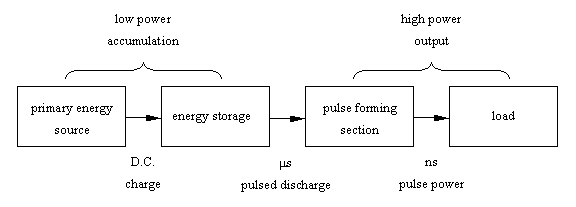
\includegraphics[height=5cm,width=10cm,keepaspectratio=true]{HPMsystem}}\\ 
	    %\hspace{10pt}
   \subfloat[JabRef su�elje za unos ``elektroni�ke'' reference.]
   {\label{fig:jabref}
   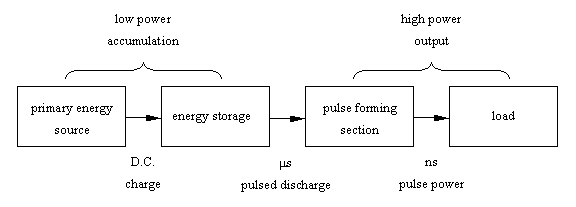
\includegraphics[height=7cm,keepaspectratio=true]{HPMsystem}}
\caption{Primjer ubacivanja vi�e podslika. Ovo je opis cijele slike.}
\label{fig:dvije_podslike}
  \end{center}
\end{figure}
\end{verbatim}
�to �e uvrstiti ono �to se vidi na Slici~\ref{fig:dvije_podslike}, koja se sastoji od dviju podslika.
Podslika~\ref{fig:HPM} pokazuje shemu HPM sustava, a podslika~\ref{fig:jabref} su�elje JabRef programa za unos bibliografskih jedinica.

\begin{figure}[!htpb]
	  \begin{center}
	   \subfloat[Blok shema HPM sustava.]{\label{fig:HPM} 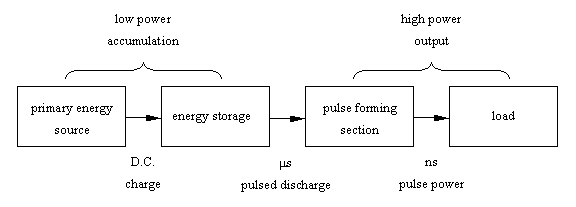
\includegraphics[height=5cm,width=10cm,keepaspectratio=true]{HPMsystem}} \\ %\hspace{10pt}
	   \subfloat[JabRef su�elje za unos ``elektroni�ke'' reference.]{\label{fig:jabref} 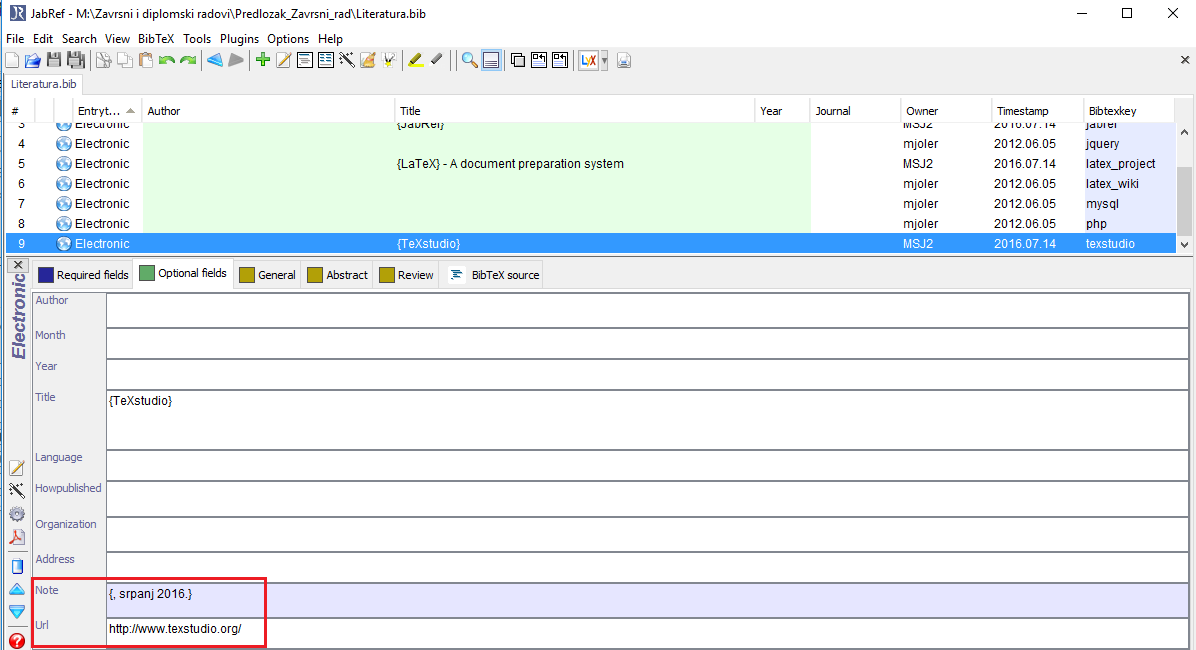
\includegraphics[height=7cm,keepaspectratio=true]{jabref}}
\caption{Primjer ubacivanja vi�e podslika. Ovo je opis cijele slike.}
\label{fig:dvije_podslike}
	  \end{center}
\end{figure}



\section{Ubacivanje tabele} 
Vi�e detalja o kreiranju tabela pro�itajte u literaturi, a sljede�i blok vam omogu�ava kreiranje jednostavne tabele, kao �to je prikazano u Tabeli~\ref{tab:prva}.
\begin{verbatim}
\begin{table}[!htbp]
\renewcommand{\arraystretch}{1.2}
\caption{Ovo je primjer izrade tabele.}
\centering
\begin{tabular}{|c|c|c|}
\hline
variabla & vrijednost 1 & vrijednost 2  \\ [0.5ex]
\hline \hline  
A & 5 & 3 \\ [0.5ex] % razmak do iducega retka
B & 4 & 2 \\ [0.5ex]
\hline
\end{tabular}
\label{tab:prva}
\end{table}
\end{verbatim}

\begin{table}[!htbp]
\renewcommand{\arraystretch}{1.2}
\caption{Ovo je primjer izrade tabele.}
\centering
\begin{tabular}{|c|c|c|}
\hline
variabla & vrijednost 1 & vrijednost 2  \\ [0.5ex]
\hline \hline 
A & 5 & 3 \\ [0.5ex] % razmak do iducega retka
B & 4 & 2 \\ [0.5ex]
\hline
\end{tabular}
\label{tab:prva}
\end{table}
%
Podaci koji su u stupcima se u tabeli razdvajaju znakom \&. Novi redak se na kraju aktualnoga retka formira znakom \verb|\\|. Broj stupaca se definira iza \emph{tabular} time �to se navedu slova koja ozna�avaju poravnavanje teksta u svakom stupcu, a broj slova zna�i broj stupaca koji �e biti kreiran u tabeli. Vertikalni razmak izme�u redaka u tabeli mo�ete za cijelu tabelu prilagoditi uporabom sljede�e sintakse prije strukture za tabelu:\\
\verb| \renewcommand{\arraystretch}{1.2} | gdje broj u zagradi na kraju (ovdje je 1.2) prilagodite sukladno va�oj preferenciji. Mo�e se prilagoditi i razmak za svaki pojedini redak (uo�ite \verb|[0.5ex]| na kraju redaka), ali to je manje od interesa jer tipi�no �elimo da svi retci imaju jednaki razmak jedni od drugih.

Sli�no mo�ete u�initi i za razmak izme�u stupaca tabele navo�enjem sljede�e sintakse prije bloka tabele:\\
\verb| \renewcommand{\tabcolsep}{0.3cm} |.



\section{Uporaba kratica u tekstu. Automatsko generiranje popisa kratica.}  \label{sec:kratice}
Listu kratica definirajte u datoteci \verb|Kratice.tex| (vidjeti predlo�ak unutar datoteke). U redovitom tekstu, kraticu  mo�ete ubaciti kori�tenjem naredbe \verb|\gls{ID_kratice}| gdje je \verb|ID_kraticE| identifikator kratice kako je definiran u datoteci \emph{Kratice.tex}. Pri prvoj uporabi naredbe \verb|\gls|, ispisat �e se najprije puni naziv pojma pa u zagradi kratica, a kod svake sljede�e uporabe, ispisat �e se samo kratica. Na primjer, kada (nakon prethodnog deklariranja u datoteci \verb|Kratice.tex|) upotrijebite \verb|\gls{gsm}| prvi puta, u tekstu �e se ispisati \gls{gsm}, a kada upotrijebite \verb|\gls{gsm}| drugi puta i dalje, u tekstu �e se ispisati samo \gls{gsm} (usporedi s definicijom kratice u datoteci \verb|Kratice.tex|). 
 
{\color{red} Listu kratica generirate sljede�im postupkom:} \label{generiranje_liste_kratica}
\begin{enumerate}
	\item Pokrenite kompilaciju cijeloga teksta jedanputa (to �e generirati neke datoteke koje su potrebne za daljnju obradu, specifi�no one s ekstenzijama .ist i .glo).
	\item Otvorite \emph{Command Prompt} aplikaciju na va�em ra�unalu i postavite se u radnu mapu gdje su vam datoteke za diplomski rad. 
	\item Potom pokrenite \emph{makeindex} rutinu (ona �e tipi�no biti ve� prisutna na va�em ra�unalu) upisuju�i sljede�u sintaksu: \\
	\verb|makeindex   -s myDoc.ist  -o myDoc.gls   myDoc.glo| \\
	gdje naziv datoteke \emph{myDoc} treba zamijeniti nazivom va�e glavne .tex datoteke, (npr. \verb|JMBAG_Ime_Prezime.tex|).
	\item Pokrenite \LaTeX{} jo� jednom ili dva puta, ako treba, dok se u uvodu pdf dokumenta ne pojavi lista kratica (pod naslovom \emph{Pojmovnik}).	
\end{enumerate}

Mo�da isprva zvu�i slo�eno, ali zapravo nije (bar ne uz ovako precizne upute!). Svaki puta kada dodate nove definicije kratica, potrebno je ponoviti ovaj postupak da bi se a�urirale odgovaraju�e datoteke i uredno prikazala potpuna lista u pdf-u (a i izbjegle poruke o pogre�kama tijekom kompajliranja teksta). 

Nije te�ko nakon �to prvi puta pro�ete ovaj postupak i omogu�ava vam u tekstu biti dosljedan u uporabi odre�ene kratice. Da izbjegnete �u�enje, va�no je jo� re�i da �e se ovim postupkom automatski stvoriti tek lista kratica koje ste u tekstu upotrijebili uporabom sintakse \verb|\gls|, a ne na temelju liste definicija koje ste naveli u datoteci \verb|Kratice.tex|. Zato, ako nijednom u tekstu ne upotrijebite sintaksu \verb|\gls|, ne�e biti ispisan ni popis kratica tj.\ \emph{Pojmovnik}. {\color{blue} Kako \LaTeX{} na kraju uvijek nagradi trud koji je ulo�en u savladavanje njegove sintakse, pogodnost ovakvoga automatskoga kreiranja Pojmovnika je i to �to uz svaki kraticu \LaTeX{} automatski ispi�e i brojeve stranica na kojima se doti�na kratica pojavljuje!} U elektroni�kom pdf dokumentu, brojevi stranica su ujedno i hiper-veze na te stranice pa se tako mo�e odmah sko�iti na stranicu gdje je pojedina kratica upotrijebljena.

Ukoliko vam se prethodno opisani postupak �ini preslo�enim, popis kratica mo�ete napraviti i ru�no, isto pomo�u datoteke Kratice.tex, u kojoj tako�er postoji kratki predlo�ak i za takav pristup. Za to je onda u osnovnoj datoteci \verb|JMBAG_Ima_Prezime.tex| potrebno deaktivirati liniju koda koja po�inje sa \verb|\printglossary|, a aktivirati blok koji po�inje sa \verb|\begin{glossary}| i zavr�ava sa \verb|end{glossary}|.



\section{Nagla�avanje teksta}
\subsection{Navodnici}
Za navodnike s lijeve strane fraze (otvaranje navodnika) koristi se 2x jednostruki navodnik koji se na tipkovnici nalazi lijevo od broja 1, a za navodnike s desne strane fraze (zatvaranje navodnika), koristi se 2x jednostruki navodnik koji se na tipkovnici nalazi na tipki \emph{�}, �to proizvede npr.\ ``abc''.

{\color{blue} Alternativno, u ovom paketu je pripremljena i naredba {\color{red} \verb|\navod{abc}|} gdje je \emph{abc} tekst koji se stavlja izme�u navodnika, tj.\ \navod{abc}.}

\subsection{Kosa i podebljana slova}
Nagla�avanje neke rije�i ili fraze pomo�u kosih (italic) slova mo�emo dobiti uporabom naredbe {\color{red} \verb|\emph{abc}|} ili pomo�u  {\color{red}\verb|\textit{abc}|} gdje je \emph{abc} neki tekst koji se �eli naglasiti.

\textbf{Podebljana slova} mo�emo posti�i uporabom naredbe {\color{red} \verb|\textbf{abc}|} gdje je \textit{abc} neki tekst koji �elimo podebljati.

\section{Verbatim: okru�enje za doslovni tekst}
Verbatim okru�enje omogu�ava ispis teksta u izvornom obliku, bez da ga \LaTeX{} tuma�i po svojiim sintakti�kim pravilima. To je pogodno kada se na stranicu  npr.\ �eli kopirati dio programskoga koda iz nekog jezika i kada �elimo zadr�ati sve izvorne znakove u nekoj frazi, bez da \LaTeX{} po�ne javljati pogre�ke kod kompajliranja, �to bi se moglo pojaviti kada se ne bi koristilo \emph{verbatim okru�enje}, po�to bi neke znakove interpretirao kao pogre�ke u sintaksi.

Postoji kra�i i du�i oblik verbatima. Kra�i slu�i za kra�u frazu od jedne ili par rije�i, a du�i za vi�e redaka.

\noindent Kra�i oblik verbatima ima sintaksu: \verb+\verb|neka fraza|+

\noindent Du�i oblik verbatima ima sintaksu:\\
\verb|\begin{verbatim}| \\
\verb|neki tekst| \\
\verb|\end{verbatim}| \\


\section{Kreiranje jedne jednad�be ili serije jednad�ba}

\subsection{Kreiranje jedne jednad�be}
Jednad�ba se napi�e u posebnom matemati�kom modu koji se kreira pomo�u bloka:
\begin{verbatim}
	\begin{equation}
		 A = B + C   \label{eq:prva}
	\end{equation}
\end{verbatim}
�to �e dati sljede�i izgled:
\begin{equation}
	 A = B + C   \label{eq:prva}
\end{equation}
Da bi se na nju referenciralo, na �eljenom mjestu u tekstu upi�emo \verb|\eqref{eq:prva}|, �ime �e se uvrstiti njezin pripadni (automatski generirani) broj, a za potpuniji smisao mo�emo npr.\ napisati \verb| Jednad�ba~\eqref{eq:prva}|, rezultat �ega je da �e u tekstu pisati Jednad�ba~\eqref{eq:prva}. 
Ako ju se ne �eli numerirati, onda se nakon rije�i \emph{begin} stavi zvjezdica, tj.\ \verb|begin*{equation}|.

\subsection{Kreiranje grupe jednad�ba}
Grupa jednad�ba se kreira uporabom \emph{subequations} sintakse. Na primjer, sljede�i blok �e definirati dvije podjednad�be u grupi, gdje �e svaka biti numerirana istim brojem, a razlikovati slovom iza broja.
\begin{verbatim}
	\begin{subequations}
		\begin{align}
		        A &= B + C  	\label{subeq:prva} \\
		        D &= F + G		\label{subeq:druga}
		\end{align}
	\label{subeq:obje}
	\end{subequations}
\end{verbatim}

To �e u izlaznom dokumentu rezultirati sljede�im izgledom:
\begin{subequations}
\begin{align}
        A &= B + C  	\label{subeq:prva} \\
        D &= F + G		\label{subeq:druga}
\end{align}
\label{subeq:obje}
\end{subequations}
U \eqref{subeq:prva} je prikazano dobivanje vrijednosti $A$, a u \eqref{subeq:druga} je prikazano dobivanje vrijednosti $D$. Jednad�ba~\eqref{subeq:obje} je \emph{�uveni studentov zakon}!



\section{Liste}
Liste su �este forme u tekstu kojima se na pregledni na�in nabrajaju neke stavke. Stavke obi�no navodimo ili s to�kama na po�etku, s brojevima ili sa slovima. U \LaTeX-u su upravo ta tri stila unaprijed definirana, a mogu�e su i slo�enije definicije stilova i kombinacije lista.

\subsection{Lista s to�kama}
Lista s to�kama se postigne blokom
\begin{verbatim}
\begin{itemize}
    \item prva nenumerirana stavka
    \item druga nenumerirana stavka
\end{itemize}
\end{verbatim}
�to na ekranu proizvede:
\begin{itemize}
% \setlength\itemsep{1ex}   % za lokalnu prilagodbu
	\item prva nenumerirana stavka
	\item druga nenumerirana stavka
\end{itemize}

\subsection{Lista s brojevima}
Numerirana lista s brojevima se postigne blokom
\begin{verbatim}
\begin{enumerate}[itemsep=1ex, topsep=4pt, partopsep=0pt]
     \item prva numerirana stavka
     \item druga numerirana stavka
\end{enumerate}
\end{verbatim}
U uglatoj zagradi su tri parametra kojima se to�no mo�e kontrolirati vertikalni razmak izme�u stavki u listi (\emph{itemsep}), razmak izme�u prethodnoga teksta i prve stavke u listi (\emph{topsep}) i dodatni prostor izme�u liste i prethodnoga paragrafa kada lista zapo�inje novi paragraf (\emph{partopsep}), ali te parametre \textbf{ne morate navoditi} tj.\ tu uglatu zagradu ne morate pisati. Tada �e se primijeniti vrijednosti parametara koje su definirane za cijeli dokument, a ove parametre se mo�e upotrijebiti tek da u nekom pojedinom slu�aju prilagodite razmake.
Za osjetiti efekte ovih parametara, najbolje se malo sam poigrati razli�itim vrijednostima parametara i vidjeti posljedice toga na listu (pri tome se uz brojeve kao prikladne jedinice za razmak mogu koristiti \emph{pt}, \emph{ex} ili \emph{em}).

\subsection{Proizvoljno ozna�ena lista}
Takva se lista mo�e posti�i u sklopu op�enitije forme koja omogu�uje proizvoljni opis ispred pojedine stavke, pomo�u sljede�ega bloka:
\begin{verbatim}
\begin{description}
     \item[a)] prva opisna stavka
     \item[b)] druga opisna stavka
\end{description}
\end{verbatim}
�to na ekranu proizvede:
\begin{description}%[itemsep=1ex, topsep=4pt, partopsep=0pt] za lokalnu prilagodbu
	\item[a)] prva opisna stavka
	\item[b)] druga opisna stavka \\
\end{description}
%
Kod ove strukture, u uglatu zagradu iza naredbe \verb|\item|, navodi se proizvoljna oznaka kojom se �eli na neki na�in ``numerirati'' listu.
%:::::::::::::::::::::::::::::::::::::::::::::::::::
\chapter{Dodatne informacije}
\section{Primjeri uporabe sintakti�kih struktura}
\begin{enumerate}
	\item Za uvid u kontekstualnu primjenu raznih sintakti�kih struktura, mo�ete otvoriti datoteku \href{run:Intro.tex}{{\color{blue}Intro.tex}}, unutar koje su napisane i ove upute. 
	\item Primjere slo�enijih sintakti�kih struktura, kao �to su ubacivanje slike, tabele ili jednad�be, mo�ete na�i u datoteci \href{run:sintaksa_cestih_struktura.tex}{{\color{blue}sintaksa\_cestih\_struktura.tex}} koja je dio paketa. Odabrane se strukture mo�e kopirati i zalijepiti u va� tekst, uz minimalne prilagodbe kao �to su naziv slike, veli�ina slike, opis i ID slike, a analogno i za tabele i jednad�be.
	\item Kona�no, za vi�e detalja o bilo �emu, potra�ite informacije u dvama priru�nicima koji su prilo�eni u mapi \href{run:prirucnici}{{\color{blue}prirucnici}} ili na webu, gdje se, me�u obiljem drugih informacija, nalaze i korisne wiki stranice \cite{latex_wiki,tex_exchange} o \LaTeX-u pomo�u kojih se obi�no brzo prona�e upute i zadovoljavaju�e rje�enje kakvom sintaksom se mo�e urediti �eljeni dio teksta.
\end{enumerate}

\section{Savjeti za lak�e ure�ivanje teksta}
Vjerujem da vam ovaj dokument mo�e uvelike pomo�i u pripremi teksta va�ega zavr�nog/diplomskog rada i omogu�iti da glavninu vremena tro�ite na sadr�aj rada, a manje na formatiranje rada jer to �e za vas sada obaviti \LaTeX{}! 

No, korektnosti radi, potrebno je napomenuti i sljede�e: \LaTeX{} je vrlo osjetljiv na pogre�ke u sintaksi naredbi (da, ba� kao �to su i programski jezici) pa vas mo�e povremeno ugnjaviti javljanjem pogre�ke koju nikako ne uspijevate uo�iti gdje je. Iskustvo kojim se izbjegava ta nelagoda jest sljede�e:
\begin{itemize}
	\item svako poglavlje napi�ite u novoj datoteci (da biste koli�inu teksta razdvojili na preglednije i manje cjeline) koju imenujte prikladnim imenom (bez razmaka u imenu). Potom te datoteke samo pozivajte iz glavnoga dokumenta \verb|JMBAG_Ime_Prezime.tex| pomo�u naredbe \verb|\include{ime_datoteke}|. Takav je pristup upravo i kori�ten u pripremi ovoga paketa.
	%
	\item {\color{red} budite koncentrirani dok pi�ete \LaTeX{} naredbe, poglavito zagrade, posebne znakove i matemati�ki tekst gdje se zahtijeva uporaba znaka \$!}
	%
	\item kompajlirajte tekst prije nego se skupi puno teksta jer tako �ete imati manje teksta za prekontrolirati u slu�aju pogre�ke. Tako�er vam za provjeru tek manjega dijela dokumenta mo�e pomo�i paket \verb|\usepackage{syntonly}| i naredba \verb|syntaxonly|, a isto tako i naredba \verb|\includeonly{ime_datoteke}| kojom �ete kompajlirati samo tu navedenu datoteku, �ime  ispred ``ne�eljenih'' datoteka ne morate stavljati znak ``komentara'' (\%).
	%
	\item ako niste sigurni ho�e li vam raditi neka naredba nakon pisanja, radije tekst kompajlirajte odmah po pisanju te naredbe---da vidite �to �ete dobiti i rije�ite dvojbu, nego da �ekate da se skupi jo� dubioznih mjesta u tekstu, kada �e nakon kompajliranja biti te�e detektirati koja linija teksta zapravo izaziva probleme (\LaTeX-ov prozor s porukama �esto nije odve� precizan u lociranju i opisu pogre�aka, ovisno o editoru teksta koji koristite).
\end{itemize}


\section{Zavr�ne napomene}
Ovime zaklju�ujemo uvodne upute koje �e najve�em broju studenata biti dovoljne (ili barem dovoljna osnova) za uspje�no pisanje zavr�nog odnosno diplomskog rada.

Prije nego prije�ete na kreiranje vlastitoga sadr�aja u�inite jo� sljede�e akcije kojima �ete deaktivirati dio paketa koji �e biti nepotreban:
\begin{enumerate}
	\item u mapi \href{run:slike}{{\color{blue}slike}}, obri�ite datoteke \verb|HPMsystem.png| i \verb|jabref.png| jer su one slu�ile tek za ilustracije u ovim Uputama.
	%
	\item u glavnoj datoteci  \href{run:JMBAG\_Ime\_Prezime.tex}{{\color{blue}JMBAG\_Ime\_Prezime.tex}} stavite znak komentara ``\%'' ispred linije \verb|\chapter{Kako koristiti paket za pisanje zavr�noga rada u \LaTeX-u}
Ovo su uvodne napomene za kori�tenje predlo�ka za pisanje zavr�noga ili diplomskoga rada studenata Tehni�koga fakulteta u Rijeci. Prije kori�tenja paketa, pro�itajte ovaj tekst jer �e vam dati nu�ne uvodne informacije, znatno vam olak�ati i ubrzati ure�ivanje teksta nakon toga, pri �emu �e vas i voditi kroz uporabu ovoga paketa na prakti�an na�in.

Paket je pripremljen tako da student �to prije mo�e pisati vlastiti tekst u ve� pripremljenom predlo�ku koji �e, uz minimalno u�enje sintakse \LaTeX-a, studentu olak�ati urediti svoj rad. U paketu su uklju�ene potrebne upute i sintakti�ke strukture koje bi trebale udovoljiti potrebama ve�ine studenta, a dodatne informacije postoje u dvama priru�nicima koji su uklju�eni u ovom paketu te, naravno, na raznim web stranicama na internetu koje su posve�ene \LaTeX-u (vidi u nastavku).

{\color{red} POZOR: paket treba biti prekopiran negdje na disk ne mijenjaju�i originalnu strukturu mapa (foldera) i ne mijenjaju�i nazive datoteka koje su u mapi \emph{tex\_aux}!}


\section{Opis sadr�aja paketa}
\vspace{-2ex}
Paket se sastoji od:
\begin{itemize}
 \item datoteke \href{run:UPUTE.pdf}{{\color{blue} UPUTE.pdf}} koja sadr�i postupak instalacije potrebnih alata na ra�unalo te kori�tenja paketa. \emph{UPUTE} su bazirane na Windows OS, a korisnici drugih OS-ova si na nazna�enim web lokacijama samo trebaju na�i instalacije za njihov OS.
 %
 \item datoteke \verb|JMBAG_Ime_Prezime.tex| koja je sredi�nja datoteka koja povezuje sve cjeline i kompajliranjem koje se dobije izlazni \verb|JMBAG_Ime_Prezime.pdf| dokument (naravno, tijekom rada, upisat �ete svoj specifi�ni JMBAG i ime i prezime).\\ U ovoj se datoteci inicijalno nalaze i upute za kori�tenje paketa kao i primjeri osnovne uporabe naj�e��ih sintakti�kih struktura u \LaTeX-u koje bi trebale biti dovoljne ve�ini studenata za pisanje rada.
 %
 \item mape \verb|tex_aux| u kojoj su \emph{interne datoteke} koje definiraju stilove, formate i sl.\ koji slu�e u slaganju izlaznoga formata. \textbf{Student/ica s njima ne treba \emph{ni�ta} raditi}, ali one trebaju biti u \verb|tex_aux| mapi pod glavnom mapom zavr�noga rada, kao �to je postavljeno u ovom paketu.
 %
 \item mape \emph{slike} u koju student treba pohraniti sve slike koje �e koristiti u radu. Ime mape se ne smije preimenovati bez boljega poznavanja sintakse \LaTeX-a jer ovaj paket da bi ispravno radio o�ekuje ba� takvo ime mape!
 %
 \item datoteke \verb|sintaksa_cestih_struktura.tex| koja ne sudjeluje izravno u kompajliranju pdf dokumenta, nego slu�i kao repozitorij u kojemu su sadr�ane naj�e��e potrebne sintakti�ke strukture koje su spremne za kopiranje u va� tekst uz minimalnu prilagodbu parametara (npr.\ opis slike, ime datoteke specifi�ne slike koju se ubacuje i proizvoljni ID te slike za kasnije referenciranje).
 %
 \item mape \href{run:prirucnici}{{\color{blue}prirucnici}} u kojoj se nalazi nekoliko najpopularnijih priru�nika za uporabu \LaTeX-a. 
\end{itemize}
%%%%%%%%%%%%%%%%%%%%%%%%%%%%%%%%%%%%%%%%%%%%%%%%%%%%%%%%%%%%%%%

\section{�ime se opremiti za pisanje rada}
Da bi se rad napisao pomo�u \LaTeX-a (a to vrijedi svake lipe!), najprije je na ra�unalo potrebno instalirati:
\begin{enumerate}
	\item obavezno: \LaTeX{} software 
	\item obavezno: editor za ure�ivanje teksta 
	\item neobavezno, ali korisno: softver za opis literature. (Premda dodatni softver nije nu�an jer se popis literature mo�e obraditi i ru�no (no to je manje sofisticirano kod uvr�tavanja referenca), sugeriram instalaciju softvera koji pomo�u intuitivnih su�elja korisniku omogu�ava opis pojedine kori�tene literature (kao mala baza podataka), a potom se pojedina jedinica literature jednostavno ubacuje u tekst, a popis literature se na kraju automatski formira (vi�e o tome pro�itajte u nastavku).
\end{enumerate}

\subsection{Instalacija \LaTeX-a}
\begin{enumerate}
	\item odite na sredi�nji \LaTeX{} portal \cite{latex_project}: \url{http://www.latex-project.org/}
	\item kliknite na poveznicu \href{http://www.latex-project.org/ftp.html}{Getting LaTeX} i potom uo�ite i povucite instalaciju koja odgovara va�em OS-u (npr.\ proTeXt za Windows, MacTeX za Mac, TeX Live za Linux). Pozor: instalacijski paket je velik i mo�e du�e potrajati �ak i na brzoj vezi---dajte si dovoljno vremena za obaviti download.
	\item Instalirajte \LaTeX{} slijede�i upute koje su prilo�ene za odabranu instalaciju (npr.\ proTeXt za Windowse daje kratki pdf s uputama koje vas vode kroz instalaciju korak po korak).
\end{enumerate}

\subsection{Instalacija editora teksta}
Instalirajte editor koji je pogodan za pisanje \LaTeX{} koda. \textbf{Za Windows OS, toplo preporu�am}  \href{http://www.texstudio.org}{{\color{blue} TeXstudio}} \cite{texstudio} jer je bogat opcijama, ugodan za rad i stabilan, a instalacije postoje i za Linux i Mac OS. TeXstudio se zasebno povu�e i instalira na ra�unalo, a neke editore teksta koji ve� do�u u paketu za instalaciju LaTeXa mo�ete ignorirati (npr.\ za Windows je do nedavno bio popularan \emph{TeXnicCenter} i dolazi ve� upakiran u proTeXt-u (a mo�da �ete na�i i \emph{TeXworks}), za Mac je kvalitetan \emph{TeXShop} koji sada tako�er dolazi u paketu s MacTeX-om). 

\label{encoding1} {\color{red} POZOR: Premda �e ovo biti jo� napomenuto na stranici~\pageref{encoding2}, prije samoga po�etka pisanja va�ega rada, �to prije �elim napomenuti sljede�i va�ni detalj: za svaki va� tekst koji pi�ete u editoru teksta, uvjerite se da je kodna stranica postavljena na \navod{windows-1250}, �to je klju�no da bi se u izlaznom pdf-u ispravno ispisivali hrvatski dijakriti�ki znakovi! U TeXstudiu, aktualnu kodnu stranicu se mo�e vidjeti i promijeniti preko maloga izbornika u doljnjem desnom kutu glavnoga prozora, gdje se nalazi opcija ``Encoding''. Ukoliko tu ne pi�e ``windows-1250'', kliknite na izbornik, odaberite opciju ``More Encodings'' pa u potom otvorenom su�elju odaberite kodnu stranicu ``windows-1250 / CP 1250'' i potvrdu sa ``Change To''.}

\subsection{Instalacija programa za opis kori�tene literature}
\emph{Ponavljamo: Kori�tenje BiBTeX programa za opis literature \textbf{nije} neophodno, ali jest korisno. U datoteci po imenu \href{run:Literatura.tex}{{\color{blue}Literatura.tex}}, koja je uklju�ena u ovaj paket, ve� su namje�tene postavke kao da �e se literatura opisati pomo�u BiBTeX programa (npr.\ JabRef-a) i ne treba ni�ta mijenjati, ali ispod toga se mo�e prona�i i upute i za drugi--ru�ni-- na�in (p)opisivanja literature.}

Kao bibtex program za opis literature, preporu�am \href{http://www.jabref.org}{{\color{blue} JabRef}} program \cite{jabref}. To je legalno besplatno dostupni program za Windows OS (ali postoji i za Mac, a i platformski neovisna instalacija) koji nam omogu�ava opisivanje literature na lak na�in pomo�u intuitivnih su�elja, a kao rezultat kreira \emph{BibTeX} datoteku \emph{Literatura.bib} (gdje je (\emph{Literatura} naziv koji korisnik treba dodijeliti pri pohrani JabRef datoteke na disk u slu�aju ovoga predlo�ka, da bi paket funkcionirao) u kojoj je literatura opisana na na�in koji \LaTeX{} razumije. 

Uo�ite da ako ne koristite JabRef, ve� se odlu�ite za ru�ni unos literature, �to se isprva doima jednostavnijim, tada �e vam redoslijed referenca u popisu literature odgovarati to�no redoslijedu koji ste naveli u tom popisu --- dakle morate paziti da redoslijed formirate onim redom kojim pozivate reference u va�em tekstu (�to kod nekog kasnije ubacivanja dodatne reference unutar ve� postoje�ega redoslijeda tra�i brigu da ju se ubaci na odgovaraju�e mjesto u popisu literature), a tako�er trebate paziti i na formatiranje teksta svake reference! 

Za razliku od toga, kori�tenjem JabRef-a, izbjegavate ru�no formiranje popisa literature i ne trebate brinuti o redoslijedu referenca, ve� samo pomo�u JabRefa trebate unijeti sve jedinice literature koju �ete navesti, a \LaTeX{} �e vam automatski formirati listu referenca onim redoslijedom kojim reference bude pozivali u tekstu!

Nakon �to kompajlirate projekt, stvorit �e vam se pomo�na datoteka imena \href{run:JMBAG_Ime_Prezime.bbl}{{\color{blue}JMBAG\_Ime\_Prezime.bbl}} u kojoj �e jedinice literature tijekom kompilacije biti formatirane i odatle se ubacuju u kona�nu verziju teksta. Stoga, \textbf{ukoliko ima ikakvih detalja koje u opisu literature treba prilagoditi, a ne mo�ete automatskim putem}, uvijek vam kao ``zadnja crta obrane'' ostaje otvoriti \verb|bbl| datoteku i tamo ru�no napraviti izmjene. Potom ponovo kompajlirajte projekt i te �e se promjene vidjeti u pdf-u tj.\ ru�no unijete promjene ne�e biti poni�tene sve dok ne obri�ete cijelu datoteku.

Umjesto da rukom pi�ete cijelu bibliografiju, vremenski vam je vjerojatno u�inko\-vitije popis literature generirate uporabom JabRef-a, a potom ako i�ta jo� treba prilagoditi, onda samo to napraviti ru�no u \verb|bbl| datoteci.


\subsubsection{Osnovna uporaba JabRef programa}
Upoznajte se s najva�nijim opcijama u \emph{JabRef}-u:
\begin{itemize}
	\item uo�ite ikonu (pod znakom ``+'' i tekstom \emph{New BibTeX Entry}) za unos nove jedinice literature (npr. knjige, �lanka, web portala i sl.)
	%
	\item kada kliknete za unos nove stavke literature, uo�ite kakvi se sve tipovi literature nude za odabir. Odabirom opcije koja odgovara naslovu koji �elite unijeti, otvorit �e vam se novi prozor s poljima u koja se mo�e unijeti informacije o literaturi. Za odabrani tip literature samo su neka polja obavezna (nalaze se pod karticom (eng.\ \emph{tabom}) \emph{Required fields}), dok se pod drugim karticama mo�e i ne mora unijeti dodatne informacije. U slu�aju na�ih zavr�nih/diplomskih radova, bit �e znatan udjeli literature koja je na internetu pa za formatiranje iste, pro�itajte upute i napomene u nastavku ove sekcije.
	%
	\item kada je vi�e autora, njihova imena se u JabRefu polju za unos autora razdvajaju pisanjem klju�ne rije�i \verb|and| (a ne razmakom, zarezom ili to�ka-zarezom!)
	%
	\item U popisu literature se ne�e uvijek pojam prepisati onako kako ste ga vi zapisali u JabRefu! To je posljedica stilova koji su definirani u \verb|bst| datoteci (ne zamarajte se time sada jer je za naprednu razinu \LaTeX-a). No, ako neki pojam ba� ne ispadne suvislo napisan u popisu literature ili ba� �elite forsirati odre�eni na�in zapisa (�esto slu�aj kada se rije� s velikim slovima ne interpretira onako kako �elite), tada to�no odre�eni zapis mo�ete forsirati na na�in da \verb|{tu rije� ili frazu stavite unutar viti�astih zagrada}|
	%
	\item prije nego pohranite pojedinu stavku pomo�u \emph{Ctrl+S}, \textbf{morate svakoj jedinici literature dodijeliti jedinstveni identifikator}, tzv.\ \emph{Bibtexkey}, �to je jedno od polja koja su obavezna za unos. Mo�ete ru�no upisati neki proizvoljni string, ali pogodnije je generirati ga automatski.\\ Za to u�initi me�u ikonama na vrhu imate ikonu koja izgleda kao (�arobni) �tapi� sa zvjezdicama oko njega, klikom na kojega \emph{JabRef} automatski dodijeli jedinstveni BibTeX \emph{klju�} za tu bibliografsku jedinicu. Pomo�u toga klju�a se poslije bilo kada i bilo gdje u pisanju va�ega rada mo�ete pozvati na tu referencu, a \LaTeX{} �e sve ostalo obaviti za vas tj.\ dodijeliti joj odgovaraju�i broj u tekstu i s tim brojem uvrstiti u popis literature.
	%
	\item korisnik ima mogu�nost i promijeniti uzorak po kojem se kreira struktura automatski generiranoga jedinstvenoga BibTeX klju�a tako da se otvori opcija izbornika \emph{Options $>>$ Preferences $>>$ BibTeX key generator}, gdje je na vrhu prozora prikazan \emph{default} uzorak, npr. \verb|[auth]:[year]| �to zna�i da se klju� kreira na bazi \verb|prezime(autora):godina(rada)|. To se sada mo�e urediti po nekom novom uzorku, no ovako definirani uzorak u biti zadovoljava, a ako igdje ima potrebe za dodatnim razlikovanjem, mo�e se na automatski generiranom klju�u jo� ru�no napraviti korekcija dodavanjem nekog znaka na kraju, kao npr.\ dodavanjem \verb|_a| i sl. (Klikom na karticu \emph{BibTeX source} mo�ete vidjeti kako �e unos va�ih podataka zapravo biti zapisan u va�oj \emph{Literatura.bib} datoteci koja �e se formirati od svih bibliografskih jedinica koje unesete.)
	%
	%
	\item Za \emph{ime} va�e bibliografske datoteke kod pohrane na disk obavezno upi�ite  \emph{Literatura} jer to ime o�ekuje ovaj paket. Pozor: Datoteka \emph{Literatura.bib}, koju ste tako kreirali, mora se nalaziti unutar mape ovoga paketa da bi sve ispravno radilo! U paketu je za primjer ve� kreirana jedna datoteka istoga imena koju za vje�bu student mo�e i otvoriti u \emph{JabRef}-u, ali to su samo pokazne bibliografske jedinice unesene kao primjer, koje student treba u kona�nici zamijeniti svojim bibliografskim jedinicama.
	%
	\item Za ``elektroni�ke'' izvore literature (tj.\ sve �to ste kao informaciju na�li na webu), JabRef nudi tip literature pod nazivom ``Electronic'' (vidi Sl.~\ref{fig:jabref}). U njemu pod karticom (eng.\ tabom) \emph{Optional fields} pod poljem \verb|Title| mo�ete upisati ime web stranice (autor, tvrtka i sl.), pod poljem \verb|url| mo�ete upisati URL adresu te web stranice, a pod poljem \verb|Note| upisati datum kada ste posjetili tu web stranicu (npr.\ \emph{srpanj 2016.} ili \emph{3.~rujna~2016.}). Rezultat toga �e u pdf-u biti da je sve napisano redoslijedom koji je predvi�en u Uputama RiTeha za pisanje diplomskog rada \cite{riteh_upute}, \emph{osim �to u ovom Predlo�ku do sada nisam uspio rije�iti ubacivanje zareza izme�u URL adrese i datuma posjeta toj URL adresi}, koji bi ta dva podatka odvojio, pa je tu potrebna mala ru�na \emph{prilagodba na jedan od ovih dvaju na�ina}:
	\begin{enumerate}[label=\textbf{\roman*)}]
		\item kod unosa datuma u polje \verb|Note| (u su�elju JabRef-a), upi�ite datum na sljede�i na�in: \verb|{, <datum>}|, gdje je \verb|<datum>| va� specifi�ni datum, dok �e \emph{zarez} iza prve zagrade izvr�iti razdvajanje URL adrese i datuma, a \textbf{viti�aste zagrade} osigurati da se to ba� tako to�no prenese u pdf-dokument (uklju�uju�i i da se mjesec napi�e malim po�etnim slovom, �to ina�e ne bi bio slu�aj). (Za neke druge tipove referenca kao npr.\ tip \emph{manual}, zarez vam prije datuma ne�e trebati jer �e naziv literature zavr�iti zarezom.) U Jabrefu vam i ina�e vrijedi da kada �elite forsirati da se pojam ba� to�no u popisu literature zapi�e onako kao ste htjeli, onda se pojam stavi unutar viti�astih zagrada \verb|{kao u ovom primjeru}|.
		\item ako u polju \verb|Note| ne upi�ete datum na prethodno opisani na�in, onda vam u pdf dokumentu ne�e biti upisan zarez izme�u URL adrese i datuma koji ste unijeli, a tako�er �e i mjesec biti napisan velikim po�etnim slovom (�to nije stra�no, ali je manje po�eljno). To mo�ete \emph{ru�no} prilagoditi tako da otvorite \verb|.bbl| datoteku i pomo�u \emph{Find/Replace} operacije sve nazive mjeseca zamijenite na na�in da po�inju malim po�etnim slovom (�to nije te�ko kada vam je ve�ina datuma u popisu literature navedena u istom mjesecu), ali zareze �ete svakako morati ubacivati ru�no u svaku pojedinu stavku literature jer ne�e biti nekog predlo�ka kojim biste to rije�ili automatski pomo�u \emph{Find/Replace} operacije. Na kraju opet kompajlirajte projekt. S obzirom na navedeno, prvi na�in je vremenski �tedljiviji!
	\end{enumerate}
\end{itemize}

%%%%%%%%%%%%%%%%%%%%%%%%%%%%%%%%%%%%%%%%%%%%%%%%%%%


\chapter{Primjeri naj�e��ih sintakti�kih struktura}
Prije stvarnoga po�etka pisanja svoga rada, upoznajte se s osnovnim sintakti�kim strukturama koje �e vam trebati tijekom pisanja rada.

U nastavku su opisane naj�e��e sintakti�ke strukture (dio njih mo�ete na�i i u datoteci \emph{Intro.tex}), a dodatne slo�enije strukture su pohranjene u datoteci \href{run:sintaksa_cestih_struktura.tex}{{\color{blue}sintaksa\_cestih\_struktura.tex}} koja je sastavni dio glave mape ovoga paketa. 

\section{Postavljanje naslova poglavlja i sekcija}
\begin{itemize}
	\item \verb|\chapter{Naslov poglavlja}|: za definiranje naslova poglavlja
	\item \verb|\section{Naslov sekcije}|: za definiranje naslova sekcije unutar poglavlja
	\item \verb|\subsection{Naslov podsekcije}|: za definiranje naslova podsekcije
\end{itemize}


\section{Reference na literaturu} \label{sec:RefLit}
Za referencu na pojedini kori�teni izvor informacije (tj.\ jedinicu literature), koristimo naredbu \\
\verb|\cite{bibtexkey}|, gdje je \emph{bibtexkey} jedinstveni klju� kojim prethodno ozna�imo tu jedinicu literature. \verb|Bibtexkey| mo�emo definirati na jedan od sljede�ih na�ina:
\begin{description}
	\item[I)] ako popis literature definiramo izravno u datoteci \href{run:Literatura.tex}{{\color{blue}Literatura.tex}} (opcija (I) u datoteci), onda ispred svake stavke literature treba definirati i jedinstveni \verb|bibtexkey| pomo�u naredbe \verb|\bibitem{bibtexkey}| (vidi predlo�ak u datoteci)
	\item[II)] ako literaturu opisujemo pomo�u JabRef datoteke \emph{Literatura.bib} (opcija (II) u datoteci), onda se tamo uz svaku stavku definira \verb|bibtexkey| (bude na dnu JabRef obrasca za upis pojedine jedinice literature)
\end{description}
%
Npr.\ ako negdje u tekstu napi�emo \verb|\cite{latex_wiki}|, gdje je \verb|latex_wiki| prethodno definirani \emph{bibtexkey}, tada �e se u tekstu u uglatoj zagradi pokazati broj  te bibliografske jedinice pod kojim se nalazi u popisu literature (Bibliografiji) na kraju rada (u ovom primjeru, to je broj \cite{latex_wiki}).


\section{Referenca na sekciju, sliku, tabelu ili stranicu} \label{sec:RefText}

Za referenciranje na pojedine dijelove teksta unutar rada, koristimo
{\color{red} \verb|\label{ID}|} i {\color{red} \verb|\ref{ID}|} na na�in da se \verb|\label{ID}| postavi uz dio teksta koji �elimo ozna�iti internom oznakom i poslije �emo se u tekstu na to referencirati, a \verb|\ref{ID}| upotrijebimo na mjestu s kojega se referenciramo na dio teksta koji je ranije ozna�en pomo�u \verb|\label{ID}|.

Ako se �elimo referencirati na specifi�nu sliku ili tabelu ili sekciju ili jednad�bu u tekstu, tada unutar bloka toga sadr�aja stavimo oznaku \verb|\label{prefiks:ID_objekta}| gdje je \emph{objekt} slika ili tablica ili sekcija teksta ili jednad�ba, a na �eljenom mjestu u tekstu se na to referiramo pomo�u \verb|\ref{prefiks:ID_objekta}| (u slu�aju referenciranja jednad�be, bolji oblik naredbe je {\color{red} \verb|\eqref{prefiks:ID_objekta}|}).

\verb|ID_objekta| je proizvoljni string (bez razmaka) koji dodijelimo objektu od interesa, a radi preglednijega ure�ivanja teksta, uobi�ajeno je u \LaTeX-u za pojedine tipove oznaka staviti i odgovaraju�i \emph{prefiks}, kao npr.\ \emph{sec} za oznaku sekcije, \emph{fig} za oznaku slike, \emph{tab} za oznaku tabele, \emph{eq} za oznaku jednad�be i sl. (Tako bi za sliku kojoj dodijelimo $ID=prva$ bilo \verb|\label{fig:prva}|, za tablicu \verb|\label{tab:prva}|, za sekciju \verb|\label{sec:prva}|, a za jednad�bu \verb|\label{eq:prva}|.)

Za referencirati se na \emph{stranicu} u tekstu gdje se nalazi ne�to na �to se �elite osvrnuti, koristi naredba {\color{red} \verb|\pageref{prefiks:ID_objekta}|}. Za njenu primjenu se tako�er prethodno treba ozna�iti �eljeni tekst pomo�u naredbe \verb|\label|.

Tako npr.\ mo�emo staviti da je primjer kreiranja tabele \emph{prva} opisan na stranici~\verb|\pageref{tab:prva}|, �to �e za rezultat imati tekst u kojem pi�e ``da je primjer kreiranja tabele \emph{prva} opisan na stranici~\pageref{tab:prva}'' (jer se u tekstu ta tabela nakon kompajliranja npr.\ na�e na stranici 12). Kako god se tekst smanjivao ili pove�avao i navedena tablica mijenjala broj stranice na kojoj se u kona�nici nalazi, mi ne moramo o tome brinuti jer \LaTeX{} brine o tome i na kraju napi�e to�ni broj stranice! (To je jo� jedna o pogodnosti zbog �ega se ljudi i odlu�e, uz ne�to po�etnoga truda, za kori�tenje \LaTeX-a!).



\section{Poveznica na neki dokument ili URL adresu}
Naredbe \verb|\url| i \verb|\href| slu�e za kreiranje poveznice na neku URL adresu ili neki dokument na disku.

{\color{red}\verb|\url{adresa}|} �e otisnuti URL adresu to�no onako kako je \emph{adresa} navedena unutar zagrada.

{\color{red}\verb|\href{akcija:destinacija}{opis}|} �e na papiru/ekranu ispisati tekst \emph{opis} koji je naveden u drugoj zagradi, i izvr�iti \emph{akciju} prema \emph{destinaciji} koja je navedena u prvoj zagradi. 
\emph{Akcija} mo�e npr.\ glasiti \emph{run} ili \emph{mailto}, gdje �e prvi oblik otvoriti mapu ili datoteku staza koje je navedena kao \emph{destinacija}, a drugi oblik pokrenuti pisanje emaila prema email adresi koja je navedena kao \emph{destinacija}.

Ne pretjerujte ipak s uporabom ovih struktura, odnosno uop�e ne morate to koristiti u radu, nego za vanjske reference koristiti samo \verb|\cite{bibtexkey}| naredbu, a za unutra�nje reference (na dijelove teksta) kombinaciju naredbi \verb|\label{ID}| i \verb|\ref{ID}| kako je to opisano u Sekciji~\ref{sec:RefText}. 


\section{Ubacivanje slike}
Sliku mo�emo ubaciti pomo�u sljede�ega bloka naredbi:
\begin{verbatim}
\begin{figure}[!htbp]
	\begin{center}
 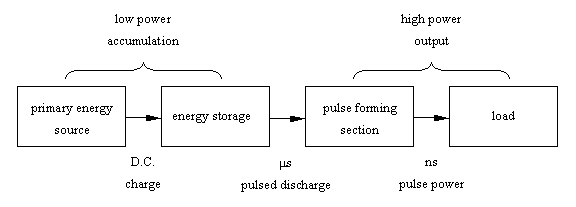
\includegraphics[height=4cm,width=8cm,keepaspectratio=true]{HPMsystem}
 \caption{Primjer ubacivanja slike.}
 \label{fig:prva}
	\end{center}
\end{figure}
\end{verbatim}
Uo�ite uporabu naredbe \verb|\label| unutar bloka. Na nju se potom u tekstu mo�emo referencirati pisanjem npr.\ \verb|Na Slici~\ref{fig:prva}| �ime \LaTeX{} u tekst uvrsti pripadaju�i broj slike, kao npr.\ ``Na Slici~\ref{fig:prva} prikazana je osnovna shema HPM sustava.''
Znak \verb|~| iza rije�i Slici osigurava to�no jedan znak razmaka, �to poma�e ukoliko je rije� Slika na kraju retka, da ne razdvoji rije� Slika i pripadaju�i broj slike.

\begin{figure}[!htbp]
	\begin{center}
 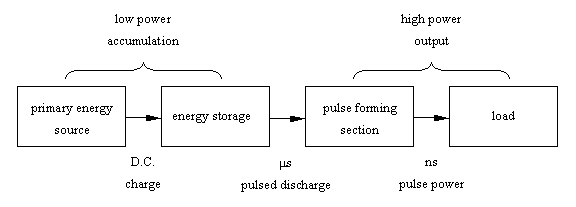
\includegraphics[height=4cm,width=8cm,keepaspectratio=true]{HPMsystem}
 \caption{Primjer ubacivanja slike.}
 \label{fig:prva}
	\end{center}
\end{figure}

Uo�ite i na�in prilago�avanja veli�ine slike. Parametri slike \emph{width} i \emph{height} odre�uju maksimalne dopu�tene dimenzije pri �emu se primarno po�tuje manju navedenu dimenziju, a \emph{keepaspectratio} osigurava zadr�avanje odnosa dimenzija slike, odnosno sprje�ava deformaciju slike, nakon proizvoljno unesenih veli�ina.

Uo�ite da sve oznake tj.\ \emph{labeli} ne smiju imati razmak u imenu. To vrijedi i op�enito, a ne samo za slike.

Tako�er, uo�ite da nije potrebno pisati ekstenziju slike jer to je ure�eno u postavkama glavnoga dokumenta pa time �tedi trud. Ekstenzije koje se mo�e izostaviti su: \emph{jpg}, \emph{jpeg}, \emph{png} i \emph{pdf}.

Shema prikazana na Slici~\ref{fig:prva} �e biti kori�tena i za potrebe idu�ih primjera, a {\color{blue} u mapi na va�em disku ju obri�ite nakon �to po�nete pohranjivati vlastite slike vezane uz va� rad}.


\section{Ubacivanje podslika}
Ponekada se jedna slika sastoji od dvije ili vi�e podslika kojima �elimo opisati neku cjelinu. Slika �e dobiti pripadni broj, a podslike slova (a), (b) itd.
To se mo�e posti�i sljede�om strukturom:
\begin{verbatim}
\begin{figure}[!htpb]
 \begin{center}
  \subfloat[Blok shema HPM sustava.]{\label{fig:HPM}
   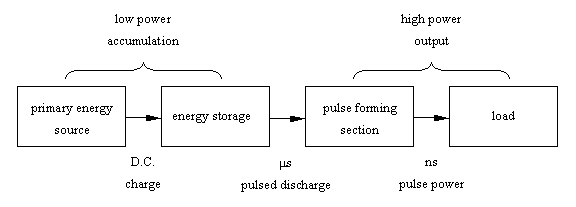
\includegraphics[height=5cm,width=10cm,keepaspectratio=true]{HPMsystem}}\\ 
	    %\hspace{10pt}
   \subfloat[JabRef su�elje za unos ``elektroni�ke'' reference.]
   {\label{fig:jabref}
   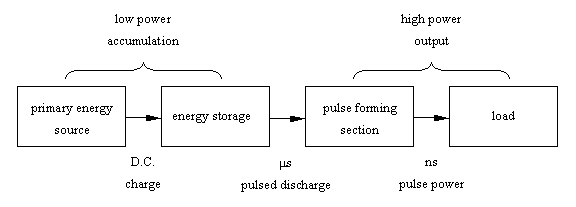
\includegraphics[height=7cm,keepaspectratio=true]{HPMsystem}}
\caption{Primjer ubacivanja vi�e podslika. Ovo je opis cijele slike.}
\label{fig:dvije_podslike}
  \end{center}
\end{figure}
\end{verbatim}
�to �e uvrstiti ono �to se vidi na Slici~\ref{fig:dvije_podslike}, koja se sastoji od dviju podslika.
Podslika~\ref{fig:HPM} pokazuje shemu HPM sustava, a podslika~\ref{fig:jabref} su�elje JabRef programa za unos bibliografskih jedinica.

\begin{figure}[!htpb]
	  \begin{center}
	   \subfloat[Blok shema HPM sustava.]{\label{fig:HPM} 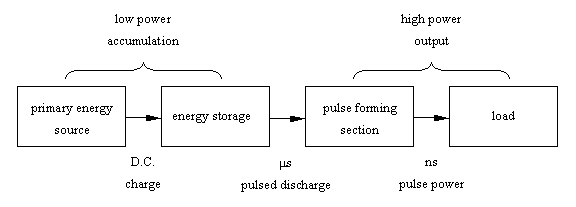
\includegraphics[height=5cm,width=10cm,keepaspectratio=true]{HPMsystem}} \\ %\hspace{10pt}
	   \subfloat[JabRef su�elje za unos ``elektroni�ke'' reference.]{\label{fig:jabref} 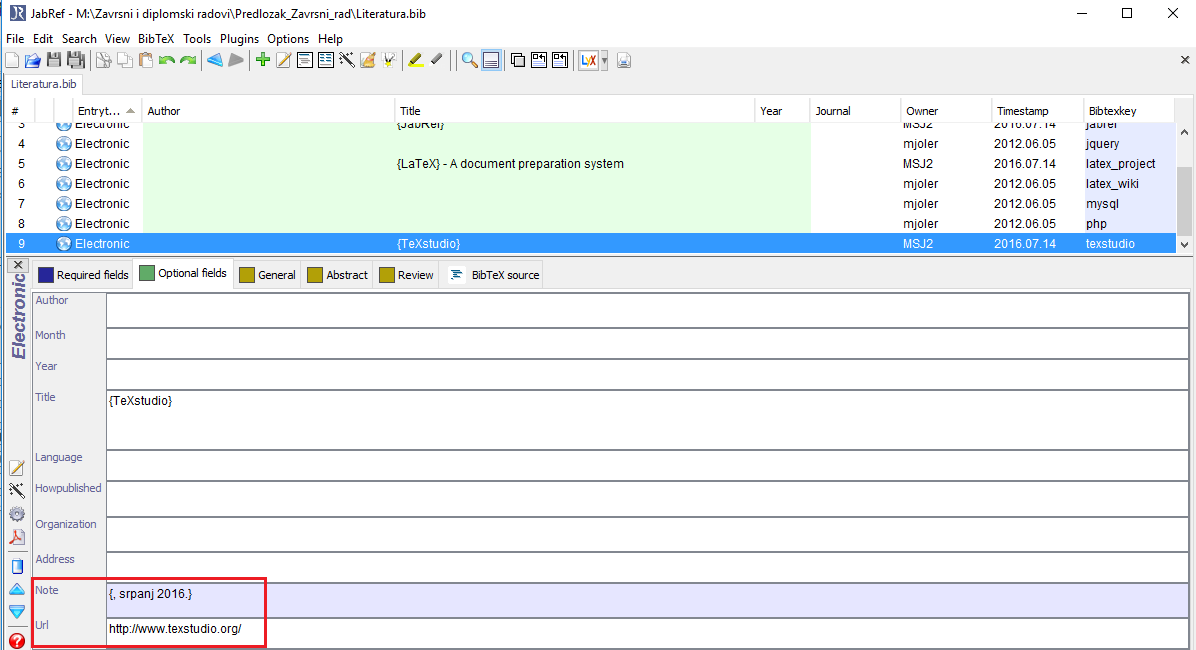
\includegraphics[height=7cm,keepaspectratio=true]{jabref}}
\caption{Primjer ubacivanja vi�e podslika. Ovo je opis cijele slike.}
\label{fig:dvije_podslike}
	  \end{center}
\end{figure}



\section{Ubacivanje tabele} 
Vi�e detalja o kreiranju tabela pro�itajte u literaturi, a sljede�i blok vam omogu�ava kreiranje jednostavne tabele, kao �to je prikazano u Tabeli~\ref{tab:prva}.
\begin{verbatim}
\begin{table}[!htbp]
\renewcommand{\arraystretch}{1.2}
\caption{Ovo je primjer izrade tabele.}
\centering
\begin{tabular}{|c|c|c|}
\hline
variabla & vrijednost 1 & vrijednost 2  \\ [0.5ex]
\hline \hline  
A & 5 & 3 \\ [0.5ex] % razmak do iducega retka
B & 4 & 2 \\ [0.5ex]
\hline
\end{tabular}
\label{tab:prva}
\end{table}
\end{verbatim}

\begin{table}[!htbp]
\renewcommand{\arraystretch}{1.2}
\caption{Ovo je primjer izrade tabele.}
\centering
\begin{tabular}{|c|c|c|}
\hline
variabla & vrijednost 1 & vrijednost 2  \\ [0.5ex]
\hline \hline 
A & 5 & 3 \\ [0.5ex] % razmak do iducega retka
B & 4 & 2 \\ [0.5ex]
\hline
\end{tabular}
\label{tab:prva}
\end{table}
%
Podaci koji su u stupcima se u tabeli razdvajaju znakom \&. Novi redak se na kraju aktualnoga retka formira znakom \verb|\\|. Broj stupaca se definira iza \emph{tabular} time �to se navedu slova koja ozna�avaju poravnavanje teksta u svakom stupcu, a broj slova zna�i broj stupaca koji �e biti kreiran u tabeli. Vertikalni razmak izme�u redaka u tabeli mo�ete za cijelu tabelu prilagoditi uporabom sljede�e sintakse prije strukture za tabelu:\\
\verb| \renewcommand{\arraystretch}{1.2} | gdje broj u zagradi na kraju (ovdje je 1.2) prilagodite sukladno va�oj preferenciji. Mo�e se prilagoditi i razmak za svaki pojedini redak (uo�ite \verb|[0.5ex]| na kraju redaka), ali to je manje od interesa jer tipi�no �elimo da svi retci imaju jednaki razmak jedni od drugih.

Sli�no mo�ete u�initi i za razmak izme�u stupaca tabele navo�enjem sljede�e sintakse prije bloka tabele:\\
\verb| \renewcommand{\tabcolsep}{0.3cm} |.



\section{Uporaba kratica u tekstu. Automatsko generiranje popisa kratica.}  \label{sec:kratice}
Listu kratica definirajte u datoteci \verb|Kratice.tex| (vidjeti predlo�ak unutar datoteke). U redovitom tekstu, kraticu  mo�ete ubaciti kori�tenjem naredbe \verb|\gls{ID_kratice}| gdje je \verb|ID_kraticE| identifikator kratice kako je definiran u datoteci \emph{Kratice.tex}. Pri prvoj uporabi naredbe \verb|\gls|, ispisat �e se najprije puni naziv pojma pa u zagradi kratica, a kod svake sljede�e uporabe, ispisat �e se samo kratica. Na primjer, kada (nakon prethodnog deklariranja u datoteci \verb|Kratice.tex|) upotrijebite \verb|\gls{gsm}| prvi puta, u tekstu �e se ispisati \gls{gsm}, a kada upotrijebite \verb|\gls{gsm}| drugi puta i dalje, u tekstu �e se ispisati samo \gls{gsm} (usporedi s definicijom kratice u datoteci \verb|Kratice.tex|). 
 
{\color{red} Listu kratica generirate sljede�im postupkom:} \label{generiranje_liste_kratica}
\begin{enumerate}
	\item Pokrenite kompilaciju cijeloga teksta jedanputa (to �e generirati neke datoteke koje su potrebne za daljnju obradu, specifi�no one s ekstenzijama .ist i .glo).
	\item Otvorite \emph{Command Prompt} aplikaciju na va�em ra�unalu i postavite se u radnu mapu gdje su vam datoteke za diplomski rad. 
	\item Potom pokrenite \emph{makeindex} rutinu (ona �e tipi�no biti ve� prisutna na va�em ra�unalu) upisuju�i sljede�u sintaksu: \\
	\verb|makeindex   -s myDoc.ist  -o myDoc.gls   myDoc.glo| \\
	gdje naziv datoteke \emph{myDoc} treba zamijeniti nazivom va�e glavne .tex datoteke, (npr. \verb|JMBAG_Ime_Prezime.tex|).
	\item Pokrenite \LaTeX{} jo� jednom ili dva puta, ako treba, dok se u uvodu pdf dokumenta ne pojavi lista kratica (pod naslovom \emph{Pojmovnik}).	
\end{enumerate}

Mo�da isprva zvu�i slo�eno, ali zapravo nije (bar ne uz ovako precizne upute!). Svaki puta kada dodate nove definicije kratica, potrebno je ponoviti ovaj postupak da bi se a�urirale odgovaraju�e datoteke i uredno prikazala potpuna lista u pdf-u (a i izbjegle poruke o pogre�kama tijekom kompajliranja teksta). 

Nije te�ko nakon �to prvi puta pro�ete ovaj postupak i omogu�ava vam u tekstu biti dosljedan u uporabi odre�ene kratice. Da izbjegnete �u�enje, va�no je jo� re�i da �e se ovim postupkom automatski stvoriti tek lista kratica koje ste u tekstu upotrijebili uporabom sintakse \verb|\gls|, a ne na temelju liste definicija koje ste naveli u datoteci \verb|Kratice.tex|. Zato, ako nijednom u tekstu ne upotrijebite sintaksu \verb|\gls|, ne�e biti ispisan ni popis kratica tj.\ \emph{Pojmovnik}. {\color{blue} Kako \LaTeX{} na kraju uvijek nagradi trud koji je ulo�en u savladavanje njegove sintakse, pogodnost ovakvoga automatskoga kreiranja Pojmovnika je i to �to uz svaki kraticu \LaTeX{} automatski ispi�e i brojeve stranica na kojima se doti�na kratica pojavljuje!} U elektroni�kom pdf dokumentu, brojevi stranica su ujedno i hiper-veze na te stranice pa se tako mo�e odmah sko�iti na stranicu gdje je pojedina kratica upotrijebljena.

Ukoliko vam se prethodno opisani postupak �ini preslo�enim, popis kratica mo�ete napraviti i ru�no, isto pomo�u datoteke Kratice.tex, u kojoj tako�er postoji kratki predlo�ak i za takav pristup. Za to je onda u osnovnoj datoteci \verb|JMBAG_Ima_Prezime.tex| potrebno deaktivirati liniju koda koja po�inje sa \verb|\printglossary|, a aktivirati blok koji po�inje sa \verb|\begin{glossary}| i zavr�ava sa \verb|end{glossary}|.



\section{Nagla�avanje teksta}
\subsection{Navodnici}
Za navodnike s lijeve strane fraze (otvaranje navodnika) koristi se 2x jednostruki navodnik koji se na tipkovnici nalazi lijevo od broja 1, a za navodnike s desne strane fraze (zatvaranje navodnika), koristi se 2x jednostruki navodnik koji se na tipkovnici nalazi na tipki \emph{�}, �to proizvede npr.\ ``abc''.

{\color{blue} Alternativno, u ovom paketu je pripremljena i naredba {\color{red} \verb|\navod{abc}|} gdje je \emph{abc} tekst koji se stavlja izme�u navodnika, tj.\ \navod{abc}.}

\subsection{Kosa i podebljana slova}
Nagla�avanje neke rije�i ili fraze pomo�u kosih (italic) slova mo�emo dobiti uporabom naredbe {\color{red} \verb|\emph{abc}|} ili pomo�u  {\color{red}\verb|\textit{abc}|} gdje je \emph{abc} neki tekst koji se �eli naglasiti.

\textbf{Podebljana slova} mo�emo posti�i uporabom naredbe {\color{red} \verb|\textbf{abc}|} gdje je \textit{abc} neki tekst koji �elimo podebljati.

\section{Verbatim: okru�enje za doslovni tekst}
Verbatim okru�enje omogu�ava ispis teksta u izvornom obliku, bez da ga \LaTeX{} tuma�i po svojiim sintakti�kim pravilima. To je pogodno kada se na stranicu  npr.\ �eli kopirati dio programskoga koda iz nekog jezika i kada �elimo zadr�ati sve izvorne znakove u nekoj frazi, bez da \LaTeX{} po�ne javljati pogre�ke kod kompajliranja, �to bi se moglo pojaviti kada se ne bi koristilo \emph{verbatim okru�enje}, po�to bi neke znakove interpretirao kao pogre�ke u sintaksi.

Postoji kra�i i du�i oblik verbatima. Kra�i slu�i za kra�u frazu od jedne ili par rije�i, a du�i za vi�e redaka.

\noindent Kra�i oblik verbatima ima sintaksu: \verb+\verb|neka fraza|+

\noindent Du�i oblik verbatima ima sintaksu:\\
\verb|\begin{verbatim}| \\
\verb|neki tekst| \\
\verb|\end{verbatim}| \\


\section{Kreiranje jedne jednad�be ili serije jednad�ba}

\subsection{Kreiranje jedne jednad�be}
Jednad�ba se napi�e u posebnom matemati�kom modu koji se kreira pomo�u bloka:
\begin{verbatim}
	\begin{equation}
		 A = B + C   \label{eq:prva}
	\end{equation}
\end{verbatim}
�to �e dati sljede�i izgled:
\begin{equation}
	 A = B + C   \label{eq:prva}
\end{equation}
Da bi se na nju referenciralo, na �eljenom mjestu u tekstu upi�emo \verb|\eqref{eq:prva}|, �ime �e se uvrstiti njezin pripadni (automatski generirani) broj, a za potpuniji smisao mo�emo npr.\ napisati \verb| Jednad�ba~\eqref{eq:prva}|, rezultat �ega je da �e u tekstu pisati Jednad�ba~\eqref{eq:prva}. 
Ako ju se ne �eli numerirati, onda se nakon rije�i \emph{begin} stavi zvjezdica, tj.\ \verb|begin*{equation}|.

\subsection{Kreiranje grupe jednad�ba}
Grupa jednad�ba se kreira uporabom \emph{subequations} sintakse. Na primjer, sljede�i blok �e definirati dvije podjednad�be u grupi, gdje �e svaka biti numerirana istim brojem, a razlikovati slovom iza broja.
\begin{verbatim}
	\begin{subequations}
		\begin{align}
		        A &= B + C  	\label{subeq:prva} \\
		        D &= F + G		\label{subeq:druga}
		\end{align}
	\label{subeq:obje}
	\end{subequations}
\end{verbatim}

To �e u izlaznom dokumentu rezultirati sljede�im izgledom:
\begin{subequations}
\begin{align}
        A &= B + C  	\label{subeq:prva} \\
        D &= F + G		\label{subeq:druga}
\end{align}
\label{subeq:obje}
\end{subequations}
U \eqref{subeq:prva} je prikazano dobivanje vrijednosti $A$, a u \eqref{subeq:druga} je prikazano dobivanje vrijednosti $D$. Jednad�ba~\eqref{subeq:obje} je \emph{�uveni studentov zakon}!



\section{Liste}
Liste su �este forme u tekstu kojima se na pregledni na�in nabrajaju neke stavke. Stavke obi�no navodimo ili s to�kama na po�etku, s brojevima ili sa slovima. U \LaTeX-u su upravo ta tri stila unaprijed definirana, a mogu�e su i slo�enije definicije stilova i kombinacije lista.

\subsection{Lista s to�kama}
Lista s to�kama se postigne blokom
\begin{verbatim}
\begin{itemize}
    \item prva nenumerirana stavka
    \item druga nenumerirana stavka
\end{itemize}
\end{verbatim}
�to na ekranu proizvede:
\begin{itemize}
% \setlength\itemsep{1ex}   % za lokalnu prilagodbu
	\item prva nenumerirana stavka
	\item druga nenumerirana stavka
\end{itemize}

\subsection{Lista s brojevima}
Numerirana lista s brojevima se postigne blokom
\begin{verbatim}
\begin{enumerate}[itemsep=1ex, topsep=4pt, partopsep=0pt]
     \item prva numerirana stavka
     \item druga numerirana stavka
\end{enumerate}
\end{verbatim}
U uglatoj zagradi su tri parametra kojima se to�no mo�e kontrolirati vertikalni razmak izme�u stavki u listi (\emph{itemsep}), razmak izme�u prethodnoga teksta i prve stavke u listi (\emph{topsep}) i dodatni prostor izme�u liste i prethodnoga paragrafa kada lista zapo�inje novi paragraf (\emph{partopsep}), ali te parametre \textbf{ne morate navoditi} tj.\ tu uglatu zagradu ne morate pisati. Tada �e se primijeniti vrijednosti parametara koje su definirane za cijeli dokument, a ove parametre se mo�e upotrijebiti tek da u nekom pojedinom slu�aju prilagodite razmake.
Za osjetiti efekte ovih parametara, najbolje se malo sam poigrati razli�itim vrijednostima parametara i vidjeti posljedice toga na listu (pri tome se uz brojeve kao prikladne jedinice za razmak mogu koristiti \emph{pt}, \emph{ex} ili \emph{em}).

\subsection{Proizvoljno ozna�ena lista}
Takva se lista mo�e posti�i u sklopu op�enitije forme koja omogu�uje proizvoljni opis ispred pojedine stavke, pomo�u sljede�ega bloka:
\begin{verbatim}
\begin{description}
     \item[a)] prva opisna stavka
     \item[b)] druga opisna stavka
\end{description}
\end{verbatim}
�to na ekranu proizvede:
\begin{description}%[itemsep=1ex, topsep=4pt, partopsep=0pt] za lokalnu prilagodbu
	\item[a)] prva opisna stavka
	\item[b)] druga opisna stavka \\
\end{description}
%
Kod ove strukture, u uglatu zagradu iza naredbe \verb|\item|, navodi se proizvoljna oznaka kojom se �eli na neki na�in ``numerirati'' listu.
%:::::::::::::::::::::::::::::::::::::::::::::::::::
\chapter{Dodatne informacije}
\section{Primjeri uporabe sintakti�kih struktura}
\begin{enumerate}
	\item Za uvid u kontekstualnu primjenu raznih sintakti�kih struktura, mo�ete otvoriti datoteku \href{run:Intro.tex}{{\color{blue}Intro.tex}}, unutar koje su napisane i ove upute. 
	\item Primjere slo�enijih sintakti�kih struktura, kao �to su ubacivanje slike, tabele ili jednad�be, mo�ete na�i u datoteci \href{run:sintaksa_cestih_struktura.tex}{{\color{blue}sintaksa\_cestih\_struktura.tex}} koja je dio paketa. Odabrane se strukture mo�e kopirati i zalijepiti u va� tekst, uz minimalne prilagodbe kao �to su naziv slike, veli�ina slike, opis i ID slike, a analogno i za tabele i jednad�be.
	\item Kona�no, za vi�e detalja o bilo �emu, potra�ite informacije u dvama priru�nicima koji su prilo�eni u mapi \href{run:prirucnici}{{\color{blue}prirucnici}} ili na webu, gdje se, me�u obiljem drugih informacija, nalaze i korisne wiki stranice \cite{latex_wiki,tex_exchange} o \LaTeX-u pomo�u kojih se obi�no brzo prona�e upute i zadovoljavaju�e rje�enje kakvom sintaksom se mo�e urediti �eljeni dio teksta.
\end{enumerate}

\section{Savjeti za lak�e ure�ivanje teksta}
Vjerujem da vam ovaj dokument mo�e uvelike pomo�i u pripremi teksta va�ega zavr�nog/diplomskog rada i omogu�iti da glavninu vremena tro�ite na sadr�aj rada, a manje na formatiranje rada jer to �e za vas sada obaviti \LaTeX{}! 

No, korektnosti radi, potrebno je napomenuti i sljede�e: \LaTeX{} je vrlo osjetljiv na pogre�ke u sintaksi naredbi (da, ba� kao �to su i programski jezici) pa vas mo�e povremeno ugnjaviti javljanjem pogre�ke koju nikako ne uspijevate uo�iti gdje je. Iskustvo kojim se izbjegava ta nelagoda jest sljede�e:
\begin{itemize}
	\item svako poglavlje napi�ite u novoj datoteci (da biste koli�inu teksta razdvojili na preglednije i manje cjeline) koju imenujte prikladnim imenom (bez razmaka u imenu). Potom te datoteke samo pozivajte iz glavnoga dokumenta \verb|JMBAG_Ime_Prezime.tex| pomo�u naredbe \verb|\include{ime_datoteke}|. Takav je pristup upravo i kori�ten u pripremi ovoga paketa.
	%
	\item {\color{red} budite koncentrirani dok pi�ete \LaTeX{} naredbe, poglavito zagrade, posebne znakove i matemati�ki tekst gdje se zahtijeva uporaba znaka \$!}
	%
	\item kompajlirajte tekst prije nego se skupi puno teksta jer tako �ete imati manje teksta za prekontrolirati u slu�aju pogre�ke. Tako�er vam za provjeru tek manjega dijela dokumenta mo�e pomo�i paket \verb|\usepackage{syntonly}| i naredba \verb|syntaxonly|, a isto tako i naredba \verb|\includeonly{ime_datoteke}| kojom �ete kompajlirati samo tu navedenu datoteku, �ime  ispred ``ne�eljenih'' datoteka ne morate stavljati znak ``komentara'' (\%).
	%
	\item ako niste sigurni ho�e li vam raditi neka naredba nakon pisanja, radije tekst kompajlirajte odmah po pisanju te naredbe---da vidite �to �ete dobiti i rije�ite dvojbu, nego da �ekate da se skupi jo� dubioznih mjesta u tekstu, kada �e nakon kompajliranja biti te�e detektirati koja linija teksta zapravo izaziva probleme (\LaTeX-ov prozor s porukama �esto nije odve� precizan u lociranju i opisu pogre�aka, ovisno o editoru teksta koji koristite).
\end{itemize}


\section{Zavr�ne napomene}
Ovime zaklju�ujemo uvodne upute koje �e najve�em broju studenata biti dovoljne (ili barem dovoljna osnova) za uspje�no pisanje zavr�nog odnosno diplomskog rada.

Prije nego prije�ete na kreiranje vlastitoga sadr�aja u�inite jo� sljede�e akcije kojima �ete deaktivirati dio paketa koji �e biti nepotreban:
\begin{enumerate}
	\item u mapi \href{run:slike}{{\color{blue}slike}}, obri�ite datoteke \verb|HPMsystem.png| i \verb|jabref.png| jer su one slu�ile tek za ilustracije u ovim Uputama.
	%
	\item u glavnoj datoteci  \href{run:JMBAG\_Ime\_Prezime.tex}{{\color{blue}JMBAG\_Ime\_Prezime.tex}} stavite znak komentara ``\%'' ispred linije \verb|\include{Intro}| kojom se pozivaju ove upute ili obri�ite tu liniju koda, �ime to vi�e ne�e biti uklju�eno u tekst va�eg vlastitoga rada.
\end{enumerate}

Budite slobodni emailati svoje dojmove o razumljivosti i prakti�nosti ovoga materijala, kao i informacije o uo�enim pogre�kama u tekstu. \\

\noindent Ugodan rad! \\

\noindent Miroslav Joler	\\	
\href{mailto:mjoler@riteh.hr}{mjoler@riteh.hr}	\\ \\


{\color{red} A sada, prije�ite na kreiranje vlastitoga sadr�aja, pri �emu �e vam, za po�etak, pomo�i vodi� iz sljede�ega poglavlja.}


\chapter{Vodi� za pisanje vlastitoga teksta}

\section{Upis uvodnih podataka}
\begin{enumerate}
	\item {\color{red} \textbf{Otvaranje glavne datoteke.}} Pokrenite va� editor \LaTeX{} teksta i iz njega otvorite sredi�nju datoteku ovoga predlo�ka za pisanje rada, koja je nazvana \href{run:JMBAG\_Ime\_Prezime.tex}{{\color{blue}JMBAG\_Ime\_Prezime.tex}} i nalazi se u sredi�njoj mapi unutar ovoga paketa (ili probajte klikom na prethodnu poveznicu u tekstu).
	%
	\item {\color{red} \textbf{Upis uvodnih podataka.}} U gornjem dijelu dokumenta nemate ni�ta za mijenjati, nego skrolajte prema dolje do linije koja glasi: \verb|\begin{document}|. Specifi�ni podaci koje student/ica nakon toga treba upisati bit �e uz sljede�e naredbe:
	\begin{itemize}
		\item \verb|\degreesubject|: upisati razinu studija koji poha�ate (npr.\ Preddiplomski studij ra�unarstva ili Diplomski studij ra�unarstva i sl.)
		\item \verb|\documenttype|: upisati \emph{Zavr�ni rad} ili \emph{Diplomski rad}
		\item \verb|\title|: upisati naslov rada kako je zadano u slu�benom zadatku
%\item \verb|\date|: upisati samo mjesec predaje rada. Godina se upisuje automatski.
		\item \verb|\author|: upisati svoje ime i prezime
		\item \verb|\jmbag|: zamijeniti postoje�i broj vlastitim JMBAG brojem 
		\item \verb|\mentor|: upisati titulu te ime i prezime svojega mentora
	\end{itemize}
	%
	\item {\color{red} \textbf{Prva kompilacija teksta.}} \label{encoding2} \textbf{POZOR: prije prve kompilacije teksta, uvjerite se da vam je kodna stranica postavljena na ``windows-1250'' (alternativni naziv: ``cp1250''). Ona je kod kompilacije klju�na za ispravno ispisivanje hrvatskih dijakriti�kih znakova u izlaznom PDF dokumentu! Vidite stranicu~\pageref{encoding1} za dodatne upute o postavljanju te kodne stranice.} 
	
	Za prvu probu nakon une�enih podataka, kompajlirajte dokument na na�in da unutar va�ega \emph{TeXstudio} editora odaberete opciju izbornika \emph{Tools} koja je nazvana \emph{Build \& View} ili, kra�e, samo stisnete tipku F5 ili kliknete na ikonu dvostrukog zelenog trokuta u glavnoj traci alata. To pokrene postupak kompajliranja svega i rezultat bi trebao biti \emph{PDF} datoteka u kojoj �ete vidjeti lijepo formatirane po�etne stranice rada. \\
	Za prvu kompilaciju budite strpljivi jer \LaTeX{} �e mo�da tijekom postupka kompilacije povla�iti neke vanjske pakete koji mu trebaju, a nisu jo� prisutni na va�em ra�unalu nakon instalacije \LaTeX-a. U takvom slu�aju, tipi�no se dovoljno strpjeti oko 30~s prije nego se pojavi PDF dokument kao rezultat kompilacije. Ukoliko se to ne dogodi, u prozoru s porukama �e vam \LaTeX{} mo�ebitno napisati da mu nedostaje neka datoteka sa .sty ekstenzijom, �to zna�i da automatsko povla�enje ili nije namje�teno kao opcija u va�oj \LaTeX{} instalaciji (ali mo�e se namjestiti u postavkama \LaTeX-a) ili nije uspjelo pa tra�eni paket mo�ete sami na webu potra�iti i povu�i na va�e ra�unalo (najjednostavnije je uvrstiti ga u glavnu mapu va�ega projekta). Pozor: 
		\begin{itemize}
			\item TeXstudio u startu ve� ima postavljen \emph{PDF} kao format izlaznoga dokumenta, ali ukoliko to iz nekog razloga ne bude slu�aj, mo�e se postaviti u izborniku i opcijama za konfiguraciju TeXstudia. 
			%
			\item ponekada je potrebno 2-3 puta pokrenuti \emph{Build} operaciju da bi sve promjene bile a�urirane u \emph{PDF} dokumentu kao �to su npr.\ brojevi referenca, popis literature i sl. (TeXstudio, po potrebi, �esto sam automatski pokrene kompajliranje dva puta zaredom, ali po�to to ne mora biti slu�aj svaki puta, dobro je za znati pa onda vi ru�no pokrenete drugi puta.)
		\end{itemize}
	%
	\item {\color{red} \textbf{Promjena naziva glavne datoteke.}} Zatvorite \verb|JMBAG_Ime_Prezime.tex| datoteku (i svaku drugu ako je jo� neka \emph{tex} datoteka otvorena) i u mapi {\color{red} promijenite ime \verb|JMBAG_Ime_Prezime.tex| datoteke} na na�in da {\color{red} JMBAG, ime i prezime zamijenite va�im specifi�nim podacima}. Potom ponovo otvorite tu datoteku jer ona je sredi�nja datoteka koja slu�i za kompajliranje cijeloga projekta i mora biti otvorena uvijek kada se kompajlira tekst (drugim rije�ima, tu datoteku kompajlirate). \textbf{(Nakon �to idu�i put kompjalirate projekt pod novim imenom, obri�ite u va�oj radnoj mapi sve datoteke koje nose staro ime!)}
	%
	\item {\color{red} \textbf{Definiranje \emph{Posvete}.}} (Neobavezno). Ako �elite napisati kratku posvetu (pazi, posveta nije isto �to i zahvala, koju imate priliku definirati nakon toga) nekome (majci, ocu, roditeljima i sl.), u glavnoj datoteci va�ega rada (stari naziv \verb|JMBAG_Ime_Prezime.tex| koji ste zamijenili novim nazivom) prona�ite blok koji po�inje tekstom \verb|\begin{dedication}| i u liniji ispod toga tekst predlo�ka zamijenite nekim va�im tekstom suvisle posvete. \\
	Ukoliko nemate potrebu upisati neku Posvetu, u tom slu�aju (o)stavite znakove komentara \verb|%| ispred te tri linije koda, da biste to deaktivirali kod kompilacije teksta.
	%
	\item {\color{red} \textbf{Definiranje \emph{Zahvale}.}} (Neobavezno). Ako �elite napisati zahvalu nekome (npr.\ mentoru za savjete, roditeljima ili bliskoj osobi za potporu tijekom studija, kolegama za pomo� pri radu i sl.), otvorite datoteku \href{run:Zahvala.tex}{{\color{blue}Zahvala.tex}} i zamijenite tekst predlo�ka nekim va�im osobnim tekstom. Ostale linije predlo�ka ne mijenjajte. Potom snimite datoteku (Ctrl+S) i zatvorite.\\ 
	Ukoliko nemate potrebu pisati neku zahvalu, prona�ite u glavnoj datoteci blok koji po�inje tekstom \verb|\begin{acknowledgments}| i sve linije toga bloka stavite u komentar. \\
	Naknadne izmjene i prilagodbe teksta Zahvale mo�ete u�initi izmjenama u datoteci \verb|Zahvala.tex|, a aktiviranje ili deaktiviranje teksta Zahvale uklanjanjem ili postavljanjem komentara na taj blok koda u glavnoj datoteci.
	%
	\item {\color{red} \textbf{Ure�enje \emph{Izjave o samostalnoj izradi rada}.}} (Obavezno). Otvorite datoteku \href{run:Izjava.tex}{{\color{blue}Izjava.tex}} i:
	\begin{enumerate}
		\item po �elji, prilagodite tekst izjave s obzirom na rod glagola (``izradio'' ili ``izradila'')
		\item  u retku gdje pi�e \verb|Ime Prezime|, umjesto toga upi�ite svoje ime i prezime.
		\item pomo�u linije \verb+\verb|  |+ regulirajte poravnanje imena i prezimena s gornjom crtom.
	\end{enumerate}
	Snimite datoteku na disk i zatvorite.
\end{enumerate}

\section{Po�etak pisanja glavnoga dijela rada}
\begin{enumerate}
	\item {\color{red} \textbf{Pisanje prvoga poglavlja.}} Otvorite datoteku  \href{run:Poglavlje\_1.tex}{{\color{blue}Poglavlje\_1.tex}} i po�nite pisati svoj vlastiti tekst uz postavljanje naslova poglavlja i sekcija (tj. potpoglavlja) po vlastitom izboru, a na kraju proizvoljno mo�ete promijeniti ime te datoteke u ne�to �to odgovara sadr�aju va�ega poglavlja i to ime stavite u \verb|\include| naredbu umjesto inicijalnoga naziva \verb|Poglavlje_1| (ako vas ne smeta, mo�ete i ostaviti naziv \verb|Poglavlje_1|).\\ Da bi se tekst toga \verb|Poglavlja_1| uspje�no kompajlirao u izlazni dokument, uklonite znak komentara ``\%'' ispred \verb|\include{Poglavlje_1}| naredbe u glavnoj datoteci (stari naziv datoteke bio je  \href{run:JMBAG\_Ime\_Prezime.tex}{{\color{blue}JMBAG\_Ime\_Prezime.tex}}). Tako u�inite i za sva nova poglavlja koja �ete potom kreirati.
	%
	\item {\color{red} \textbf{Definiranje \emph{Literature.}}} Popis literature se gradi sukcesivno tijekom pisanja rada. Kao �to je opisano u Sekciji~\ref{sec:RefLit} na stranici \pageref{sec:RefLit}, popis literature mo�ete graditi na dva na�ina---sa i bez uporabe JabRef programa, a oba na�ina su omogu�ena u datoteci \href{run:Literatura.tex}{{\color{blue}Literatura.tex}}.\\ 
	Za onaj na�in za koji ste se odlu�ili, uklonite komentare ispred toga bloka naredbi u datoteci \verb|Literatura.tex|, a za onaj drugi na�in postavite znakove komentara, da biste taj drugi na�in onesposobili kod kompajliranja teksta.\\
	\emph{Spoznajte da se u popisu literature smiju na�i samo one stavke koje su referencirane u radu}! Drugim rije�ima, ne mo�ete definirati popis literature, a da se na pojedinu stavku nijednom ne referencirate u tekstu rada! S druge strane, na pojedinu se literaturu mo�ete u radu referencirati koliko god puta ho�ete, ali u popisu literature ju se navodi samo jedanput!
	
	{\color{red} POZOR: ponekada se dogodi da postupak kompajliranja teksta (tvrdoglavo) ne�e osvje�iti popis literature nakon �to je u njemu bilo izmjena (npr. redoslijed stavki, redni brojevi i sl.), �ak ni nakon dvaju pokretanja kompajlera. \textbf{Tada je najbolje obrisati pomo�ne datoteke (me�u kojima je i \emph{.bbl} datoteka koja je ``zadu�ena'' za popis literature) uporabom naredbe ``Clean Auxiliary Files\dots'', koja se nalazi pod izbornikom \emph{Tools}, pa ponovo pokrenuti kompajler dva puta.}} Brisanje pomo�nih datoteka ima efekt ``�istoga starta'' i uglavnom �e dati �eljeni rezultat, a kada ni to ne bi pomoglo, onda se mo�e ru�nim intervencijama u datoteci \emph{.bbl} izvr�iti potrebne promjene.
	%
	\item {\color{red} \textbf{Definiranje \emph{kratica}}} za pojmove kori�tene u tekstu (neobavezno). Kratice i pripadaju�e pune nazive pojmova definirajte u datoteci \href{run:Kratice.tex}{{\color{blue}Kratice.tex}}, prema po�etnom predlo�ku koji je u njoj dan. Listu mo�ete sukcesivno pro�irivati svaki puta kada na�ete potrebu definirati neki novi pojam s kraticom.\\
	Uporaba kratica u tekstu je opisana u Sekciji~\ref{sec:kratice}, ali popis kratica (u tekstu zvan \emph{Pojmovnik}) ne�e automatski biti pro�iren novim kraticama, ve� za to trebate provesti postupak za \hyperref[generiranje_liste_kratica]{{\color{blue} generiranje liste kratica}} koji je opisan u Sekciji~\ref{sec:kratice}.
	%
	\item {\color{red} \textbf{Pisanje ostalih dijelova rada.}} Nastavite pisati rad definiranjem \emph{Poglavlja~2}, \emph{Poglavlja~3} itd.\, analogno kako ste �inili za \emph{Poglavlje~1}\dots
	%
	\item {\color{red} \textbf{Upis Sa�etka rada.}}\\
	Na kraju rada, a prije mo�ebitnih (neobaveznih) priloga, potrebno je napisati \emph{Sa�etak} rada i \emph{klju�ne rije�i} na hrvatskom i engleskom (gdje je to naslovljeno s \emph{Abstract} odnosno \emph{keywords}). \\
	Sa�etak je forma kratkoga teksta (1-3 paragrafa ukupne du�ine manje od pola stranice) u kojemu navedete \emph{�to} je u radu prikazano i \emph{ne ulazite u daljnja obja�njavanja}.\\
	Za upis \emph{Sa�etka} i \emph{klju�nih rije�i} odnosno \emph{Abstract}-a i \emph{keywords}-a, otvorite datoteku \href{Sazetak.tex}{{\color{blue}Sazetak.tex}} i tekst predlo�ka zamijenite vlastitim tekstom sa�etaka i klju�nih rije�i na hrvatskom i engleskom, a ostatak strukture koda nemojte mijenjati.
\end{enumerate}

\vspace{10pt}

\begin{flushright}
	Sretno! \\
	Miroslav Joler \\
	\href{mailto:mjoler@riteh.hr}{mjoler@riteh.hr}
\end{flushright}

| kojom se pozivaju ove upute ili obri�ite tu liniju koda, �ime to vi�e ne�e biti uklju�eno u tekst va�eg vlastitoga rada.
\end{enumerate}

Budite slobodni emailati svoje dojmove o razumljivosti i prakti�nosti ovoga materijala, kao i informacije o uo�enim pogre�kama u tekstu. \\

\noindent Ugodan rad! \\

\noindent Miroslav Joler	\\	
\href{mailto:mjoler@riteh.hr}{mjoler@riteh.hr}	\\ \\


{\color{red} A sada, prije�ite na kreiranje vlastitoga sadr�aja, pri �emu �e vam, za po�etak, pomo�i vodi� iz sljede�ega poglavlja.}


\chapter{Vodi� za pisanje vlastitoga teksta}

\section{Upis uvodnih podataka}
\begin{enumerate}
	\item {\color{red} \textbf{Otvaranje glavne datoteke.}} Pokrenite va� editor \LaTeX{} teksta i iz njega otvorite sredi�nju datoteku ovoga predlo�ka za pisanje rada, koja je nazvana \href{run:JMBAG\_Ime\_Prezime.tex}{{\color{blue}JMBAG\_Ime\_Prezime.tex}} i nalazi se u sredi�njoj mapi unutar ovoga paketa (ili probajte klikom na prethodnu poveznicu u tekstu).
	%
	\item {\color{red} \textbf{Upis uvodnih podataka.}} U gornjem dijelu dokumenta nemate ni�ta za mijenjati, nego skrolajte prema dolje do linije koja glasi: \verb|\begin{document}|. Specifi�ni podaci koje student/ica nakon toga treba upisati bit �e uz sljede�e naredbe:
	\begin{itemize}
		\item \verb|\degreesubject|: upisati razinu studija koji poha�ate (npr.\ Preddiplomski studij ra�unarstva ili Diplomski studij ra�unarstva i sl.)
		\item \verb|\documenttype|: upisati \emph{Zavr�ni rad} ili \emph{Diplomski rad}
		\item \verb|\title|: upisati naslov rada kako je zadano u slu�benom zadatku
%\item \verb|\date|: upisati samo mjesec predaje rada. Godina se upisuje automatski.
		\item \verb|\author|: upisati svoje ime i prezime
		\item \verb|\jmbag|: zamijeniti postoje�i broj vlastitim JMBAG brojem 
		\item \verb|\mentor|: upisati titulu te ime i prezime svojega mentora
	\end{itemize}
	%
	\item {\color{red} \textbf{Prva kompilacija teksta.}} \label{encoding2} \textbf{POZOR: prije prve kompilacije teksta, uvjerite se da vam je kodna stranica postavljena na ``windows-1250'' (alternativni naziv: ``cp1250''). Ona je kod kompilacije klju�na za ispravno ispisivanje hrvatskih dijakriti�kih znakova u izlaznom PDF dokumentu! Vidite stranicu~\pageref{encoding1} za dodatne upute o postavljanju te kodne stranice.} 
	
	Za prvu probu nakon une�enih podataka, kompajlirajte dokument na na�in da unutar va�ega \emph{TeXstudio} editora odaberete opciju izbornika \emph{Tools} koja je nazvana \emph{Build \& View} ili, kra�e, samo stisnete tipku F5 ili kliknete na ikonu dvostrukog zelenog trokuta u glavnoj traci alata. To pokrene postupak kompajliranja svega i rezultat bi trebao biti \emph{PDF} datoteka u kojoj �ete vidjeti lijepo formatirane po�etne stranice rada. \\
	Za prvu kompilaciju budite strpljivi jer \LaTeX{} �e mo�da tijekom postupka kompilacije povla�iti neke vanjske pakete koji mu trebaju, a nisu jo� prisutni na va�em ra�unalu nakon instalacije \LaTeX-a. U takvom slu�aju, tipi�no se dovoljno strpjeti oko 30~s prije nego se pojavi PDF dokument kao rezultat kompilacije. Ukoliko se to ne dogodi, u prozoru s porukama �e vam \LaTeX{} mo�ebitno napisati da mu nedostaje neka datoteka sa .sty ekstenzijom, �to zna�i da automatsko povla�enje ili nije namje�teno kao opcija u va�oj \LaTeX{} instalaciji (ali mo�e se namjestiti u postavkama \LaTeX-a) ili nije uspjelo pa tra�eni paket mo�ete sami na webu potra�iti i povu�i na va�e ra�unalo (najjednostavnije je uvrstiti ga u glavnu mapu va�ega projekta). Pozor: 
		\begin{itemize}
			\item TeXstudio u startu ve� ima postavljen \emph{PDF} kao format izlaznoga dokumenta, ali ukoliko to iz nekog razloga ne bude slu�aj, mo�e se postaviti u izborniku i opcijama za konfiguraciju TeXstudia. 
			%
			\item ponekada je potrebno 2-3 puta pokrenuti \emph{Build} operaciju da bi sve promjene bile a�urirane u \emph{PDF} dokumentu kao �to su npr.\ brojevi referenca, popis literature i sl. (TeXstudio, po potrebi, �esto sam automatski pokrene kompajliranje dva puta zaredom, ali po�to to ne mora biti slu�aj svaki puta, dobro je za znati pa onda vi ru�no pokrenete drugi puta.)
		\end{itemize}
	%
	\item {\color{red} \textbf{Promjena naziva glavne datoteke.}} Zatvorite \verb|JMBAG_Ime_Prezime.tex| datoteku (i svaku drugu ako je jo� neka \emph{tex} datoteka otvorena) i u mapi {\color{red} promijenite ime \verb|JMBAG_Ime_Prezime.tex| datoteke} na na�in da {\color{red} JMBAG, ime i prezime zamijenite va�im specifi�nim podacima}. Potom ponovo otvorite tu datoteku jer ona je sredi�nja datoteka koja slu�i za kompajliranje cijeloga projekta i mora biti otvorena uvijek kada se kompajlira tekst (drugim rije�ima, tu datoteku kompajlirate). \textbf{(Nakon �to idu�i put kompjalirate projekt pod novim imenom, obri�ite u va�oj radnoj mapi sve datoteke koje nose staro ime!)}
	%
	\item {\color{red} \textbf{Definiranje \emph{Posvete}.}} (Neobavezno). Ako �elite napisati kratku posvetu (pazi, posveta nije isto �to i zahvala, koju imate priliku definirati nakon toga) nekome (majci, ocu, roditeljima i sl.), u glavnoj datoteci va�ega rada (stari naziv \verb|JMBAG_Ime_Prezime.tex| koji ste zamijenili novim nazivom) prona�ite blok koji po�inje tekstom \verb|\begin{dedication}| i u liniji ispod toga tekst predlo�ka zamijenite nekim va�im tekstom suvisle posvete. \\
	Ukoliko nemate potrebu upisati neku Posvetu, u tom slu�aju (o)stavite znakove komentara \verb|%| ispred te tri linije koda, da biste to deaktivirali kod kompilacije teksta.
	%
	\item {\color{red} \textbf{Definiranje \emph{Zahvale}.}} (Neobavezno). Ako �elite napisati zahvalu nekome (npr.\ mentoru za savjete, roditeljima ili bliskoj osobi za potporu tijekom studija, kolegama za pomo� pri radu i sl.), otvorite datoteku \href{run:Zahvala.tex}{{\color{blue}Zahvala.tex}} i zamijenite tekst predlo�ka nekim va�im osobnim tekstom. Ostale linije predlo�ka ne mijenjajte. Potom snimite datoteku (Ctrl+S) i zatvorite.\\ 
	Ukoliko nemate potrebu pisati neku zahvalu, prona�ite u glavnoj datoteci blok koji po�inje tekstom \verb|\begin{acknowledgments}| i sve linije toga bloka stavite u komentar. \\
	Naknadne izmjene i prilagodbe teksta Zahvale mo�ete u�initi izmjenama u datoteci \verb|Zahvala.tex|, a aktiviranje ili deaktiviranje teksta Zahvale uklanjanjem ili postavljanjem komentara na taj blok koda u glavnoj datoteci.
	%
	\item {\color{red} \textbf{Ure�enje \emph{Izjave o samostalnoj izradi rada}.}} (Obavezno). Otvorite datoteku \href{run:Izjava.tex}{{\color{blue}Izjava.tex}} i:
	\begin{enumerate}
		\item po �elji, prilagodite tekst izjave s obzirom na rod glagola (``izradio'' ili ``izradila'')
		\item  u retku gdje pi�e \verb|Ime Prezime|, umjesto toga upi�ite svoje ime i prezime.
		\item pomo�u linije \verb+\verb|  |+ regulirajte poravnanje imena i prezimena s gornjom crtom.
	\end{enumerate}
	Snimite datoteku na disk i zatvorite.
\end{enumerate}

\section{Po�etak pisanja glavnoga dijela rada}
\begin{enumerate}
	\item {\color{red} \textbf{Pisanje prvoga poglavlja.}} Otvorite datoteku  \href{run:Poglavlje\_1.tex}{{\color{blue}Poglavlje\_1.tex}} i po�nite pisati svoj vlastiti tekst uz postavljanje naslova poglavlja i sekcija (tj. potpoglavlja) po vlastitom izboru, a na kraju proizvoljno mo�ete promijeniti ime te datoteke u ne�to �to odgovara sadr�aju va�ega poglavlja i to ime stavite u \verb|\include| naredbu umjesto inicijalnoga naziva \verb|Poglavlje_1| (ako vas ne smeta, mo�ete i ostaviti naziv \verb|Poglavlje_1|).\\ Da bi se tekst toga \verb|Poglavlja_1| uspje�no kompajlirao u izlazni dokument, uklonite znak komentara ``\%'' ispred \verb|\chapter{Naslov poglavlja}

\section{Naslov sekcije}

\section{Naslov sekcije}

% itd.

%%%%  POGLAVLJE ZAVRSENO  %%%%%
| naredbe u glavnoj datoteci (stari naziv datoteke bio je  \href{run:JMBAG\_Ime\_Prezime.tex}{{\color{blue}JMBAG\_Ime\_Prezime.tex}}). Tako u�inite i za sva nova poglavlja koja �ete potom kreirati.
	%
	\item {\color{red} \textbf{Definiranje \emph{Literature.}}} Popis literature se gradi sukcesivno tijekom pisanja rada. Kao �to je opisano u Sekciji~\ref{sec:RefLit} na stranici \pageref{sec:RefLit}, popis literature mo�ete graditi na dva na�ina---sa i bez uporabe JabRef programa, a oba na�ina su omogu�ena u datoteci \href{run:Literatura.tex}{{\color{blue}Literatura.tex}}.\\ 
	Za onaj na�in za koji ste se odlu�ili, uklonite komentare ispred toga bloka naredbi u datoteci \verb|Literatura.tex|, a za onaj drugi na�in postavite znakove komentara, da biste taj drugi na�in onesposobili kod kompajliranja teksta.\\
	\emph{Spoznajte da se u popisu literature smiju na�i samo one stavke koje su referencirane u radu}! Drugim rije�ima, ne mo�ete definirati popis literature, a da se na pojedinu stavku nijednom ne referencirate u tekstu rada! S druge strane, na pojedinu se literaturu mo�ete u radu referencirati koliko god puta ho�ete, ali u popisu literature ju se navodi samo jedanput!
	
	{\color{red} POZOR: ponekada se dogodi da postupak kompajliranja teksta (tvrdoglavo) ne�e osvje�iti popis literature nakon �to je u njemu bilo izmjena (npr. redoslijed stavki, redni brojevi i sl.), �ak ni nakon dvaju pokretanja kompajlera. \textbf{Tada je najbolje obrisati pomo�ne datoteke (me�u kojima je i \emph{.bbl} datoteka koja je ``zadu�ena'' za popis literature) uporabom naredbe ``Clean Auxiliary Files\dots'', koja se nalazi pod izbornikom \emph{Tools}, pa ponovo pokrenuti kompajler dva puta.}} Brisanje pomo�nih datoteka ima efekt ``�istoga starta'' i uglavnom �e dati �eljeni rezultat, a kada ni to ne bi pomoglo, onda se mo�e ru�nim intervencijama u datoteci \emph{.bbl} izvr�iti potrebne promjene.
	%
	\item {\color{red} \textbf{Definiranje \emph{kratica}}} za pojmove kori�tene u tekstu (neobavezno). Kratice i pripadaju�e pune nazive pojmova definirajte u datoteci \href{run:Kratice.tex}{{\color{blue}Kratice.tex}}, prema po�etnom predlo�ku koji je u njoj dan. Listu mo�ete sukcesivno pro�irivati svaki puta kada na�ete potrebu definirati neki novi pojam s kraticom.\\
	Uporaba kratica u tekstu je opisana u Sekciji~\ref{sec:kratice}, ali popis kratica (u tekstu zvan \emph{Pojmovnik}) ne�e automatski biti pro�iren novim kraticama, ve� za to trebate provesti postupak za \hyperref[generiranje_liste_kratica]{{\color{blue} generiranje liste kratica}} koji je opisan u Sekciji~\ref{sec:kratice}.
	%
	\item {\color{red} \textbf{Pisanje ostalih dijelova rada.}} Nastavite pisati rad definiranjem \emph{Poglavlja~2}, \emph{Poglavlja~3} itd.\, analogno kako ste �inili za \emph{Poglavlje~1}\dots
	%
	\item {\color{red} \textbf{Upis Sa�etka rada.}}\\
	Na kraju rada, a prije mo�ebitnih (neobaveznih) priloga, potrebno je napisati \emph{Sa�etak} rada i \emph{klju�ne rije�i} na hrvatskom i engleskom (gdje je to naslovljeno s \emph{Abstract} odnosno \emph{keywords}). \\
	Sa�etak je forma kratkoga teksta (1-3 paragrafa ukupne du�ine manje od pola stranice) u kojemu navedete \emph{�to} je u radu prikazano i \emph{ne ulazite u daljnja obja�njavanja}.\\
	Za upis \emph{Sa�etka} i \emph{klju�nih rije�i} odnosno \emph{Abstract}-a i \emph{keywords}-a, otvorite datoteku \href{Sazetak.tex}{{\color{blue}Sazetak.tex}} i tekst predlo�ka zamijenite vlastitim tekstom sa�etaka i klju�nih rije�i na hrvatskom i engleskom, a ostatak strukture koda nemojte mijenjati.
\end{enumerate}

\vspace{10pt}

\begin{flushright}
	Sretno! \\
	Miroslav Joler \\
	\href{mailto:mjoler@riteh.hr}{mjoler@riteh.hr}
\end{flushright}

| kojom se pozivaju ove upute ili obri�ite tu liniju koda, �ime to vi�e ne�e biti uklju�eno u tekst va�eg vlastitoga rada.
\end{enumerate}

Budite slobodni emailati svoje dojmove o razumljivosti i prakti�nosti ovoga materijala, kao i informacije o uo�enim pogre�kama u tekstu. \\

\noindent Ugodan rad! \\

\noindent Miroslav Joler	\\	
\href{mailto:mjoler@riteh.hr}{mjoler@riteh.hr}	\\ \\


{\color{red} A sada, prije�ite na kreiranje vlastitoga sadr�aja, pri �emu �e vam, za po�etak, pomo�i vodi� iz sljede�ega poglavlja.}


\chapter{Vodi� za pisanje vlastitoga teksta}

\section{Upis uvodnih podataka}
\begin{enumerate}
	\item {\color{red} \textbf{Otvaranje glavne datoteke.}} Pokrenite va� editor \LaTeX{} teksta i iz njega otvorite sredi�nju datoteku ovoga predlo�ka za pisanje rada, koja je nazvana \href{run:JMBAG\_Ime\_Prezime.tex}{{\color{blue}JMBAG\_Ime\_Prezime.tex}} i nalazi se u sredi�njoj mapi unutar ovoga paketa (ili probajte klikom na prethodnu poveznicu u tekstu).
	%
	\item {\color{red} \textbf{Upis uvodnih podataka.}} U gornjem dijelu dokumenta nemate ni�ta za mijenjati, nego skrolajte prema dolje do linije koja glasi: \verb|\begin{document}|. Specifi�ni podaci koje student/ica nakon toga treba upisati bit �e uz sljede�e naredbe:
	\begin{itemize}
		\item \verb|\degreesubject|: upisati razinu studija koji poha�ate (npr.\ Preddiplomski studij ra�unarstva ili Diplomski studij ra�unarstva i sl.)
		\item \verb|\documenttype|: upisati \emph{Zavr�ni rad} ili \emph{Diplomski rad}
		\item \verb|\title|: upisati naslov rada kako je zadano u slu�benom zadatku
%\item \verb|\date|: upisati samo mjesec predaje rada. Godina se upisuje automatski.
		\item \verb|\author|: upisati svoje ime i prezime
		\item \verb|\jmbag|: zamijeniti postoje�i broj vlastitim JMBAG brojem 
		\item \verb|\mentor|: upisati titulu te ime i prezime svojega mentora
	\end{itemize}
	%
	\item {\color{red} \textbf{Prva kompilacija teksta.}} \label{encoding2} \textbf{POZOR: prije prve kompilacije teksta, uvjerite se da vam je kodna stranica postavljena na ``windows-1250'' (alternativni naziv: ``cp1250''). Ona je kod kompilacije klju�na za ispravno ispisivanje hrvatskih dijakriti�kih znakova u izlaznom PDF dokumentu! Vidite stranicu~\pageref{encoding1} za dodatne upute o postavljanju te kodne stranice.} 
	
	Za prvu probu nakon une�enih podataka, kompajlirajte dokument na na�in da unutar va�ega \emph{TeXstudio} editora odaberete opciju izbornika \emph{Tools} koja je nazvana \emph{Build \& View} ili, kra�e, samo stisnete tipku F5 ili kliknete na ikonu dvostrukog zelenog trokuta u glavnoj traci alata. To pokrene postupak kompajliranja svega i rezultat bi trebao biti \emph{PDF} datoteka u kojoj �ete vidjeti lijepo formatirane po�etne stranice rada. \\
	Za prvu kompilaciju budite strpljivi jer \LaTeX{} �e mo�da tijekom postupka kompilacije povla�iti neke vanjske pakete koji mu trebaju, a nisu jo� prisutni na va�em ra�unalu nakon instalacije \LaTeX-a. U takvom slu�aju, tipi�no se dovoljno strpjeti oko 30~s prije nego se pojavi PDF dokument kao rezultat kompilacije. Ukoliko se to ne dogodi, u prozoru s porukama �e vam \LaTeX{} mo�ebitno napisati da mu nedostaje neka datoteka sa .sty ekstenzijom, �to zna�i da automatsko povla�enje ili nije namje�teno kao opcija u va�oj \LaTeX{} instalaciji (ali mo�e se namjestiti u postavkama \LaTeX-a) ili nije uspjelo pa tra�eni paket mo�ete sami na webu potra�iti i povu�i na va�e ra�unalo (najjednostavnije je uvrstiti ga u glavnu mapu va�ega projekta). Pozor: 
		\begin{itemize}
			\item TeXstudio u startu ve� ima postavljen \emph{PDF} kao format izlaznoga dokumenta, ali ukoliko to iz nekog razloga ne bude slu�aj, mo�e se postaviti u izborniku i opcijama za konfiguraciju TeXstudia. 
			%
			\item ponekada je potrebno 2-3 puta pokrenuti \emph{Build} operaciju da bi sve promjene bile a�urirane u \emph{PDF} dokumentu kao �to su npr.\ brojevi referenca, popis literature i sl. (TeXstudio, po potrebi, �esto sam automatski pokrene kompajliranje dva puta zaredom, ali po�to to ne mora biti slu�aj svaki puta, dobro je za znati pa onda vi ru�no pokrenete drugi puta.)
		\end{itemize}
	%
	\item {\color{red} \textbf{Promjena naziva glavne datoteke.}} Zatvorite \verb|JMBAG_Ime_Prezime.tex| datoteku (i svaku drugu ako je jo� neka \emph{tex} datoteka otvorena) i u mapi {\color{red} promijenite ime \verb|JMBAG_Ime_Prezime.tex| datoteke} na na�in da {\color{red} JMBAG, ime i prezime zamijenite va�im specifi�nim podacima}. Potom ponovo otvorite tu datoteku jer ona je sredi�nja datoteka koja slu�i za kompajliranje cijeloga projekta i mora biti otvorena uvijek kada se kompajlira tekst (drugim rije�ima, tu datoteku kompajlirate). \textbf{(Nakon �to idu�i put kompjalirate projekt pod novim imenom, obri�ite u va�oj radnoj mapi sve datoteke koje nose staro ime!)}
	%
	\item {\color{red} \textbf{Definiranje \emph{Posvete}.}} (Neobavezno). Ako �elite napisati kratku posvetu (pazi, posveta nije isto �to i zahvala, koju imate priliku definirati nakon toga) nekome (majci, ocu, roditeljima i sl.), u glavnoj datoteci va�ega rada (stari naziv \verb|JMBAG_Ime_Prezime.tex| koji ste zamijenili novim nazivom) prona�ite blok koji po�inje tekstom \verb|\begin{dedication}| i u liniji ispod toga tekst predlo�ka zamijenite nekim va�im tekstom suvisle posvete. \\
	Ukoliko nemate potrebu upisati neku Posvetu, u tom slu�aju (o)stavite znakove komentara \verb|%| ispred te tri linije koda, da biste to deaktivirali kod kompilacije teksta.
	%
	\item {\color{red} \textbf{Definiranje \emph{Zahvale}.}} (Neobavezno). Ako �elite napisati zahvalu nekome (npr.\ mentoru za savjete, roditeljima ili bliskoj osobi za potporu tijekom studija, kolegama za pomo� pri radu i sl.), otvorite datoteku \href{run:Zahvala.tex}{{\color{blue}Zahvala.tex}} i zamijenite tekst predlo�ka nekim va�im osobnim tekstom. Ostale linije predlo�ka ne mijenjajte. Potom snimite datoteku (Ctrl+S) i zatvorite.\\ 
	Ukoliko nemate potrebu pisati neku zahvalu, prona�ite u glavnoj datoteci blok koji po�inje tekstom \verb|\begin{acknowledgments}| i sve linije toga bloka stavite u komentar. \\
	Naknadne izmjene i prilagodbe teksta Zahvale mo�ete u�initi izmjenama u datoteci \verb|Zahvala.tex|, a aktiviranje ili deaktiviranje teksta Zahvale uklanjanjem ili postavljanjem komentara na taj blok koda u glavnoj datoteci.
	%
	\item {\color{red} \textbf{Ure�enje \emph{Izjave o samostalnoj izradi rada}.}} (Obavezno). Otvorite datoteku \href{run:Izjava.tex}{{\color{blue}Izjava.tex}} i:
	\begin{enumerate}
		\item po �elji, prilagodite tekst izjave s obzirom na rod glagola (``izradio'' ili ``izradila'')
		\item  u retku gdje pi�e \verb|Ime Prezime|, umjesto toga upi�ite svoje ime i prezime.
		\item pomo�u linije \verb+\verb|  |+ regulirajte poravnanje imena i prezimena s gornjom crtom.
	\end{enumerate}
	Snimite datoteku na disk i zatvorite.
\end{enumerate}

\section{Po�etak pisanja glavnoga dijela rada}
\begin{enumerate}
	\item {\color{red} \textbf{Pisanje prvoga poglavlja.}} Otvorite datoteku  \href{run:Poglavlje\_1.tex}{{\color{blue}Poglavlje\_1.tex}} i po�nite pisati svoj vlastiti tekst uz postavljanje naslova poglavlja i sekcija (tj. potpoglavlja) po vlastitom izboru, a na kraju proizvoljno mo�ete promijeniti ime te datoteke u ne�to �to odgovara sadr�aju va�ega poglavlja i to ime stavite u \verb|\include| naredbu umjesto inicijalnoga naziva \verb|Poglavlje_1| (ako vas ne smeta, mo�ete i ostaviti naziv \verb|Poglavlje_1|).\\ Da bi se tekst toga \verb|Poglavlja_1| uspje�no kompajlirao u izlazni dokument, uklonite znak komentara ``\%'' ispred \verb|\chapter{Naslov poglavlja}

\section{Naslov sekcije}

\section{Naslov sekcije}

% itd.

%%%%  POGLAVLJE ZAVRSENO  %%%%%
| naredbe u glavnoj datoteci (stari naziv datoteke bio je  \href{run:JMBAG\_Ime\_Prezime.tex}{{\color{blue}JMBAG\_Ime\_Prezime.tex}}). Tako u�inite i za sva nova poglavlja koja �ete potom kreirati.
	%
	\item {\color{red} \textbf{Definiranje \emph{Literature.}}} Popis literature se gradi sukcesivno tijekom pisanja rada. Kao �to je opisano u Sekciji~\ref{sec:RefLit} na stranici \pageref{sec:RefLit}, popis literature mo�ete graditi na dva na�ina---sa i bez uporabe JabRef programa, a oba na�ina su omogu�ena u datoteci \href{run:Literatura.tex}{{\color{blue}Literatura.tex}}.\\ 
	Za onaj na�in za koji ste se odlu�ili, uklonite komentare ispred toga bloka naredbi u datoteci \verb|Literatura.tex|, a za onaj drugi na�in postavite znakove komentara, da biste taj drugi na�in onesposobili kod kompajliranja teksta.\\
	\emph{Spoznajte da se u popisu literature smiju na�i samo one stavke koje su referencirane u radu}! Drugim rije�ima, ne mo�ete definirati popis literature, a da se na pojedinu stavku nijednom ne referencirate u tekstu rada! S druge strane, na pojedinu se literaturu mo�ete u radu referencirati koliko god puta ho�ete, ali u popisu literature ju se navodi samo jedanput!
	
	{\color{red} POZOR: ponekada se dogodi da postupak kompajliranja teksta (tvrdoglavo) ne�e osvje�iti popis literature nakon �to je u njemu bilo izmjena (npr. redoslijed stavki, redni brojevi i sl.), �ak ni nakon dvaju pokretanja kompajlera. \textbf{Tada je najbolje obrisati pomo�ne datoteke (me�u kojima je i \emph{.bbl} datoteka koja je ``zadu�ena'' za popis literature) uporabom naredbe ``Clean Auxiliary Files\dots'', koja se nalazi pod izbornikom \emph{Tools}, pa ponovo pokrenuti kompajler dva puta.}} Brisanje pomo�nih datoteka ima efekt ``�istoga starta'' i uglavnom �e dati �eljeni rezultat, a kada ni to ne bi pomoglo, onda se mo�e ru�nim intervencijama u datoteci \emph{.bbl} izvr�iti potrebne promjene.
	%
	\item {\color{red} \textbf{Definiranje \emph{kratica}}} za pojmove kori�tene u tekstu (neobavezno). Kratice i pripadaju�e pune nazive pojmova definirajte u datoteci \href{run:Kratice.tex}{{\color{blue}Kratice.tex}}, prema po�etnom predlo�ku koji je u njoj dan. Listu mo�ete sukcesivno pro�irivati svaki puta kada na�ete potrebu definirati neki novi pojam s kraticom.\\
	Uporaba kratica u tekstu je opisana u Sekciji~\ref{sec:kratice}, ali popis kratica (u tekstu zvan \emph{Pojmovnik}) ne�e automatski biti pro�iren novim kraticama, ve� za to trebate provesti postupak za \hyperref[generiranje_liste_kratica]{{\color{blue} generiranje liste kratica}} koji je opisan u Sekciji~\ref{sec:kratice}.
	%
	\item {\color{red} \textbf{Pisanje ostalih dijelova rada.}} Nastavite pisati rad definiranjem \emph{Poglavlja~2}, \emph{Poglavlja~3} itd.\, analogno kako ste �inili za \emph{Poglavlje~1}\dots
	%
	\item {\color{red} \textbf{Upis Sa�etka rada.}}\\
	Na kraju rada, a prije mo�ebitnih (neobaveznih) priloga, potrebno je napisati \emph{Sa�etak} rada i \emph{klju�ne rije�i} na hrvatskom i engleskom (gdje je to naslovljeno s \emph{Abstract} odnosno \emph{keywords}). \\
	Sa�etak je forma kratkoga teksta (1-3 paragrafa ukupne du�ine manje od pola stranice) u kojemu navedete \emph{�to} je u radu prikazano i \emph{ne ulazite u daljnja obja�njavanja}.\\
	Za upis \emph{Sa�etka} i \emph{klju�nih rije�i} odnosno \emph{Abstract}-a i \emph{keywords}-a, otvorite datoteku \href{Sazetak.tex}{{\color{blue}Sazetak.tex}} i tekst predlo�ka zamijenite vlastitim tekstom sa�etaka i klju�nih rije�i na hrvatskom i engleskom, a ostatak strukture koda nemojte mijenjati.
\end{enumerate}

\vspace{10pt}

\begin{flushright}
	Sretno! \\
	Miroslav Joler \\
	\href{mailto:mjoler@riteh.hr}{mjoler@riteh.hr}
\end{flushright}

   % ovo poslije staviti pod komentar kada se nau�i koristiti
% !TeX encoding = windows-1250
\chapter{Uvod}

Polazi�no-odredi�na matrica (POM) alat je koji omogu�uje sustavnu statisti�ku procjenu migracija stanovni�tva na nekom podru�ju u zadanom prostorno-vremenskom okviru. Za razliku od tradicionalnog pristupa brojanja putovanja i putnika, za procjenu POM-e danas se sve vi�e koristi statisti�ka analiza podataka iz suvremenih informacijskih i komunikacijskih sustava (zapisi o aktivnostima u javnoj pokretnoj mre�i, zdru�ena o�itanja prijamnika za satelitsku navigaciju i sl.), �ime je omogu�eno pobolj�anje kvalitete procjene preslikavanjem POM-e na kontekst. 

Pojavljuje se potreba za objektivnom procjenom kvalitete POM-e u odnosu na referentnu (kontrolnu). U ovom radu definirani su odnosni parametri kvalitete POM-e te je razvijena metodologija usporedbe dviju POM-a dobivenih razli�itim postupcima procjene i s podatcima iz razli�itih izvora. Usporedba je obavljena kori�tenjem numeri�kog i grafi�kog oblika POM-e. 

Metodologija je izvedena u programskom okru�enju za statisti�ko ra�unarstvo R te je demonstrirana njena primjena na slu�aju usporedbe dviju POM-a. Dobiveni rezultati komentirani su sa stajali�ta apsolutne i relativne to�nosti matrica.
\cite{Peterson:2007.}
\cite{Alhazzani:2016.}
\cite{Bahoken:2013.}
\cite{Filic:2016.}
\chapter{Polazi�no-odredi�na matrica}

 Polazi�no-odredi�ne matrice (POM) sadr�e broj putovanja izme�u svakog para polo�aja unutar nekog podru�ja za odre�en vremenski okvir. 
  
 The Origin-Destination matrices (ODs) provides the number of trips between each pair of locations in the area for a specified time window 
 
 ...which specify the travel demands between the origin and
 destination nodes in the network. 
 
Tranzitna, t-POM
koncentracija u radu na CDR (?)
            
\section{Tradicionalni pristupi generiranju POM-a}

 Traditional methods include running surveys within cities and estimating the flows between locations of the city from the feedback of those surveys. Such methods consume longer periods of time and are inaccurate at times. They usually span smaller population sample sizes and thus are more prone to biases.

Recent research in the domain of ubiquitous computing provided alternative methodologies for estimating more accurate ODs from user generated datasets like cell phone data. 

\subsection{Ankete}
cijena anketiranja  (u jednom od radova 10 eura po ispitaniku?) \gls{rsi}
\subsection{Prebrojavanje vozila}
ru�no, video
\subsection{Modeliranje toka}

Mathematical modeling of traffic requires a lot of data and other information about the road network and the travel demand. 
The accuracy of the modeled traffic situation depends on the quality of the available information, and how this data is combined and weighted from different sources. The
travel demand is a key component and nearly every traffic model requires a tableau OD/trip matrix/table specifying the travel demand between different places in the network. Such a tableau is called an Origin�Destination matrix, or OD-matrix for short; synonymously used terms are trip table or (origin�destination) trip matrix. 

\subsection{Problematika i ograni�enja tradicionalnih na�ina}
Zastarijevanje 

\section{POM iz zapisa o aktivnostima u javnoj pokretnoj mre�i}

Today, with the ubiquity and pervasiveness of technology, data generated from mobile phones enable data analysts to better understand the behavior of individuals across many dimensions including their mobility patterns. 

Unlike traditional analyses, the nature of this data mining approach forces us to first provide rigid, formal definitions of exactly what we mean by the terms origin, destination and journey. Here, both origins and destinations are subcategories of the overarching concept of a �stop�. A stop is defined as a set of contiguous network events that occur at the same location, over a minimum period of time. 

This notion is parameterized to ensure we have sufficient confidence that any stop we have detected is not a transient location, but actually a location that the individual has actually settled in.

An algorithm must consequently be developed to exhaustively mine each person�s event series for such stops. Once achieved, the algorithm must next detect pairs of contiguous stops which occur at different locations and hence reveal movement. This pair can then be designated as a journey -
the initiating stop becoming the journey�s origin, and the concluding stop as the journey�s destination. 


coordination with traditional tehniques is key to providing optimal solution in future.\cite{Goulding:2016.}

\gls{gsm}

\subsection{Razlike u pristupima}
        Tranzitna t-POM,

		Definiranje putovanja
	        Period - Departure/Arrival time
        "Flow between O-D pair w that departed its origin during time interval k"
        \cite{Bera:2011.}
       
        Grad, Dr�ava
        CDR- POM u zemljama u razvoju
\subsection{To�nost polo�aja}
 to�nost polo�aja - aproksimacija s BS ili signal strenght (RSSI)
 + neka ona drugo baza LTO(?)

\subsection{Geometrija prostorne podjele}

\subsubsection{Heksagoni}
\subsubsection{Voronoi tesalacije}
\subsubsection{Jedinice samouprave}
\subsubsection{Pravokutna mre�a}

\subsection {Dobre prakse u generiranju POM iz CDR}
Skaliranje CDR POM (primjerak $->$ pouplacija)
(linking to transport infrastructure?)
k-anonymization

\newpage
\section{Drugi primjeri automatskog prikupljanja}

\subsection{Zdru�ena o�itanja prijamnika za satelitsku navigacij}
\subsection{Javni prijevoz i \textit{pametne kartice }(\textit{Smart Card }sustavi)}
82\% putovanja javnim prijevozom naprave korisnici javnog prijevoza sa pametnim karticama.  \cite{Travassoli:2016.}

\vspace{10pt} 
 % dati neko logicno ime umjesto ``Poglavlje_1''
% !TeX encoding = windows-1250
%\chapter{Postoje�e metrike za validaciju POM-a}
\chapter{Validacija \glsfirstplural{pom}}
Postupak validacije %(modela, matrice, ne�ega)
je objektivna procjena	kvalitete, vrijednosti objekta koji se validira. Validacija \gls{pom}-e je proces koji ima za cilj procjenu obilje�ja kvalitete te \gls{pom}-e i zna�i identifikaciju obilje�ja kvalitete \gls{pom}-e, njenog sadr�aja, njene smislenosti a izra�ava se slijede�im  indikatorima kao �to su: to�nost, \textit{prostorno obuhva�anje, zrnatost}, definicija putovanja, prostorna rezolucija, vremenska rezolucija i �irina toka.

** Pojedina�no navesti \textit{metrike za odre�ivanje vrijednosti svakog od tih indikatora} ***
%** �to je validacija POM-e?**
%**validacija vs to�nost**

% to�nost samo jedan od indikatora
\section{To�nost \glsfirstplural{pom}}

%\textit{Glavni indikator validacije?!}
To�nost procijenjenih matrica gotovo uvijek se definira u odnosu na referentnu matricu (eng. \textit{grand truth matrix}) koja je dobivena  tradicionalnim postupcima (anketiranje i/ili prebrojavanje vozila). Statisti�ke mjere kvantiziraju razliku procijenjenih i �istinitih� vrijednosti, ako su nam one poznate. 

�esto se u literaturi (jednozna�no) koriste pojmovi \textit{to�nost}, \textit{pouzdanost} i \textit{kvaliteta}. Gotovo uvijek radi se o mjerama koje opisuju razinu sli�nosti odnosno razlike (gre�ka) s referentnom matricom. 
\textbf{Tradicionalni na�in validacije \gls{pom}-e svodi se na odre�ivanje njene to�nosti u odnosu na \textit{grand truth} matricu.}

%goodness of fit measure
    
\subsection{Metrike za procjenu to�nosti \glstext{pom}}

Za procjenu kvalitete matrica dobivenih isklju�ivo anketranjem u radu \cite{Cools:2010.} kori�tena je mjera Mean Apsolute Percentage Error (MAPE), te je prikazano da se zadovoljavaju�a razina kvalitete takvih matrica posti�e tek ako uzorak obuhva�a 50\% populacije. Istaknuta je va�nost kori�tenja dodatnih izvora za izradu matrica.

U radu \cite{Bera:2011.} navedene su statisti�ke mjere Relative Error (RE), Total Demand Deviation (TDD), Mean Absolute Error (MAE), Root Mean Square Error (RMSE) te Maximum Possible Relative Error (MPRE) i Travel Demand Scale (TDS)  koji procjenjuju kvalitetu neovisno o referentnoj matrici (no MPRE ne dopu�ta pogre�ke u prebrojavanju prometa, dok TDS ovisi o topologiji mre�e i odabiru ruta). \cite{Djukic:2013.}

U \cite{Frias-Martinez:2012.} kori�ten je \textit{Pearsonov koeficijent korelacije} -  $r$ da bi se utvrdila \textbf{sli�nost svakog retka matrice} dobivene iz CDR \textbf{s retkom referentne} (ukupni izlazni tok iz svake polazi�ne �elije). Isti postupak kori�ten je za kontekstualizirane \gls{hw} i \gls{wh} matrice  dobivene iz \gls{cdr} u usporedbi s referentnim matricama dobivenim anketiranjem.

Travassoli u svome radu \cite{Travassoli:2016.} navodi nekoliko uobi�ajeno kori�tenih mjera - {$R^{2}$, Geoffrey E. Havers statistics (GEH),   Root Mean Squared Error percentage \%RMSE te uvodi novu mjeru  Eigenvalue-based measure (EBM) (temeljenu na svojstvenim vrijednostima matrica) i procjenjuje pouzdanost matrice dobivene iz sustava automatskog prikupljanja podataka u javnom prijevozu (autobus, vlak i trajekt). Spominje i Wasserstein metric, mjeru koja se razlikuje po tome da ne uspore�uje samo vrijednosti parova istih �elija (elementwise). 

Spearmanov koeficijent korelacije ranga kori�ten je u \cite{Graells-Garrido:2016.} za procjenu sli�nosti matrica dobivenih iz \gls{cdr} sa tada aktualnim matricama dobivenim anketiranjem.

%(...)
%Dynamic Travel Demand \cite{Gundlegard:2016.}

\begin{comment}

mozda po jednu recenicu za svako
\subsubsection{$R^{2}$ }
The R-squared (R2), as one of the most commonly and widely used (Washington et al., 2011), is a statistical measure of how close the data are to the fitted regression line, and itused for comparing between origin-destination pairs of two OD matrices. R2 values rang from 0 to 1, with higher values indicating less difference between OD matrices. 
Along with considering higher value of R2 as a higher level of similarity, the regression line should be close to a 45-degree line through the origin. In this condition, the coefficient of the line should be closer to one and the intercept should be closer to zero. The lower and greater coefficient values indicate the tendency of the pattern to overestimate or underestimate values in the reference OD matrix.\cite{Travassoli:2016.}

\subsubsection{GEH}
Geoffrey E. Havers (GEH) statistic
The GEH statistic is used to evaluate the level of closeness between origin-destination pairs of two OD matrices. The GEH is applied to every pair in the two matrices, with a GEH of less than 5 indicating a good fit (Hollander and Liu 2008). Then, the percentage of OD pairs that have a GEH equal to or less than 5 is calculated to indicate the level of closeness between two OD matrices.
 \cite{Travassoli:2016.}   
 
\subsection{RMSE i \%RMSE} 
The root mean squared error (RMSE) and accordingly the percent root mean squared error(%RMSE) are used to evaluate the closeness of the matrices. The %RMSE is where the variability of the demand is most evident: if two demand matrices were identical, the %RMSE would be equal to zero.
\subsubsection{ MSE, SEM, EBM (SAE)} 
    (How close the models are to the reality)

\subsubsection{Pearson korelacija redova}

\subsubsection{Sperman rank korelacija}

\subsubsection{Wasserstein Metric} (?)

\end{comment}
    
\section{Grafi�ki prikaz (oblik) \glsfirstplural{pom}}
Na slici \ref{fig:spaghetti} mo�e se vidjeti jedan oblik grafi�kog prikaza matrice, odnosno njenih tokova. Svaki par centara �elija spojen je ravnom linijom �ija debljina odgovara �irini toka izme�u te dvije linije. Me�utim, rije� je o primjeru kada ovaj oblik prikaza nikako nije primjeren, zbog visoke prostorne rezolucije (velikog broja zona) kao i velikog broja zabilje�enih tokova. 
Dodatno, da bi se u ovom obliku prikazali svi podaci iz matrice, potrebno je prikazati jednu sliku za ulazne te jednu za sve izlazne tokove.

Postoji i jo� jedan �esto kori�ten grafi�ki oblik matrice. Vrijednosti u matrici mogu se normalizirati na opseg vrijednosti koji je mogu�e prikazati u obliku slike tako da svaka vrijednost predstavlja vrijednost piksela. Koriste se razli�ite palete, od raspona 0-100  koji predla�u \cite{Filic:2016.}, prikazom nijansama jedne boje 0-255 engl. \textit{grayscale} \cite{Vuren:2015.}, paletom nijansa 2 boje, ili kojom drugom proizvoljnom paletom s vi�e boja (vidi paletu boja matrica na slici \ref{fig:journeys}).

%(toplinske matrice engl. (\textit{heatmap} \cite{Filic:2016.}) 

\begin{figure}[!htbp]
	\begin{center}
		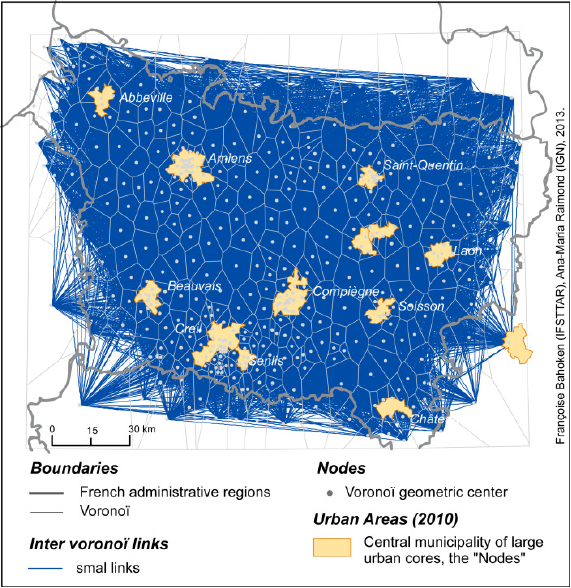
\includegraphics[width=10cm,keepaspectratio=true]{spaghetti_effect}
		\caption{\textit{Spaghetti-effect} - problem koji se mo�e javiti kod grafi�kog prikaza tokova matrice visoke prostorne i niske vremenske rezolucije. Na slici su prikazani jednodnevni tokovi.  \cite{Bahoken:2013.}}
		\label{fig:spaghetti}
	\end{center}
\end{figure}


\section{Strukturalna sli�nost \glstext{pom}}
 
Dosada spomenute mjere ne�e uhvatiti strukturalnu sli�nost matrica. Nekolicina autora isti�e va�nost strukturalne sli�nosti s referentnom matricom kao va�nu mjeru kvalitete matrice jer visoka razina strukturalne sli�nosti mo�e biti prisutna i kod matrica s manjom razinom sli�nosti prema statisti�kim mjerama. Tako�er, strukturalna sli�nost je (vizualno) vidljiva u grafi�kom obliku matrice. \textbf{Dobro odgovara ljudskoj vizualnoj percepciji sli�nosti slike}.  
 
\subsection{MSSIM} 

\gls{mssim} dolazi iz podru�ja ra�unalne obrade slike i koristi se kao mjera usporedbe digitalnih slika (\textit{eng. measure of comparison)}. U prometu ideja o kori�tenju  \gls{mssim} za mjerenje sli�nosti matrica prvi se puta spominje i demonstrira na simuliranim matricama dobivenim iz referentne matrice dodavanjem �uma. \cite{Djukic:2013.}

Informacija o strukturi slike definira se kao atributi slike koji predstavljaju strukturu objekata na sceni, i neovisni su o prosje�nom osvjetljenju i kontrastu. Jer osvjetljenje i kontrast mogu znatno varirati na sceni, moraju se u obzir uzeti samo njihove lokalne vrijednosti.

\gls{ssim} bazira se na degradaciji strukturalnih informacija na jednoj slici u usporedbi s drugom (referentnom) slikom. \gls{ssim} se ra�una za svaki kvadratni blok veli�ine %$N \times N$ (???) 
$N$ elemenata na na�in da se jezgra (da bi obuhvatila novi blok) pomi�e �eliju po �eliju dok ne pro�e preko cijele slike. \gls{mssim} je srednja vrijednost svih \gls{ssim}.


%We define the structural information in an image as those attributes that represent the structure of objects in the scene, independent of the average luminance and contrast. Since luminance and contrast can vary across a scene, we use the local luminance and contrast for our definition

\subsubsection{Osnovni}

\begin{comment}
Neka reci matrice predstavljaju polazi�ta $i, i=1,2,...I$ a stupci odredi�ta $j, j=1,2,...J$ putovanja. Da bi se odredila strukturalna sli�nost izme�u dvije matrice, neka su $d = \{d_n| n = 1,2,...,N\} $ i $\hat{d} = \{\hat{d}_n| n = 1,2,...,N\}$ dva vektora izvu�ena s iste pozicije iz referentne matrice $D=\{d_i,j\}$ i procijenjene matrice $D=\{\hat{d}_i,j\}$.

SSIM(d,\hat{d}) =[l(d,\hat{d})^\alpha][c(d,\hat{d})^\beta][s(d,\hat{d})^\gamma]\label{eq:ssim}
\cite{Djukic:2013.}
\end{comment}


%X and Y are the images to be compared (computed as matrices of pixels), and x ? fxiji ? 1; 2;:::;Ng and y ? fyiji ? 1; 2;:::;Ng are pairs of local square windows (computed as submatrices of pixels) of X and Y, respectively; x and y are located at the same spatial position in both images. SSIM is defined in terms of the average pixel values, ?x and ?y, with pixel value standard deviations (SD) ?x and ?y at patches x and y and covariance (cross-correlation) ?xy of x and y through the following indexes

Neka su $X$ i $Y$ matrice koje uspore�ujemo a  $x = \{x_n| x = 1,2,...,N\} $ i $y = \{y_n| y = 1,2,...,N\}$ parovi vrijednosti kvadratnih prozora veli�ine jezgre na istim pozicijama u  $X$ i $Y$; $SSIM$ je odre�en prosje�nim vrijednostima $\mu_x$ i $\mu_y$ sa standardnim devijacijama $\sigma_x$ i $\sigma_y$ i kovarijancom $\sigma_xy$ 


\begin{equation}
l(x,y) = (2\mu_x\mu_y +C1)/(\mu_x^2+\mu_y^2 +C1)\label{eq:l}
\end{equation}
\begin{equation}
c(x,y) = (2\sigma_x\sigma_y +C2)/(\sigma_x^2+\sigma_y^2 +C2)\label{eq:c}
\end{equation}
\begin{equation}
s(x,y) = (\sigma_xy+C3)/(\sigma_x\sigma_y +C3)\label{eq:s}
\end{equation}
%The l?x; y? index is related with luminance differences, c?x; y? with contrast differences, and r?x; y? with structure variations between x and y.

$l(x,y)$ opisuje razliku u osvjetljenju, $c(x,y)$ razliku u kontrastu, a s(x,y) razliku u strukturi izme�u $x$ i $y$. $C1$, $C2$ i $C3$ su konstante uvedene da se izbjegne "nestabilnost" kada su nazivnici bliski 0.
Op�a forma $SSIM$ definira se kao

\begin{equation}
SSIM(x,y) =[l(x,y)^\alpha][c(x,y)^\beta][s(x,y)^\gamma]\label{eq:ssim}
\end{equation}
%where ?, ?, and ? are parameters that define the relative importance of each component
gdje su $\alpha$, $\beta$ i $\gamma$ parametri relativne va�nosti svake komponente. Za $SSIM$ vrijedi slijede�e:
	\begin{subequations}
	\begin{align}
		SSIM(x,y)\leq 1  	\label{subeq:boundry} \\
		SSIM(x,y) = SSIM(y,x)		\label{subeq:simetrical}\\
		SSIM(x,y) = 1 \iff x = y \label{subeq:unique_maximum} 
	\end{align}
	\label{subeq:obje}
	\end{subequations}

\begin{equation}
MSSIM(X,Y) =  \frac{1}{M} \sum_{m=1}^{M} SSIM(x_m,y_m) \label{eq:mssim}
\end{equation}
%\cite{Renieblas:2017.}


\begin{figure}[!htpb]
	\begin{center}
		\subfloat[U odnosu na referentnu \textit{grand truth} \gls{pom}-u a), vrijednost metrike to�nosti MSE jednak je za obje matrice b) i c), dok se indeks strukturalne sli�nosti znatno razlikuje, gdje \gls{pom}-a b) ima ve�u strukturalnu sli�nost s a) nego �to ima c). Podsjetimo se da za \gls{ssim} vrijedi (\ref{subeq:obje}). Lako je na matrici c) \textit{golim okom } uo�iti naru�enost strukturalne sli�nosti. ]{\label{fig:mssim_1}
			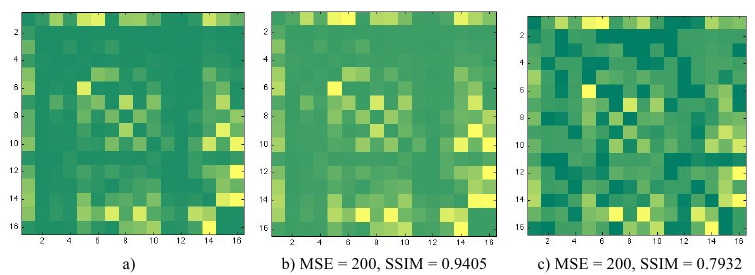
\includegraphics[width=14cm,keepaspectratio=true]{mssim_1}}\\ 
		%\hspace{10pt}
		\subfloat[U odnosu na referentnu \gls{pom}-u a), vrijednost metrike strukturalne sli�nosti iznosi 0.904 za obje matrice b) i c), dok se MSE razlikuje (ve�i MSE zna�i ve�u razliku). Obje matrice dobivene su dodavanjem Gaussianovog �uma na referentnu matricu.]
		{\label{fig:mssim_2}
			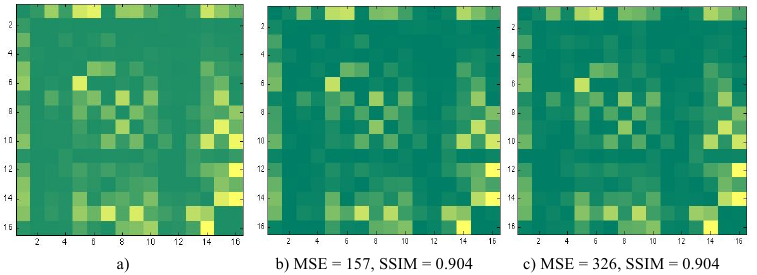
\includegraphics[width=14cm,keepaspectratio=true]{mssim_2}}
		\caption{Naru�enu strukturalnu sli�nost lak�e je uo�iti nego naru�en MSE. \gls{ssim} (i \gls{mssim})  u odnosu na referentnu POM-u mo�e biti kori�ten kao dodatna informacija (\textit{goodness of fit} mjera)  prilikom validacije POM-e \cite{Djukic:2013.}} 
		\label{fig:mssim}
	\end{center}
\end{figure}


\subsubsection{Pobolj�ani} 
Nekoliko godina nakon prvog spominjanja $MSSIM$ kao metrike usporedbe \gls{pom}-a \cite{Vuren:2015.}  se doti�e 3 problema postavljaju�i pitanja : Koliko treba biti veliki blok? Kako usporediti "guste" i "rijetke" matrice? Koja je prihvatljiva vrijednost $MSSIM$? Autori definiraju pobolj�ani model koji nazivaju $4D$-$MSSIM$ gdje u izra�un dodaju stvarne euklidske udaljenosti prostornih zona. 
    
 

% !TeX encoding = windows-1250
\chapter{Odnosni parametri kvalitete}

%Parametar se definira tako i tako

Parametar - varijabla o kojoj ovisi odre�eni logi�ki izraz, matemati�ka formula ili funkcija, a koju promatramo kao dodatnu ovisnost u izrazu koji se definira kao da je ta vrijednost �vrsta.

\section{Zajedni�ki, objektivni kriteriji usporedbe}

-Isti grad\\
-Isto doba godine\\
-Isto vremensko razdoblje
-Week day, work day

Kod generiranja matrica treba definirati ho�e li se putovanja koja se prote�u kroz vi�e perioda dodijeliti vremenskom periodu u kojem zapo�inju ili u kojem zavr�avaju. Iako ponekad nije specificirano, \cite{Bera:2011.} \cite{Filic:2016.} sva putovanja dodjeljuju intervalu u kojem je putovanje zapo�eto. 
cite{Netko:nekad} Ne zanemaruje one zapise iz kojih nije jasno vidljiv po�etak putovanja ve� takva putovanja dodjeljuje na osnovu vjerojatnosti da je zapo�elo u odre�enom periodu.

-Ima li matrica diagonalu? - kada se preslikava bs �elije na drugi oblik, 
nastaju putovanja unutar novih �elija (koje su ve�e od bs �elija) \cite{Graells-Garrido:2016.}  

\section{Komparacijski indikatori}

\subsection{Prostorna razlu�ivost (Rezolucija)}

Prema hrvatskoj enciklopediji definicija razlu�ivosti (rezolucije) glasi: mjera za razaznavanje sitnih pojedinosti na nekom prikazu (npr. televizijskoj slici). U ra�unalstvu se odnosi na fino�u rasterske slike iskazanu ukupnim brojem slikovnih elemenata (relativna razlu�ivost) ili brojem slikovnih elemenata po in�u (stvarna razlu�ivost).
(...)\\
Kod \gls{pom} ...\\
Rezolucija �e ovisiti o to�nosti polo�aja ...

Voronoi �elije tako�er je mogu�e ugnijezditi (�to se �esto radi kod usporedbe s matricama dobivenim drugim postupkom),a pritom se mo�e u matricu zabilje�iti i aproksimacija internog toka, odnosno broja putovanja unutar nove �elije (popuniti dijagonalu). Postotak eksternih putovanja koji se gubi u procesu agregacije Voronoi �elija analiziran je  za matrice iz regije Picardie u Francuskoj \cite{Bahoken:2013.}. 

Agregacijom na razinu \textit{Urban Areas} (gradova) 85\% svih putovanja postaje internim putovanjima, a na razini \textit{Urban Cores} �ak 97\% po�etno zabilje�enih putovanja je interno, te ostaje samo 3\% eksternih putovanja.

Ruralna podru�ja rje�e zahtijevaju agregiranje �elija.



Na temelju usporedbi matrica kretanja u 4 razli�ita grada, dobivenih iz \gls{cdr} i iz anketa, gdje je svaki grad u anketnim matricama imao svoju prostornu podjelu odnosno rezoluciju, Toole u svom radu \cite{Toole:2015.} (o�ekivano) zaklju�uje da sa \textbf{smanjenjem rezolucije (visokim stupnjem agregacije Voronoi �elija) stupanj korelacije s matricama iz ankete raste}. 


\begin{figure}[!htbp]
	\begin{center}
		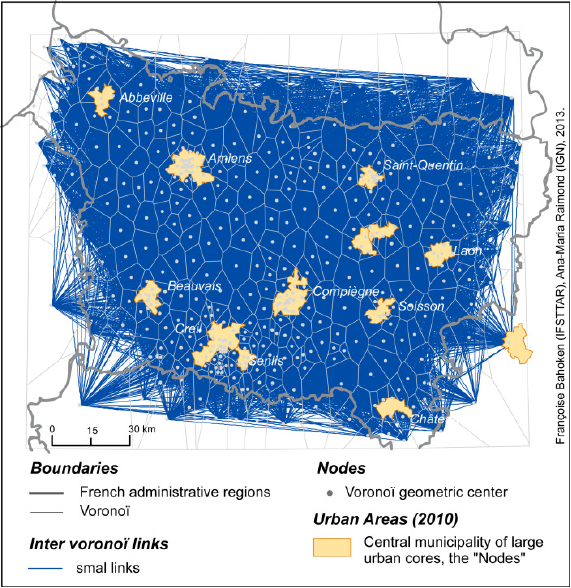
\includegraphics[width=10cm,keepaspectratio=true]{spaghetti_effect}
		\caption{\textit{Spaghetti-effect} - problem koji se mo�e javiti kod grafi�kog prikaza tokova matrice visoke prostorne rezolucije.  \cite{Bahoken:2013.}}
		\label{fig:spaghetti}
	\end{center}
\end{figure}

\subsection{Vremenska razli�ivost}

Departure/Arrival time

\subsubsection{Dani u tjednu - radni dani/petak/vikend}

\subsubsection{Sezonske razlike}


\subsection{�irina toka}

Ukupan broj odlazaka/dolazaka po vremenskom okviru za cijelu matricu.\\
-Obuhva�a pje�a�ki promet\\
- veli�ina uzorka (postotak stanovni�tva)

%\subsection{Geometrija prostorne podjele}
%(ne)uniformna podjela ...
%Interpolacija - ima li smisla 2 razli�ite podjele?!

\subsection{Definicija putovanja}

prosje�an broj putovanja po stanovniku/ispitaniku

\subsubsection{Infrastruktura}
Obuhva�a pje�a�ki promet
%\subsubsection{Sredstvo kretanja}

\subsection{Gusto�a informacija - kontekst}


\section{Me�uovisnost parametara}
Ukoliko je rezlucija mala (velike �elije) nema potrebe za preciznim definiranjem kraja putovanja

\begin{comment}
2 modela
PoV (Predicted vs Observed)

Robusnost matrice ->una�anje �uma

\cite{Zhao:2017.} kad spominje TAD
\end{comment}

 % itd.
%% !TeX encoding = windows-1250
\chapter{Metodologija usporedbe}

\section{Podaci}

\section{Rezultati}

 % itd.
% !TeX encoding = windows-1250
\chapter{Zaklju�ak}
% Zaklju�ak � u kojemu se sa�imaju rezultati rada. U pravilu Zaklju�ak ne bi trebao biti du�i od dvije stranice. 

Establishing access policies for spatial information is a pressing societal need
requiring a better understanding of all values involved. It is complicated by the fact that information about indoor and geographic spaces gets collected and shared by almost everybody. This phenomenon of crowd-sourced or Volunteered Geographic Information (VGI, (Goodchild 2007)) is profoundly altering the values related to spatial information, from economic as well as institutional, ethical, and legal perspectives. 
http://www.economist.com/node/1788311

% !TeX encoding = ASCII
%I) rucno upisati svaku referencu redoslijedom kojim se prvi puta pozivaju u tekstu
%\begin{thebibliography}{99}
%
%\bibitem{html} .....opis reference .........
%
%\bibitem{php} .......opis reference ........
%
%\bibitem{ajax}  .........opis reference..........
%
%\end{thebibliography}



%II) bolji nacin: pomocu programa JabRef opisati svoje reference i pohraniti u datoteku ``Literatura.bib''. U tekstu samo pozivati zeljene reference, a lista se sama formira.

\bibliographystyle{tex_aux/IEEEtranHR}  % ``unsrt'', ``IEEEtran'', ``ieeetr''
% argument is your BibTeX string definitions and bibliography database(s)

\bibliography{Literatura}
  % ovo je ime Bibtex datoteke koju korisnik kreira


%:::::::::: ukljucenje popisa kratica u tekst ::::::::
% Blok linija koda ispod ovoga generira ukljucenje popisa kratica u tekstu. Za uporabu, vidjeti Upute.
% Nije obavezno. Ako se ne zeli koristiti, onda ovaj blok staviti u komentar pomocu znaka %
\printglossary[type=\acronymtype]
\pagestyle{plain}
\begin{glossary}{Longest string}
	% !TeX encoding = windows-1250
%%%%%%%%%%%%%%%%%%%%%%%%%%%%%%%%%%%%%%%%%%%%%%%%%%%%%%%%%%%%%%%%%%%%%%%%%%%%%%%%%%%%%%%%%%%%%%%%%
%% ovo je jednostavniji (ali neautomatski) primjer definiranja liste akronima, a student neka to zamijeni svojim kraticama i doda sve koje zeli
%% ako se ne zeli deklarirati popis kratica, onda ga staviti pod komentar u glavnoj datoteci
%
%   \item[{\bf HTML}]	Hypertext Markup Language
%   \item[{\bf AJAX}]	Asynchronous JavaScript and XML

%%%%%%%%%%%%%%%%%%%%%%%%%%%%%%%%%%%%%%%%%%%%%%%%%%%%%%%%%%%%%%%%%%%%%%%%%%%%%%%%%%%%%%%%%%

%%%%%%%%%%%%%%%%%%%%%%%%%%%%%%%%%%%%%%%%%%%%%%%%%%%%%%%%%%%%%%%%%%%%%%%%%%%%%%%%%%%%%%%%%%
% Sofisticiraniji nacin definiranja i uporabe kratica je preko sljede�e sintakse

 \addcontentsline{toc}{chapter}{Pojmovnik}
% primjeri definicije kratica
% ove pojmove zamijenite nekim svojima i po tom predlosku nadogradite listu po potrebi
\newacronym{pom}{POM}{Polazi�no-odredi�na matrica (Izvori�no-odredi�na matrica) }
\newacronym{taz}{TAZ}{Traffic Analisys Zone}
\newacronym{iom}{IOM}{Izvori�no-odredi�na matrica}
\newacronym{odm}{ODM}{Origin-Destination Martix} 
\newacronym{cdr}{CDR}{Call Data Records ili Charging Data Records} 
\newacronym{gsm}{GSM}{Global System for Mobile (Communications)}
\newacronym{rsi}{RSI}{Road Side Interview}
\newacronym{pois}{POIs}{To�ke interesa (engl. Points of Interest)}
\newacronym{hw}{HW}{Home-Work}
\newacronym{wh}{WH}{Work-Home}
\newacronym{ebm}{EBM}{Work-Home}
\newacronym{ssim}{SSIM}{Indeks strukturalne sli�nosti (engl.  Structural Similarity Index)}
\newacronym{mssim}{MSSIM}{Vi�e-razinski indeks strukturalne sli�nosti (engl. Mean Structural Similarity index)}
\newacronym{anpr}{ANPR}{Automatic Number Plate Recognition}
\newacronym{fcd}{FCD}{Floating Car Data}
\newacronym{fpd}{FPD}{Floating Phone Data (Floating Cellular Data)}
\newacronym{gnss}{GNSS}{Global Navigation Satellite System}
\newacronym{gps}{GPS}{Global Positioning System}
\newacronym{gis}{GIS}{Geoprostorni informacijski sustav}
\newacronym{osm}{OSM}{OpenStreetMap}
\newacronym{d4d}{D4D}{Data for Development}
\newacronym{its}{ITS}{Inteligentni transportni sustav (engl. \textit{Intelligent Transportation System})}
\newacronym{gdpr}{GDPR}{General Data Protection Regulation}
\newacronym{sms}{SMS}{Short Messaging System}
%::::::::: UPORABA KRATICA U TEKSTU :::::::::::::::::
% u tekstu jednostavno na mjestu gdje �elite koristiti odre�enu kraticu, upotrijebite naredbu 
%  \gls{id_kratice}, kao npr. \gls{nfc}
% i u tekstu �e vam automatski biti uba�ena kratica kako je definirana u drugoj zagradi u gornjim definicijama, a ako je u uporabi prvi puta, tada �e prvo biti naveden puni naziv, kako je definiran u tre�oj zagradi, a potom kratica. Za sve ostale slu�ajeve uporabe, bit �e navedena samo kratica.

%:::::::::::::::::::::::::::::::::::::::::::::::::::::
%  podsjetnik nekoliko mogu�ih oblika sintakse
% op�a uporaba: \gls{nfc} % mo�e i za rje�nik i za kratice. Prvi poziv daje dugi i kratki naziv (redoslijedom koji je specificiran u preambuli pomocu \setacronymstyle, a od drugi puta nadalje samo kraticu.
% ako �elite nametnuti ba� neki oblik kori�tenja kratice, imate sljede�e naredbe
%\acrshort{nfc} \\  % samo akronim
%\acrfull{nfc} \\   % akronim i puni naziv
%\acrlong{nfc} \\   % samo puni naziv

%::::::::::::::::::::::::::::::::::::::::::::::::::::
% Kako se generira Pojmovnik u tekstu:
%1. pokrenite LaTeX kompilaciju 1x
%2. u Command Promptu odite radnu mapu gdje su vam datoteke diplomskog rada i utipkajte
%	makeindex -s myDoc.ist -o myDoc.gls   myDoc.glo
%	
%	gdje myDoc zamijenite imenom svoje glavne .tex datoteke (JMBAG_Ime_Prezime.tex)
%3. pokrenite LaTeX kompilaciju jos jednom

%::::::::::::::::::::::::::::::::::::::::::::::::::::
\end{glossary}


%:::::::::::: blok za definiranje Sazetka/Abstracta rada 
\begin{abstract}
	% !TeX encoding = windows-1250
\vspace{5pt}

%:::::::::::::::::::::::::::::::::::::::::::::::::::::
%:::::::::::: HRVATSKI :::::::::::::::::::::::::::::::
\noindent

\glsfirst{pom} %Izvori�no-Odredi�na ili 
%\textit{eng. \gls{odm}} ili \textit{Trip Table} 
(POM) je alat koji omogu�uje opis i sustavnu statisti�ku procjenu migracija stanovni�tva na nekom podru�ju u zadanom prostorno-vremenskom okviru. \gls{pom}-a slu�i za opis grupne mobilnosti i mjerenje socio-ekonomske aktivnosti u nekoj regiji, a naj�e��e se koristi u prometnoj znanosti za analizu i strate�ko planiranje prometnog optere�enja i prometne infrastrukture. Postoje brojni tradicionalni pristupi procjeni i vrednovanju \gls{pom}-a, a dolaskom pasivno prikupljanih suvremenih izvora podataka o kretanju (zapisi usluga baziranih na lokaciji) omogu�en je razvoj suvremenih pristupa i pro�irenje podru�ja primjene. 
Postupci procjene koji uklju�uju kontekstualizaciju dnevnih migracija daju uvid u motive odnosno svrhu kretanja stanovni�tva. Postoje�e metode vrednovanja \gls{pom}-a definiraju vrijednost nove \gls{pom} usporedbom i razmatranjem sli�nosti s postoje�om za isto podru�je.  Postoji potreba da se definira i kvantizira kvaliteta \gls{pom}-e kroz objektivne parametre. Ovaj rad predstavlja alternativni pristup vrednovanju \gls{pom}-a, definira objektivne parametre kvalitete, uvjete usporedbe i postupak odlu�ivanja o kvaliteti \gls{pom}. Definirana metodologija obuhva�a kontekstualizaciju kao dio kvalitete \gls{pom}. Metodologija je demonstrirana na usporedbi dvije \gls{pom} dobivene iz razli�itih izvora razli�itim postupcima procjene.
%i tako pro�iruje podru�je primjene \gls{pom} i analize kretanja stanovni�tva op�enito. 
%Kontekstualizacija omogu�uje izdvajanje visoko repetitivnih, a time i predvidivih kretanja, od nepredvidivih kretanja

%Ovo je tekst u kojem se opi�e sa�etak va�ega rada. Tekst treba imati duh rekapitulacije �to je prikazano u radu, nakon �ega slijedi 3-5 klju�nih rije�i (zamijenite dolje postavljene op�enite predlo�ke rije�i nekim suvislim vlastitim klju�nim rije�ima).
%:::::::::::::::::::::::::::::::::::::::::::::::::::::

\vspace{5pt}
%
\noindent \textbf{\textit{Klju�ne rije�i} --- Polazi�no-odredi�na matrica (Izvori�no-odredi�na matrica), kontekstualizacija, parametri kvalitete, usporedba, vrednovanje} 

%:::::::::::: KRAJ HRVATSKOG DIJELA :::::::::::::::::::


%::::::::::::::::::::::::::::::::::::::::::::::::::::::
%:::::::::::: ENGLESKI ::::::::::::::::::::::::::::::::

%\vspace{-10pt}
\section*{Abstract}
\vspace{-10pt}
%This is a text where a brief summary of your work is outlined. The text should have a sense of recap of what was presented in the thesis, followed by 3-5 keywords (replace the general keyword templates below with some meaningful keywords of your own) .
%:::::::::::::::::::::::::::::::::::::::::::::::::::::::
Origin-Destination Matrix (ODM) is a tool that enables description and systematic statistical estimation of human migrations in an area and within a give space-time frame. ODM is used to describe group mobility and measure socio-economic activity in a region, and is most commonly used in transport science for the analysis and strategic planning of transport load and transport infrastructure. There are a number of traditional approaches to ODM estimation and evaluation.  The rise of passively collected location data (from location based services) has enabeld development of new, modern approaches and broadens the field of use. Approaches that involve contextualisation of daily migrations provide insight into the motives and te purpose of urban movements. The existing ODM valuation methods define the value of a new ODM by comparing it to an existing ODM and conidering the simmilarity. There is a need to define and quantify the quality of ODM through objective parameters. This thesis presents an alternative approach to ODM evaluation, defines objective quality parameters, comparison conditions and decision process. Defined methodology captures contextualization as part of ODM quality. The methodololgy is demonstrated with comparing two ODMs obtained from different sources and with different estimation procedures.

\vspace{5pt}
%
\noindent \textbf{\textit{Keywords} ---Origin-Destination Matrix (Trip Table), contextualization, quality parameters, comparation, evaluation}

%::::::::::::::::::::::::::::::::::::::::::::::::::::::
%:::::::::::: KRAJ ENGLESKOG DIJELA :::::::::::::::::::

	  % sazetak rada i kljucne rijeci na HR i EN
\end{abstract}


%:::::::::::: PRILOZI (neobavezno) ::::::::::::::::::::
% ispod \appendix zaglavlja pomocu \include dodati poglavlja s prilozima
% ukoliko nemate priloga, ovaj blok linija staviti u komentar
\appendix
% !TeX encoding = windows-1250
\chapter{Metrike za vrednovanje polazi�no-odredi�ne matrice}
\label{dodatak_metrics}

\subsection{Metrike za procjenu sli�nosti polazi�no-odredi�ne matrice s referentnom}

Za procjenu kvalitete \gls{pom}-a dobivenih isklju�ivo anketranjem u radu \cite{Cools:2010.} kori�tena je mjera srednja apsolutna postotna pogre�ka (engl. Mean Absolute Percentage Error, MAPE), te je prikazano da se zadovoljavaju�a razina kvalitete takvih \gls{pom}-a posti�e ako uzorak obuhva�a 50\% populacije. Autor Cools isti�e va�nost kori�tenja drugih izvora uz ankete za izradu \gls{pom}-a.

U radu \cite{Bera:2011.} navedene su statisti�ke mjere relativna pogre�ka (engl. Relative Error, RE), devijacija ukupne potra�nje (engl. Total Demand Deviation, TDD), srednja apsolutna pogre�ka (engl. Mean Absolute Error, MAE), korijen iz srednje kvadratne pogre�ke (engl. Root Mean Square Error, RMSE) te najve�a mogu�a relativna pogre�ka (engl. Maximum Possible Relative Error, MPRE) i razina prometne potra�nje (engl. Travel Demand Scale, TDS) koji procjenjuju kvalitetu neovisno o referentnoj matrici (no MPRE ne dopu�ta pogre�ke u prebrojavanju prometa, dok TDS ovisi o topologiji mre�e i odabiru ruta) \cite{Djukic:2013.}.

U \cite{Frias-Martinez:2012.} kori�ten je \textit{Pearsonov koeficijent korelacije} -  $r$ da bi se utvrdila \textbf{sli�nost svakog retka \gls{pom}-e} dobivene iz CDR \textbf{s retkom referentne} (ukupni izlazni tok iz svake polazi�ne �elije). Isti postupak kori�ten je za kontekstualizirane \gls{hw} i \gls{wh} \gls{pom}-e  dobivene iz \gls{cdr} u usporedbi s referentnim \gls{pom}-ma dobivenim anketiranjem. %**

U svome radu \cite{Travassoli:2016.} navodi se nekoliko mjera - {$R^{2}$, Geoffrey E. Havers statistika (GEH),  korijen iz postotak srednje kvadratne pogre�ke (engl. Root Mean Squared Error percentage, \%RMSE), uvodi novu mjeru  Eigenvalue-Based Measure (EBM) (temeljenu na svojstvenim vrijednostima matrica) i procjenjuje pouzdanost \gls{pom}-e dobivene iz sustava automatskog prikupljanja podataka u javnom prijevozu (autobus, vlak i trajekt). Spominje i Wasserstein metriku, mjeru koja ne uspore�uje samo vrijednosti parova istih �elija (\textit{elementwise}). 
	
Spearmanov koeficijent korelacije ranga kori�ten je u \cite{Graells-Garrido:2016.} za procjenu sli�nosti \gls{pom}-a dobivenih iz \gls{cdr} sa tada aktualnim \gls{pom}-ma dobivenim anketiranjem.
	
	%(...)
	%Dynamic Travel Demand \cite{Gundlegard:2016.}
	
	\begin{comment}
	
	mozda po jednu recenicu za svako
	\subsubsection{$R^{2}$ }
	The R-squared (R2), as one of the most commonly and widely used (Washington et al., 2011), is a statistical measure of how close the data are to the fitted regression line, and itused for comparing between origin-destination pairs of two ODMs. R2 values rang from 0 to 1, with higher values indicating less difference between ODMs. 
	Along with considering higher value of R2 as a higher level of similarity, the regression line should be close to a 45-degree line through the origin. In this condition, the coefficient of the line should be closer to one and the intercept should be closer to zero. The lower and greater coefficient values indicate the tendency of the pattern to overestimate or underestimate values in the reference OD matrix.\cite{Travassoli:2016.}
	
	\subsubsection{GEH}
	Geoffrey E. Havers (GEH) statistic
	The GEH statistic is used to evaluate the level of closeness between origin-destination pairs of two ODMs. The GEH is applied to every pair in the two ODMs, with a GEH of less than 5 indicating a good fit (Hollander and Liu 2008). Then, the percentage of OD pairs that have a GEH equal to or less than 5 is calculated to indicate the level of closeness between two ODMs.
	\cite{Travassoli:2016.}   
	
	\subsection{RMSE i \%RMSE} 
	The root mean squared error (RMSE) and accordingly the percent root mean squared error(%RMSE) are used to evaluate the closeness of the ODMs. The %RMSE is where the variability of the demand is most evident: if two demand ODMs were identical, the %RMSE would be equal to zero.
	\subsubsection{ MSE, SEM, EBM (SAE)} 
	(How close the models are to the reality)
	
	\subsubsection{Pearson korelacija redova}
	
	\subsubsection{Sperman rank korelacija}
	
	\subsubsection{Wasserstein Metric} (?)
	
	\end{comment}
  % dati neko suvislo ime umjesto ovoga
%% !TeX encoding = windows-1250
\chapter{Prilagodba prostorne podjele}
\label{dodatak_ppp}

Ako je to�nost matrice definirana isklju�ivo kao sli�nost svakog njenog elementa s ekvivalentnim u elementom u \textit{grand truth} matrici nu�no je osigurati da prostorna podjela matrice odgovara prostornoj podjeli referentne ili je potrebno obje matrice svesti na zajedni�ku prostornu podjelu. 

\section{Agregacija baznih stanica}
Pregledom literature utvr�eno je da se koriste \textit{k-sredina} i \textit{mean-shift} algoritam za grupiranje baznih stanica u broj grupa jednak broju \gls{taz} na podru�ju o interesa \cite{Goulding:2016.} \cite{Alhazzani:2016.} \cite{Mellegard:2011.} ili pak jedinicama samouprave (eng. \textit{municipalities}) kako bi  \gls{pom}-e u kona�nici bile usporedive s postoje�ima, dobivenim iz anketa \cite{Coscia:2015.} \cite{Frias-Martinez:2012.}. Nije utvr�ivano kolika se gre�ka uvodi ovim postupcima. Primjer gusto�e tornjeva baznih stanica na podru�jima anketnih jedinica prikazan je na slici \ref{fig:density}
%\cite{Mellegard:2011.} ne definira unaprijed broj grupa ve� za grupaciju koristi \textit{mean-shift} algoritam koji sam odre�uje broj grupa na podru�ju �vedske, potom koriste�i \gls{osm} grupe ve�e uz imena gradova i mjesta. 
%U istra�ivanju \cite{Coscia:2015.} bazne stanice na podru�ju Kolumbije grupiraju po jedinicama samouprave (eng. \textit{municipalities}). Isti postupak je kori�ten i u istra�ivanju na podru�ju Madrida, kako bi  \gls{pom}-e u kona�nici bile usporedive s onima dobivenim iz anketa \cite{Frias-Martinez:2012.}.

\begin{figure}[!htbp]
	
	\begin{center}
		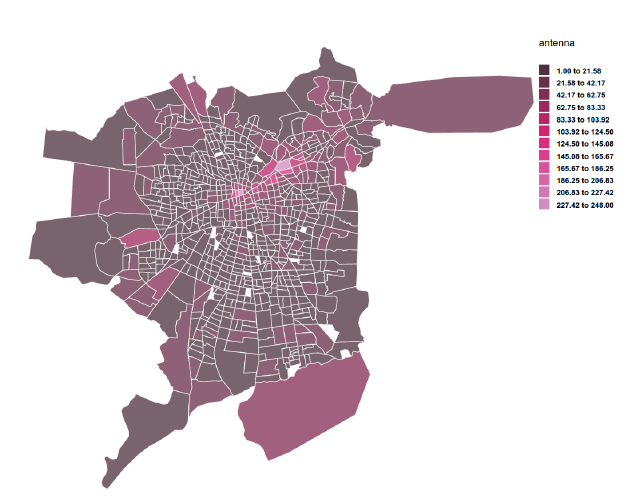
\includegraphics[width=15cm,keepaspectratio=true]{Santiago_antenna_density}
		\caption{Prostorna podjela na anketne jedinice u gradu Santiagu. Gusto�a tornjeva baznih stanica po anketnim jedinicama. Gusto�a varira od 1 do 250 tornjeva po anketnoj jedinici.
			\cite{Graells-Garrido:2016.}}
		\label{fig:density}
	\end{center}
\end{figure}


\section{Interpolacija}
\label{interpol}
Postupak konverzije \gls{pom}-a iz prostorne podjele na Voronoi �elije u drugu prostornu podjelu, npr. uniformnu kvadratnu mre�u (�elije $1 km^2$), opisan u priru�niku \cite{Goulding:2016.}. U postupku odre�ivanja postotka ukupnog toka Voronoi �elije koji �e se dodijeliti novoj kvadratnoj �eliji predla�e se uzeti u obzir: povr�inu preklapanja tih �elija, broj zgrada ili ukupnu povr�inu zgrada (uklju�uju�i katove) na podru�ju preklapanja tih �elija. 
Na slici \ref{fig:interpolation} je prikazan tre�i oblik interpolacije gdje su kori�teni podaci o ukupnoj kvadratnoj povr�ini zgrada. 

\begin{figure}[!htbp]
	\begin{center}
		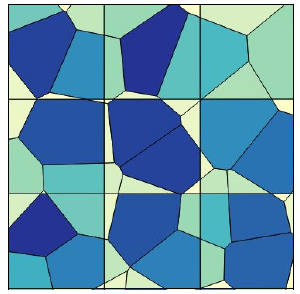
\includegraphics[width=6.5cm,keepaspectratio=true]{interpolation}
		\caption{Primjer mozaika \textit{krhotina} za interpolaciju izme�u Voronoi �elija i kvadratne mre�e. Nijansa odra�ava postotak povr�ine zgrada u \textit{krhotini} u odnosu na cijelu Voronoi �eliju kojoj pripada. Rezultat se dobiva na osnovu tih \textit{te�inskih faktora} polazi�ne i odredi�ne \textit{krhotine} te pripadaju�ih ("roditeljskih") Vornoi �elija. Sumom svih rezultata krhotina jedne kvadratne �elije izra�una se kona�ni tok. \cite{Goulding:2016.}}
		\label{fig:interpolation}
	\end{center}
\end{figure}

\section{Posljedice agregacije prostornih �elija}

Voronoi �elije tako�er je mogu�e ugnijezditi (�to se �esto radi kod usporedbe s \gls{pom}-ma dobivenim drugim postupkom), a pritom se mo�e u matricu bilje�iti i aproksimacija internog toka, odnosno broja putovanja unutar nove �elije (dijagonala matrice). Takva putovanja nazivaju se internim putovanjima. Studija \cite{Toole:2015.} je pokazala da sa \textbf{smanjenjem rezolucije (visokim stupnjem agregacije Voronoi �elija) stupanj korelacije s \gls{pom}-ma iz ankete (za isti grad) raste} (\gls{pom}-e dobivene iz \gls{cdr} i iz anketa u 4 razli�ita grada). 
Postotak eksternih putovanja koji se gubi u procesu agregacije Voronoi �elija analiziran je u studijama \cite{Graells-Garrido:2016.} (Vidi sliku \ref{fig:diagonal}) i \cite{Bahoken:2013.} za \gls{pom}-e iz regije Picardie u Francuskoj.
\textbf{Agregacijom Voronoi �elija na razinu \textit{Urban Areas} (podru�ja oko gradova) 85\% svih putovanja postaje internim putovanjima, a na razini \textit{Urban Cores} (podru�ja oko ve�ih gradova) �ak 97\% po�etno zabilje�enih putovanja je interno, te ostaje samo 3\% eksternih putovanja} \cite{Bahoken:2013.}.

\begin{figure}[!htpb]
	\begin{center}
		\subfloat[Izvor podataka anketa ]{\label{fig:survey}
			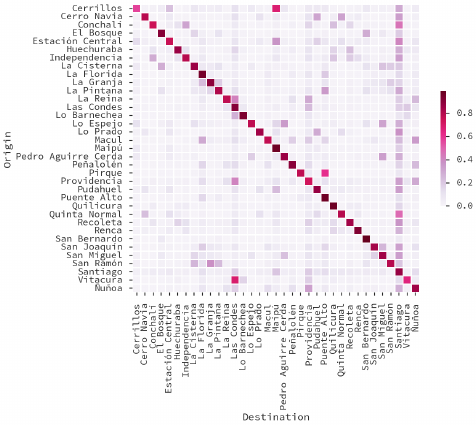
\includegraphics[height=9cm,keepaspectratio=true]{survey}}\\ 
		%\hspace{10pt}
		\subfloat[Izvor podataka \gls{cdr}]
		{\label{fig:cdr}
			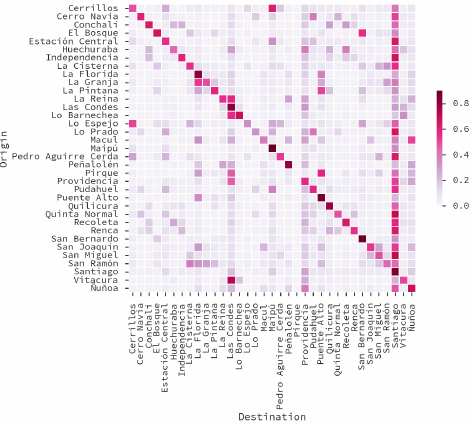
\includegraphics[height=9cm,keepaspectratio=true]{cdr}}
		\caption{Distribucija \acrshort{cdr} putovanja na podru�ju Santiaga, �ile. \gls{pom} je normalizirana prema redovima (polazi�tima) (*) \cite{Graells-Garrido:2016.}}
		\label{fig:diagonal}
	\end{center}
\end{figure}
%Ruralna podru�ja rje�e zahtijevaju agregiranje �elija.


\chapter{OpenStreetMap}
\label{dodatak_osm}
\gls{osm} je svjetski ra�iren projekt koji kreira i pru�a slobodne zemljopisne podatke (zemljovide gradova i naselja) temeljen na volonterskom doprinosu zajednice. Projekt pru�a detaljne i a�urne digitalne zemljovide kompatibilne s \gls{gis} aplikacijama. 
Zapo�et je prije 15 godina, u Ujedinjenom Kraljevstvu, kao odgovor na tehni�ka ili pravna ograni�enja postoje�ih "slobodnih" baza prostornih podataka kao �to je GoogleMaps. Zajedni�ki doprinos i me�usobna kontrola unosa odr�avaju kartu na visokoj razini kvalitete i to�nosti.

Struktura osnovnih elemenata na toj rasterskoj karti je hijerarhijska. Element u hijerarhiji mo�e biti: �vor (engl. \textit{node}), put (engl. \textit{way}) ili relacija (engl. \textit{relation}). Uz hijerarhijske postoji i opisni element koji se naziva oznakom (engl. \textit{tag}), a njegova funkcija je opisati zna�ajke hijerarhijskog elementa uz koji je vezan. 

�vor je jedinstvena to�ka u prostoru (sa identifikacijskom oznakom, zemljopisnom �irinom i du�inom) koja naj�e��e predstavlja fizi�ki objekt (zgrada, dio ceste...) te sadr�i jedan ili vi�e \textit{klju�=vrijednost} oznaka (engl. \textit{key=value tag}) koji definiraju razne zna�ajke objekta.

Put je ure�ena lista 2 do 2,000 �vorova, koja tako�er mo�e biti opisana \textit{klju�=vrijednost} oznakama. 

Relacija je ure�ena lista �vorova, puteva i/ili relacija. Definira logi�ku ili geografsku povezanost �lanova.
 
Primjeri oznaka vezanih za �vorove:  \textit{office=company}, \textit{building=residential}, \textit{building=hotel}, \textit{building=church}, \textit{leisure=sports\_centre} , \textit{amenity=school}. Primjer �iga vezanog uz put \textit{highway=residential}.

\gls{osm} doprinosi istra�ivanjima u podru�ju analize kretanja stanovni�tva i kao izvor prometne infrastrukture i pripadaju�ih meta podataka (kolnik, mostovi, ograni�enja brzine i dr.)\cite{Toole:2015.} i kao izvor podataka o podnoj povr�ini objekata (engl. floor area) \cite{Goulding:2016.}. 
%Raspodjela toka po prometnoj infrastrukturi nadilazi podru�je ovog rada no jest dio problematike modeliranja prometa.  
\chapter{Procjena Polazi�no-Odredi�ne Matrice B}
\label{dodatak_taxi}
Podatci u formatu \ref{fig:TaxiData} su grupirani prema Identifikacijskom broju i sortirani prema vremenskom �igu (Time). Po�etak putovanja definiran je kao prelazak Statusa (engl. Occupancy Status) iz $0$ u $1$, a kraj kao prelazak iz 1 u 0. Prostorna podjela POM je na Voronoi �elije oko tornjeva baznih stanica jer podatci o \gls{taz} nisu javno dostupni. Generirano je 8 \gls{pom}, a sva putovanja su dodjeljivana periodu u kojem po�inju.

\begin{figure}[!htbp]
	\begin{center}
		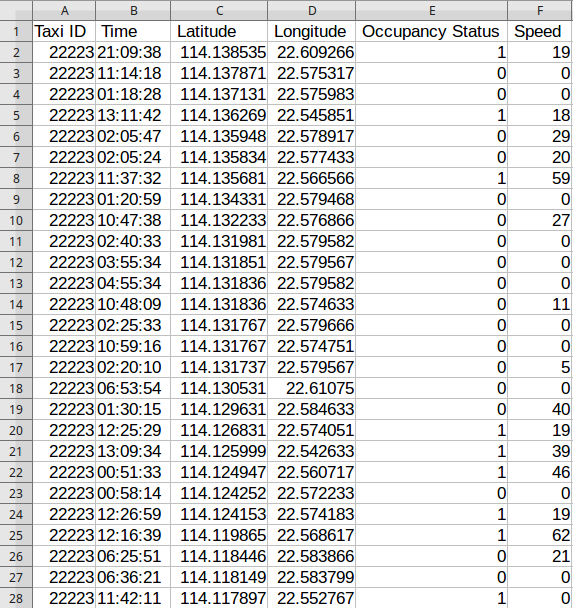
\includegraphics[width=10cm,keepaspectratio=true]{TaxiData}
		\caption{Format podataka iz kojih je procijenjena POM B}
		\label{fig:TaxiData}
	\end{center}
\end{figure}


  % itd.


\end{document}
